
\section{Supplementary Material}
    For the complete set of illustrations and measurements, please access Sciebo \cite{sciebo_data}.

\subsection{Measurements on PMMA}

% 2mm PMMA
    \begin{figure}[H]
        \centering
        \makebox[\textwidth]{
        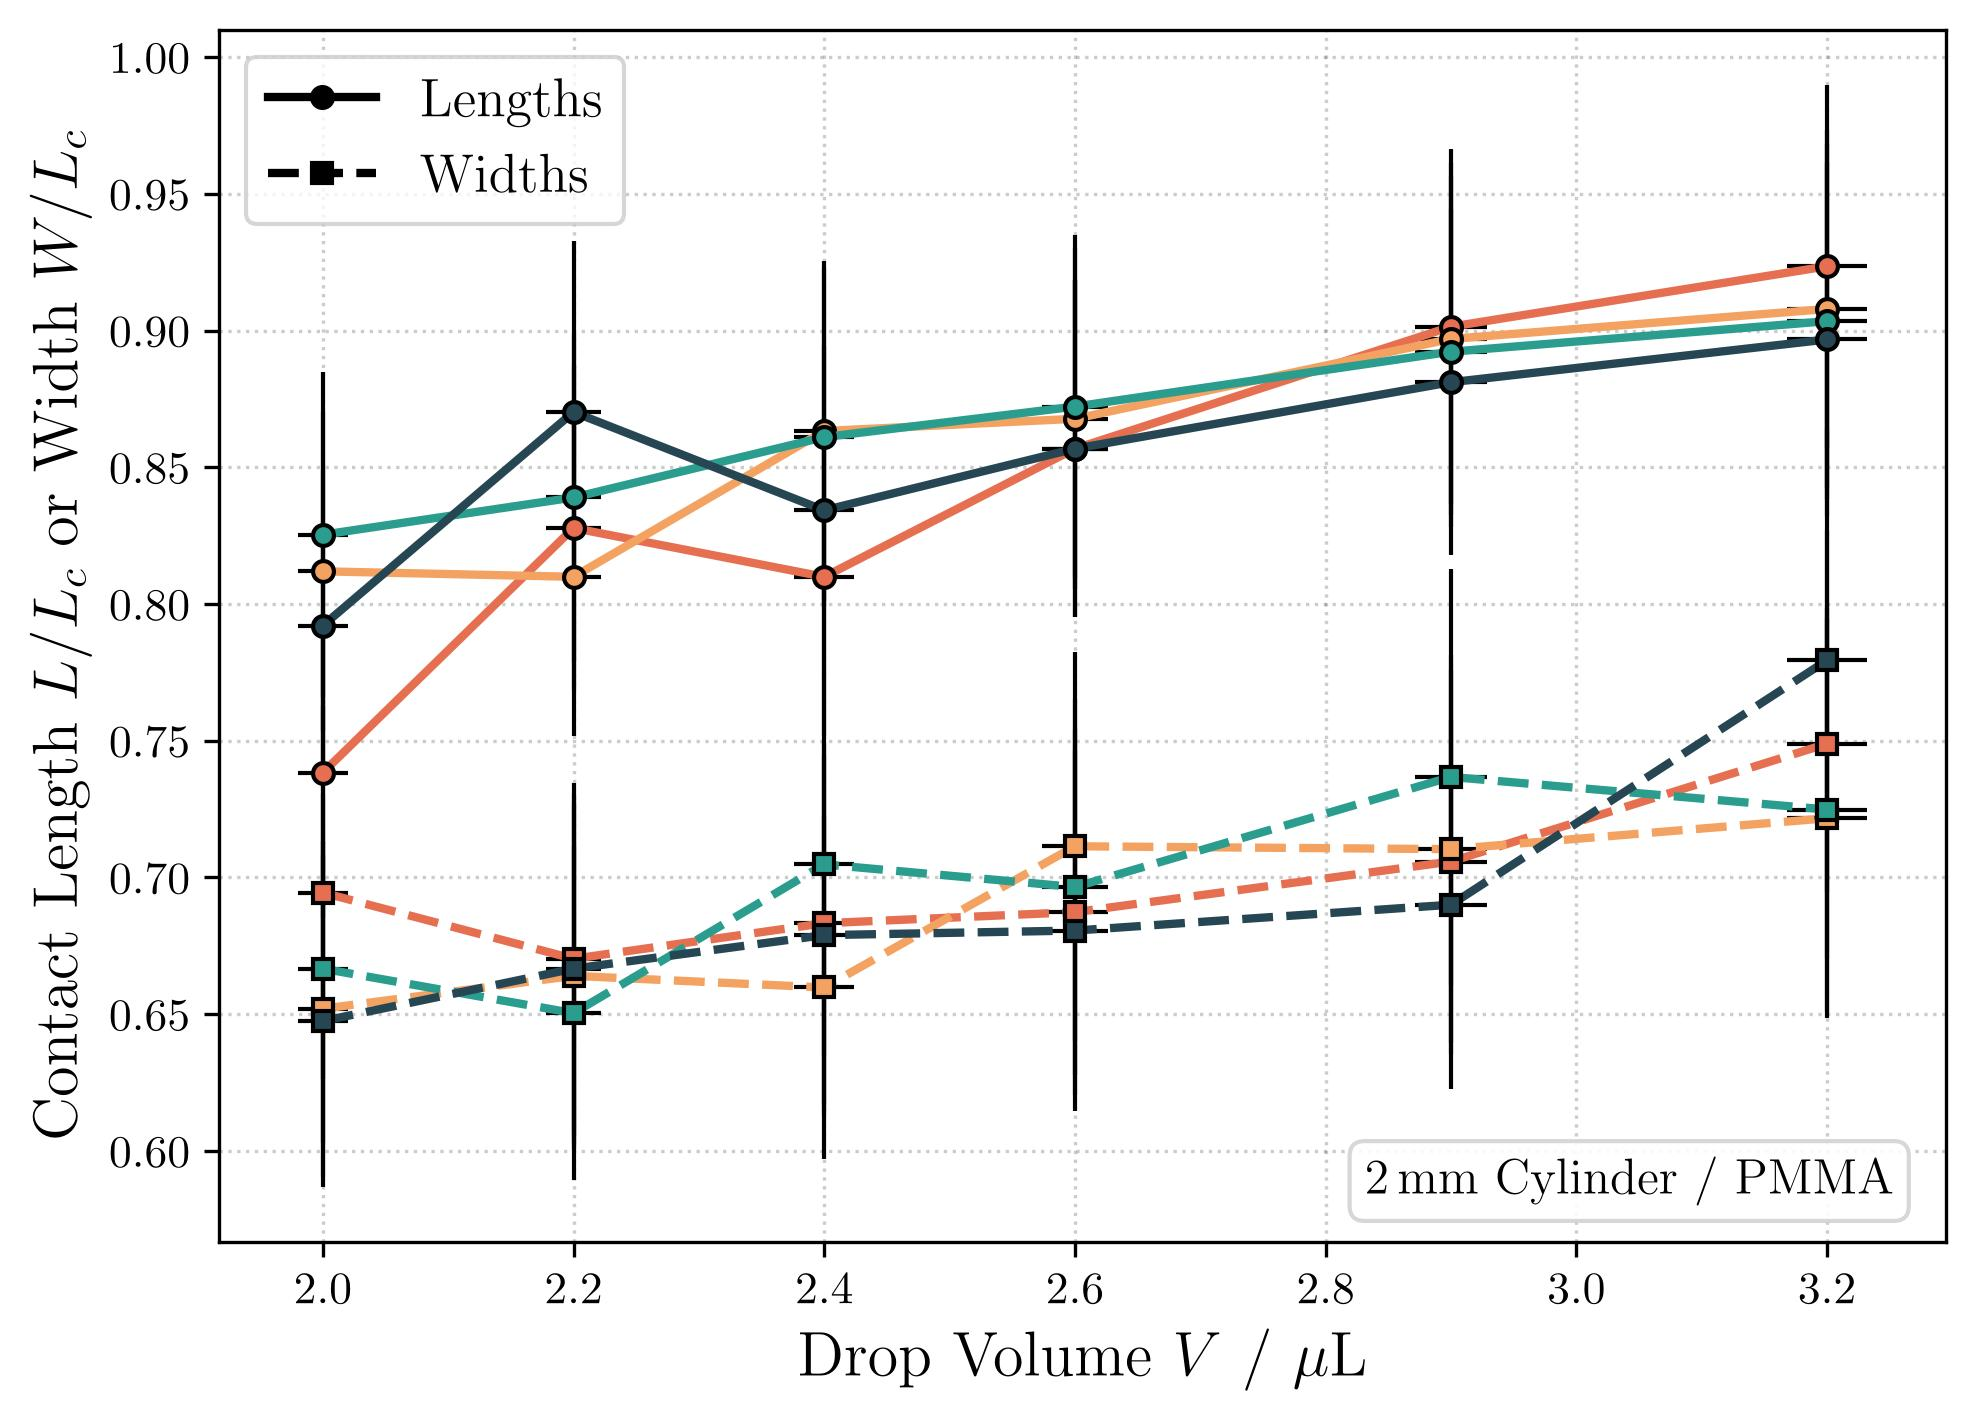
\includegraphics[width=0.55\linewidth]{../Plots/w06_02mm_PMMA_L+W.jpg}
        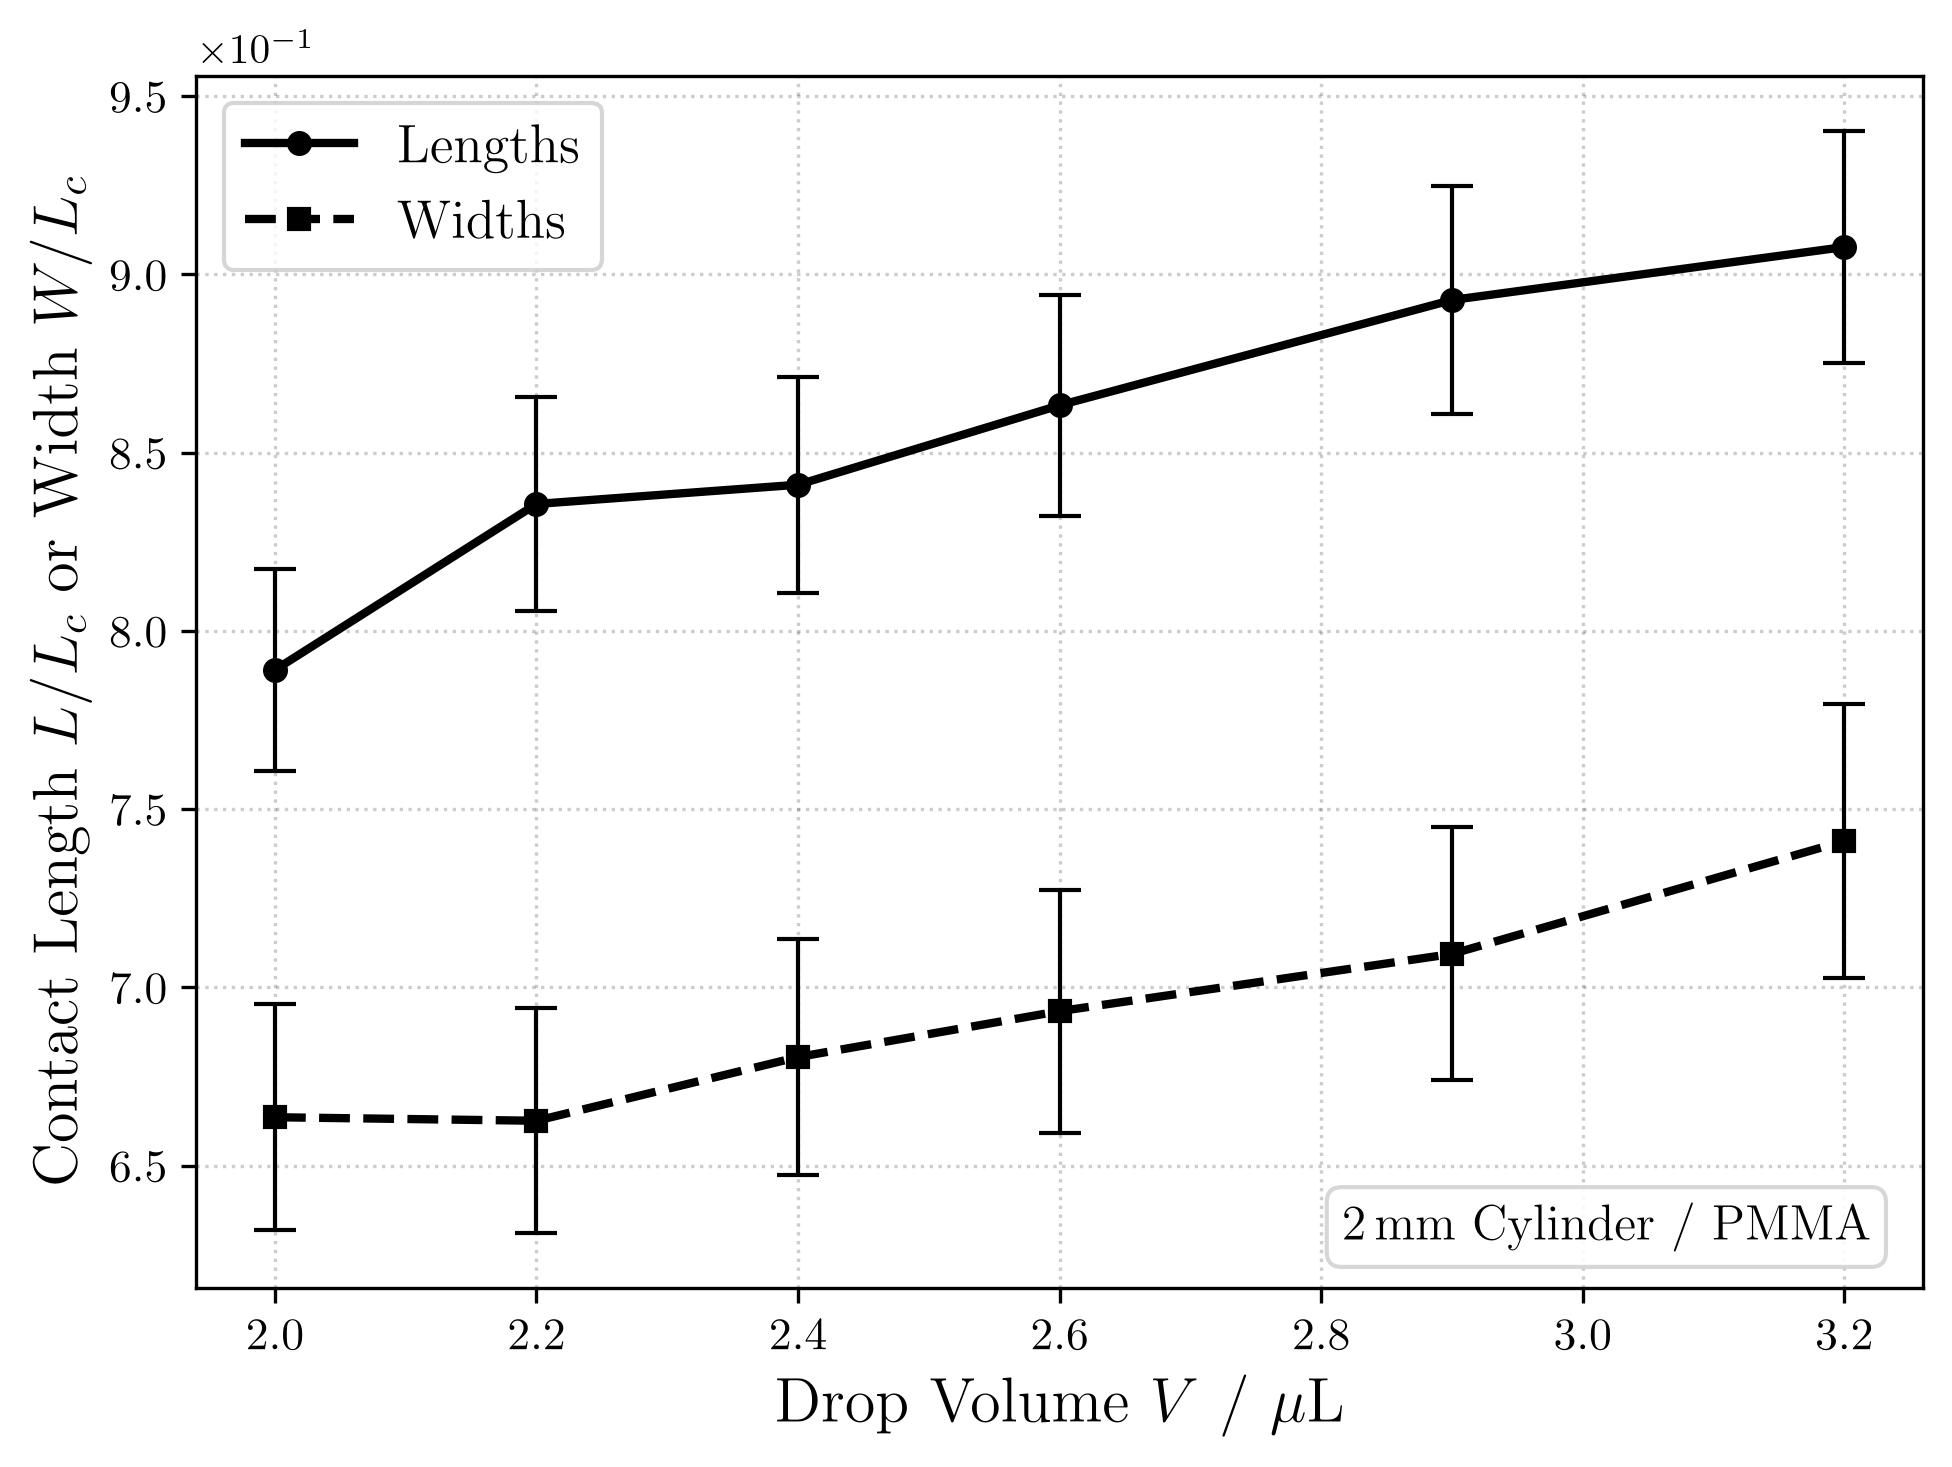
\includegraphics[width=0.55\linewidth]{../Plots/w06_02mm_PMMA_L+W_avg.jpg}
        }
        \caption{Measurements of contact length $L$ and width $W$ on the \SI{2}{\milli\meter} PMMA cylinder in raw (left) and averaged (right). The contact length $L$ along the cylinder axis always exceeds the width $W$, however, the region of interest for $V < \SI{2}{\micro\liter}$ could not be measured in practice.}
        \label{fig:app:2mm_data_PMMA}
    \end{figure}

    \begin{figure}[H]
        \centering
        \makebox[\textwidth]{
        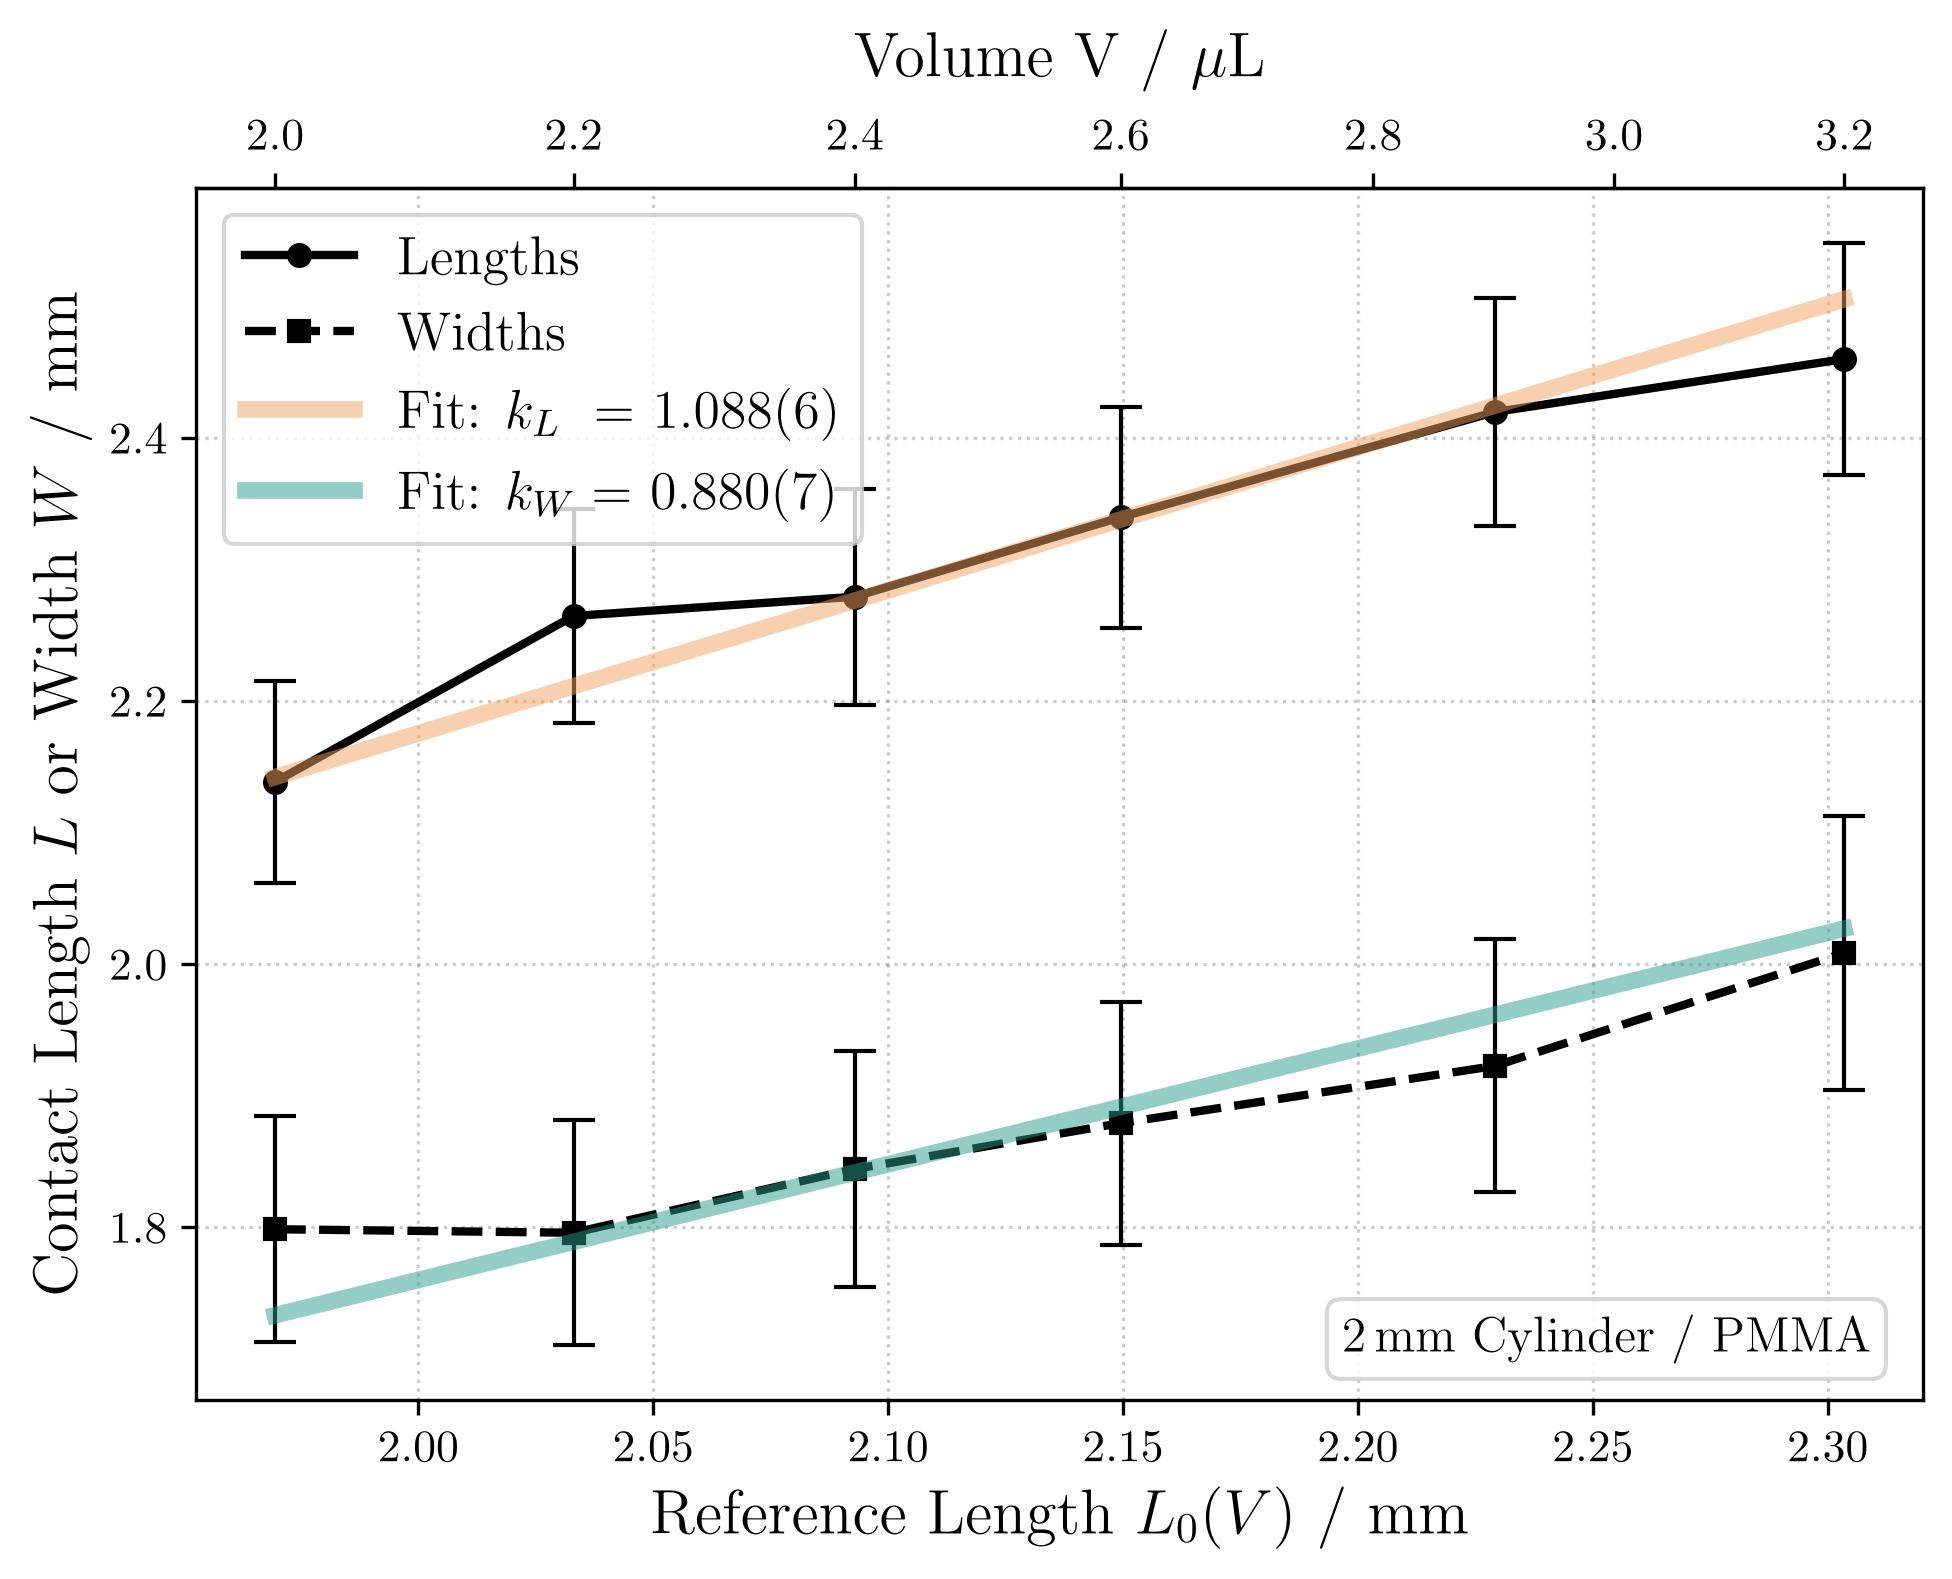
\includegraphics[width=0.55\linewidth]{../Plots/w06_02mm_PMMA_L+W_fit.jpg}
        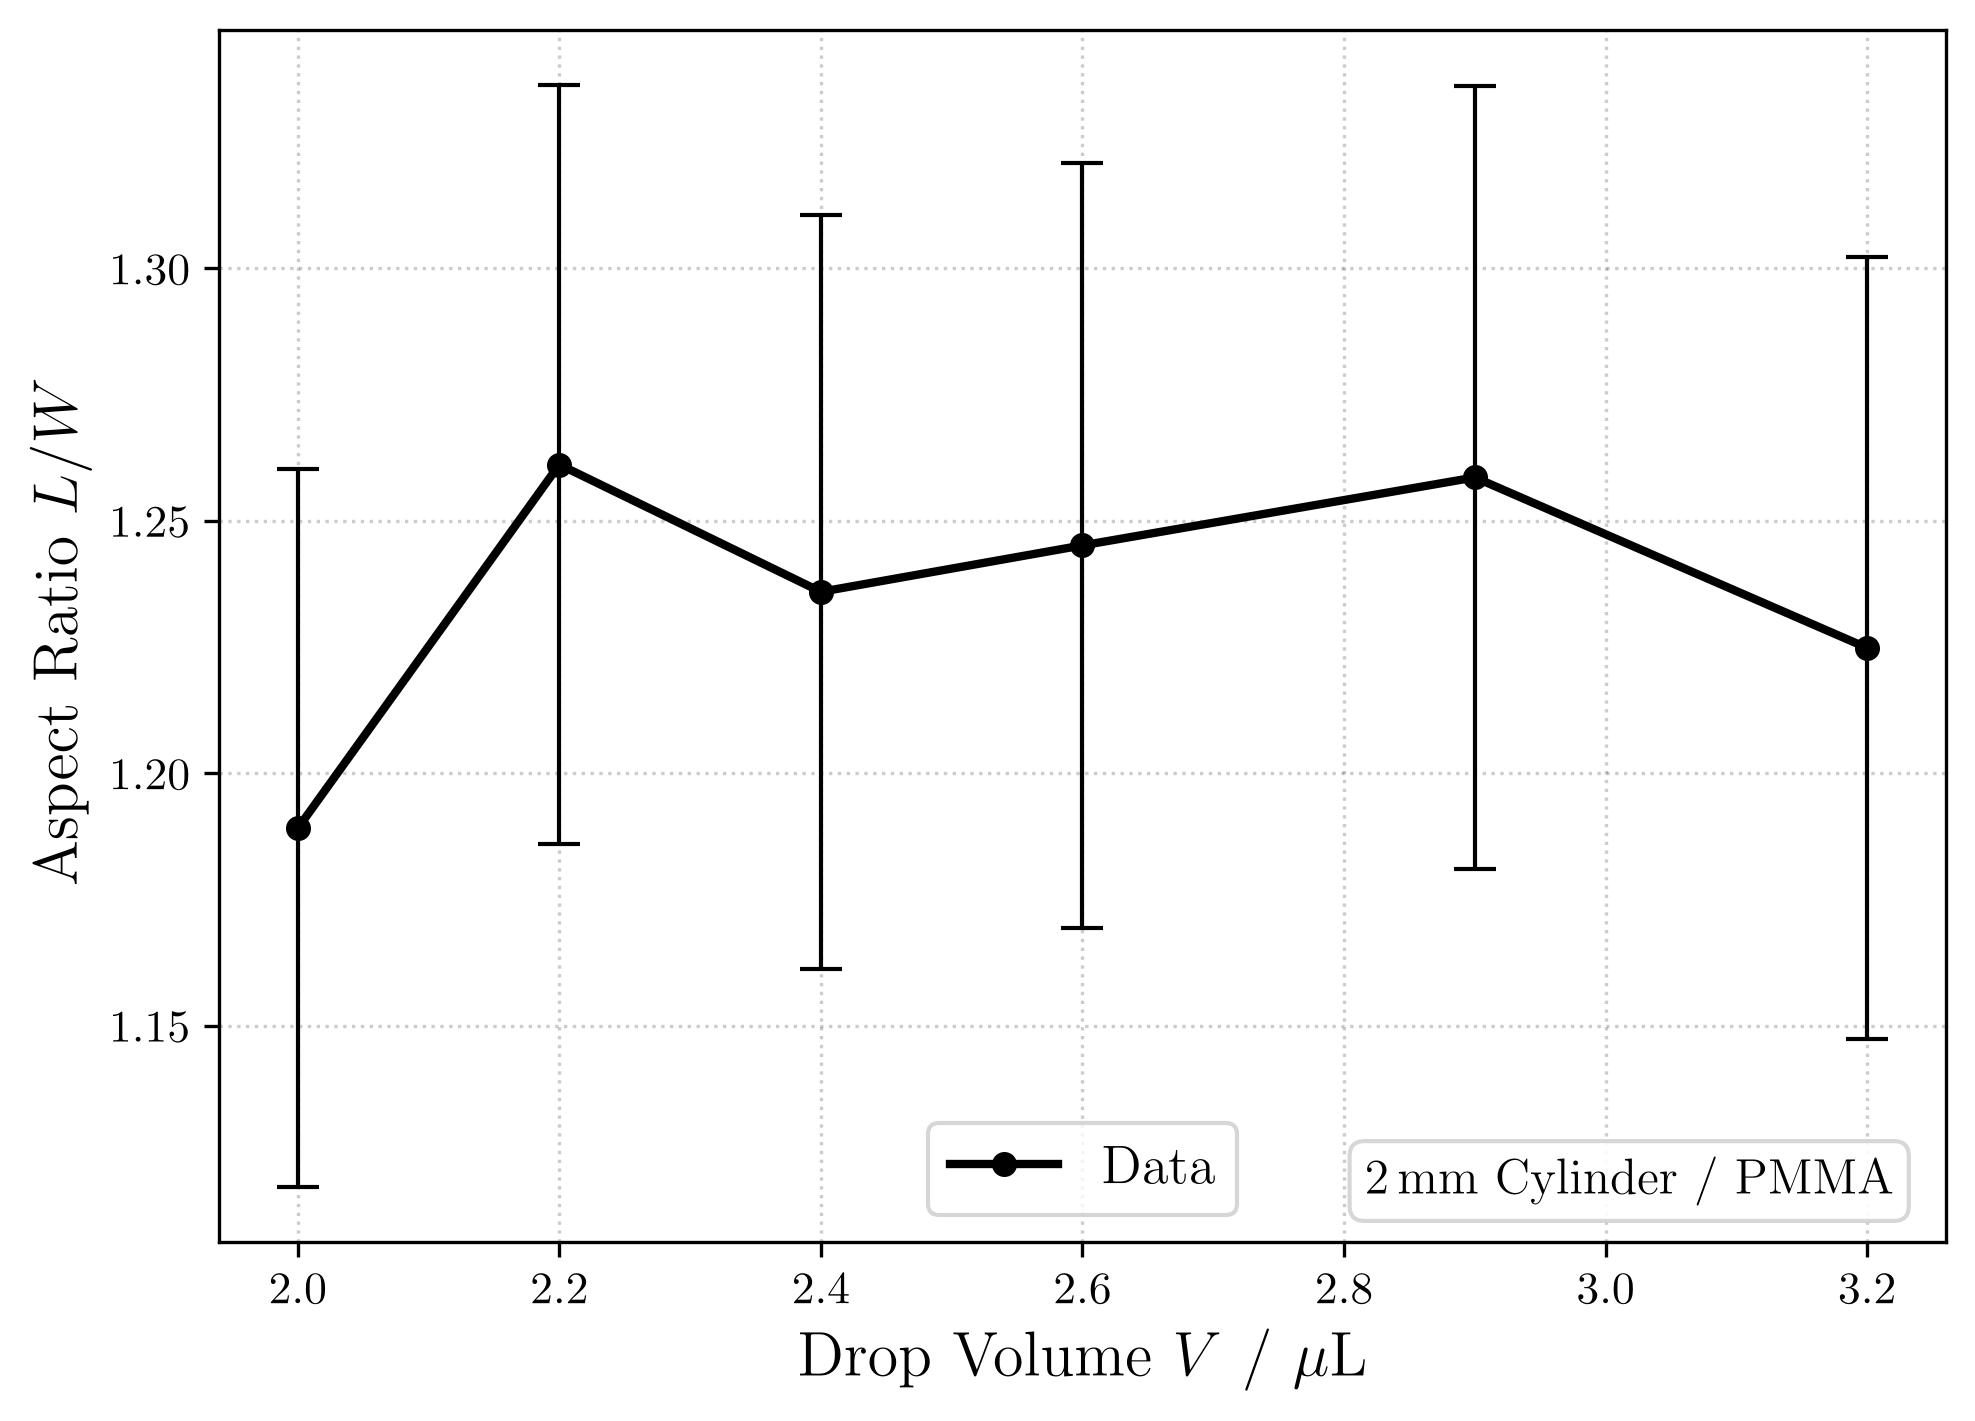
\includegraphics[width=0.55\linewidth]{../Plots/w06_02mm_PMMA_ratio.jpg}
        }
        \caption{Contact length and width against the reference length $L_0(V)$ with linear fits according to \cref{eq:L_and_W_against_L0} on the left. Even though the half-sphere model fits the data, $\chi^2 \ll 1$ suggest low significance. Their aspect ratios $L/W$ (right) on the \SI{2}{\milli\meter} PMMA cylinder does not deliver a clear result due to large uncertainties. }
        \label{fig:app:2mm_fit_ratio_PMMA}
    \end{figure}


% 4mm PMMA
    \begin{figure}[H]
        \centering
        \makebox[\textwidth]{        
        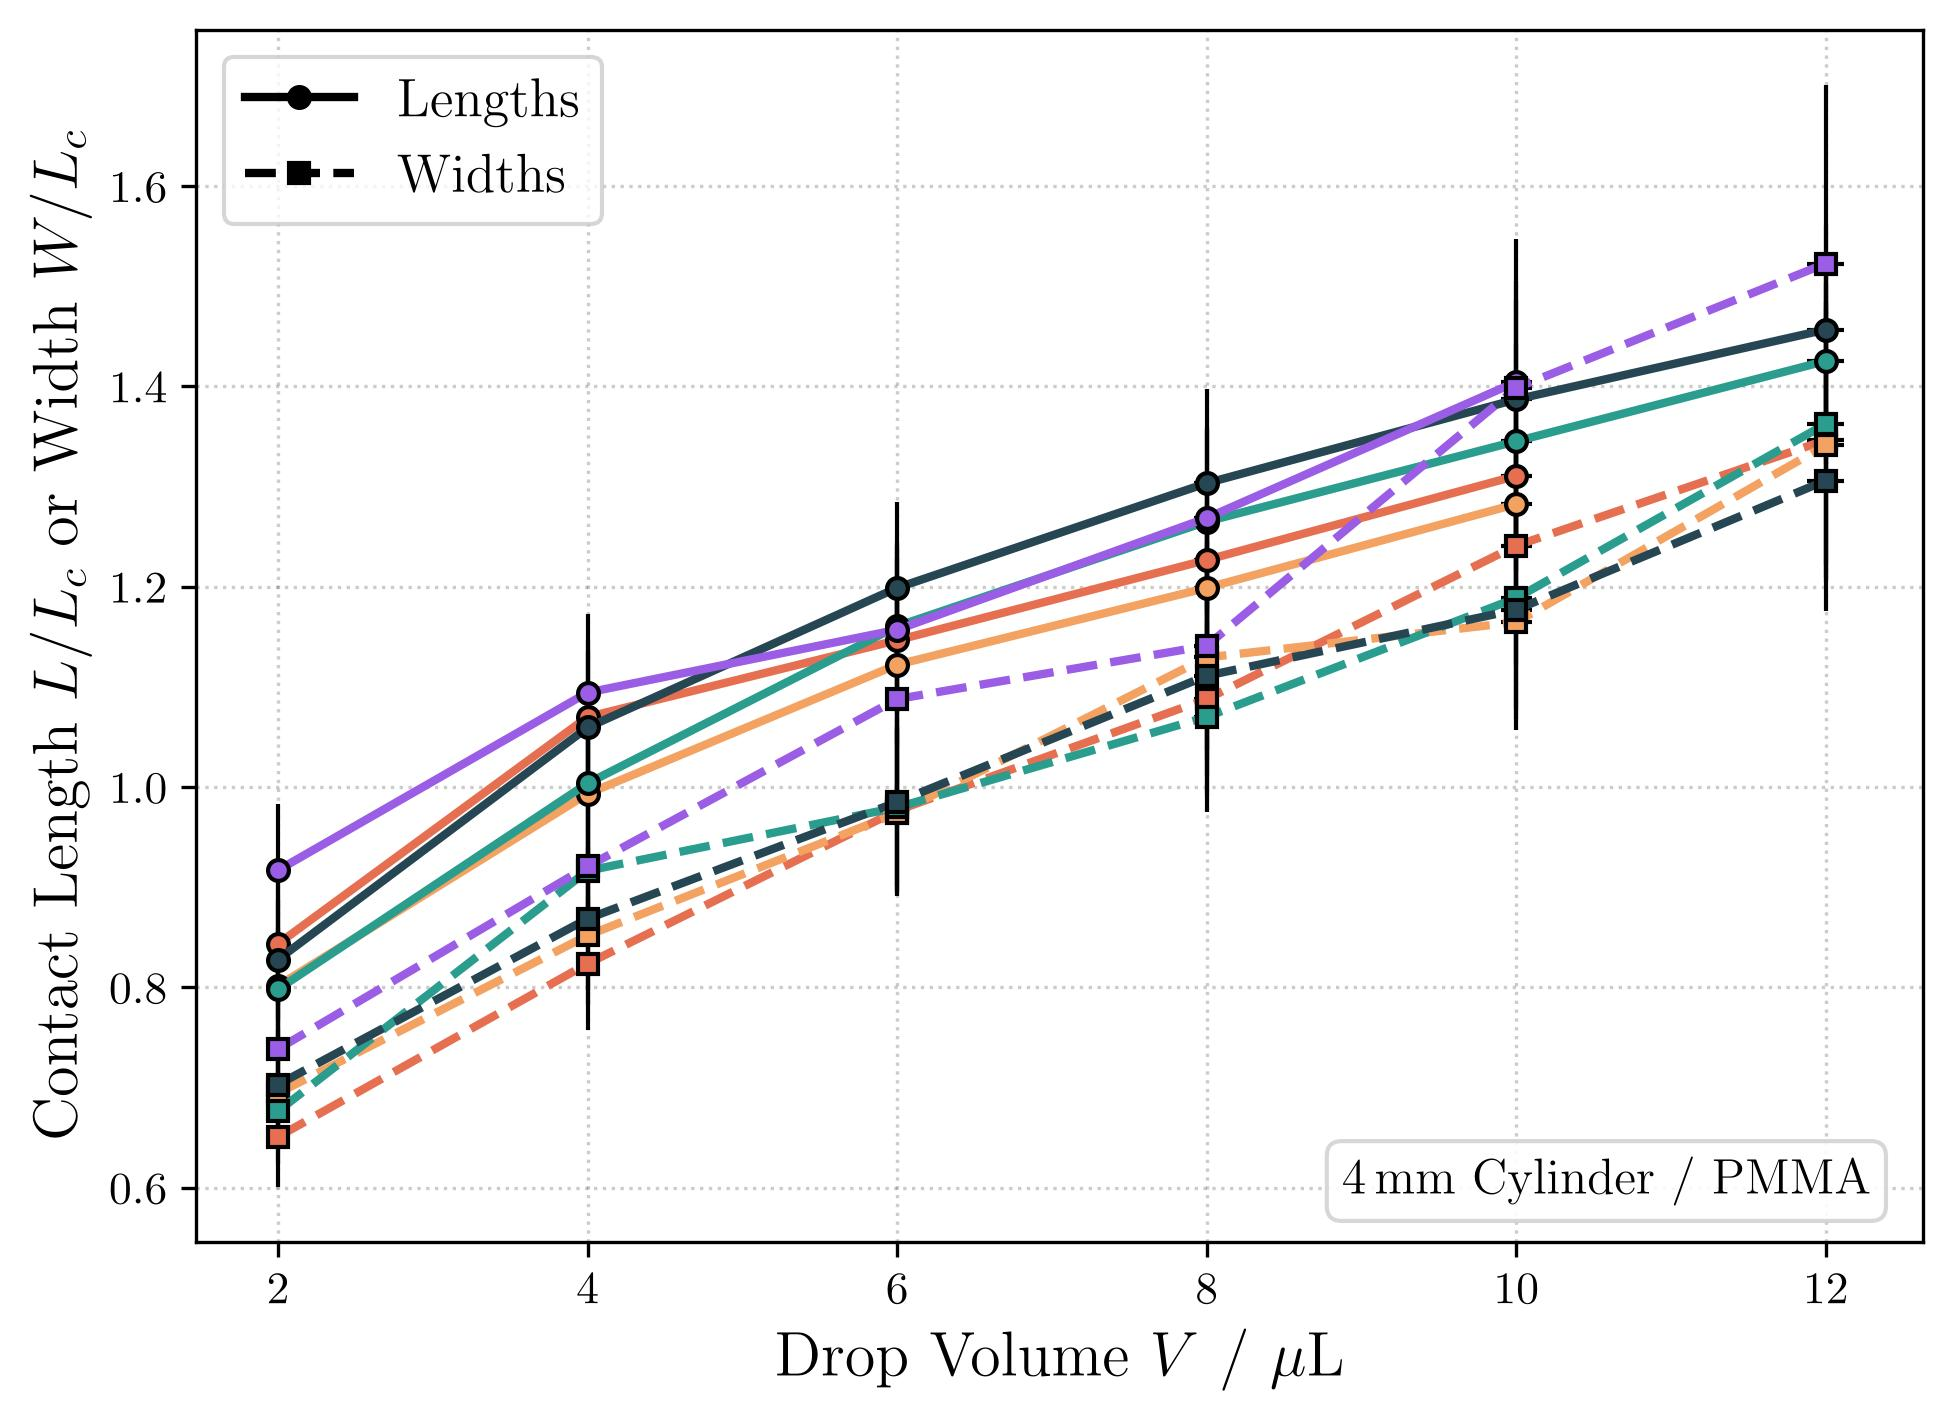
\includegraphics[width=0.55\linewidth]{../Plots/w06_04mm_PMMA_L+W.jpg}
        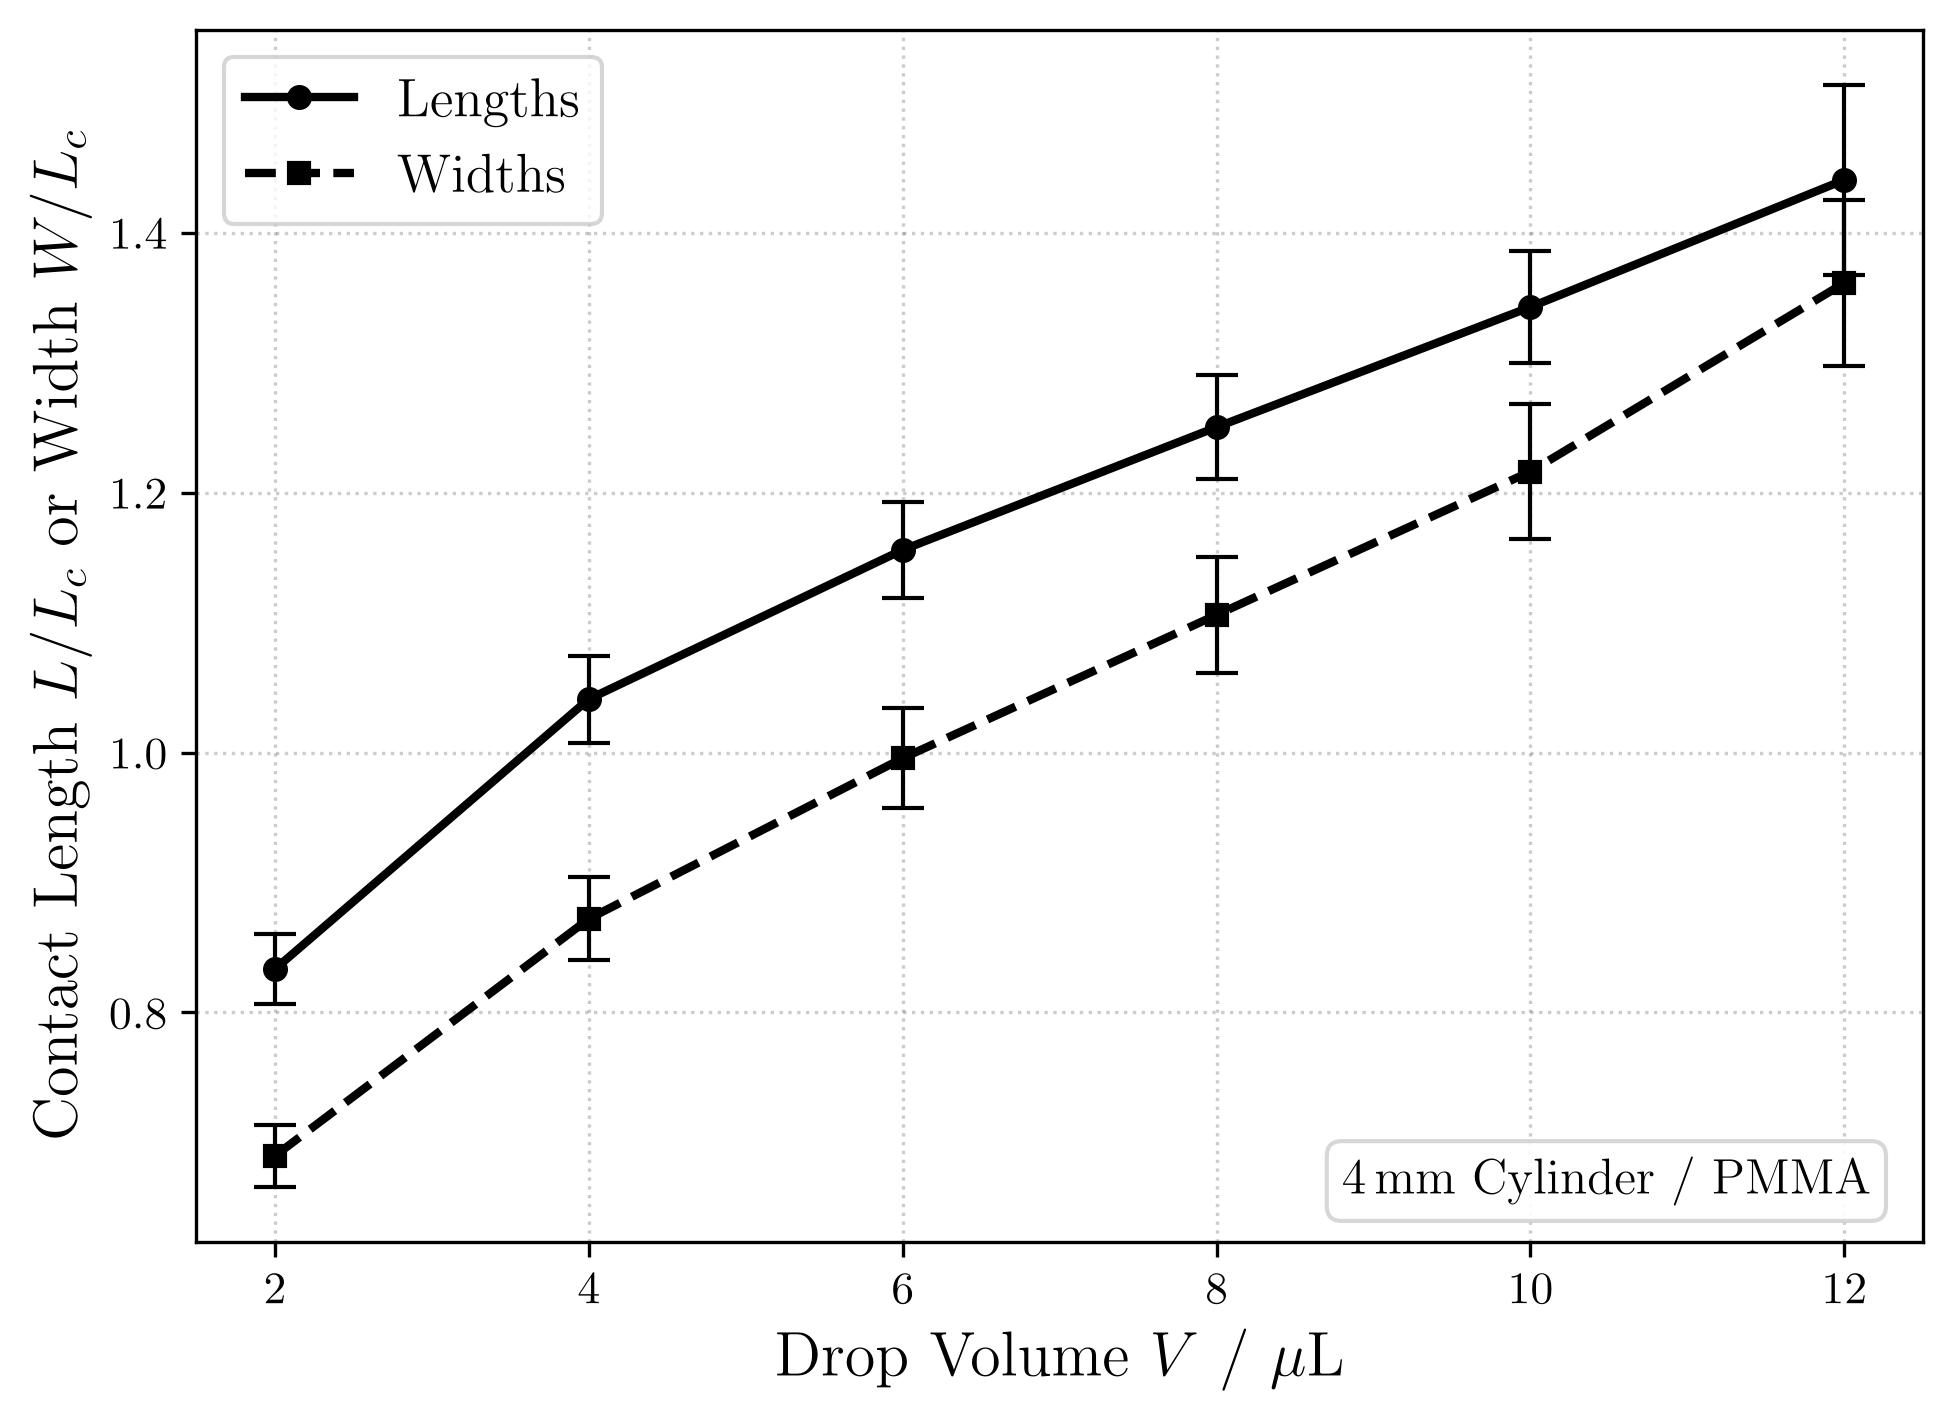
\includegraphics[width=0.55\linewidth]{../Plots/w06_04mm_PMMA_L+W_avg.jpg}
        }
        \caption{Measurements of contact length $L$ and width $W$ on the \SI{4}{\milli\meter} PMMA cylinder in raw (left) and averaged (right). Due to observed instability, the \SI{12}{\micro\liter} data points are not used in the analysis. $L$ and $W$ seem to converge, as gravity starts dominating over the surface tension for $L/L_c > 1$.}
        \label{fig:app:4mm_data_PMMA}
    \end{figure}

    \begin{figure}[H]
        \centering
        \makebox[\textwidth]{
        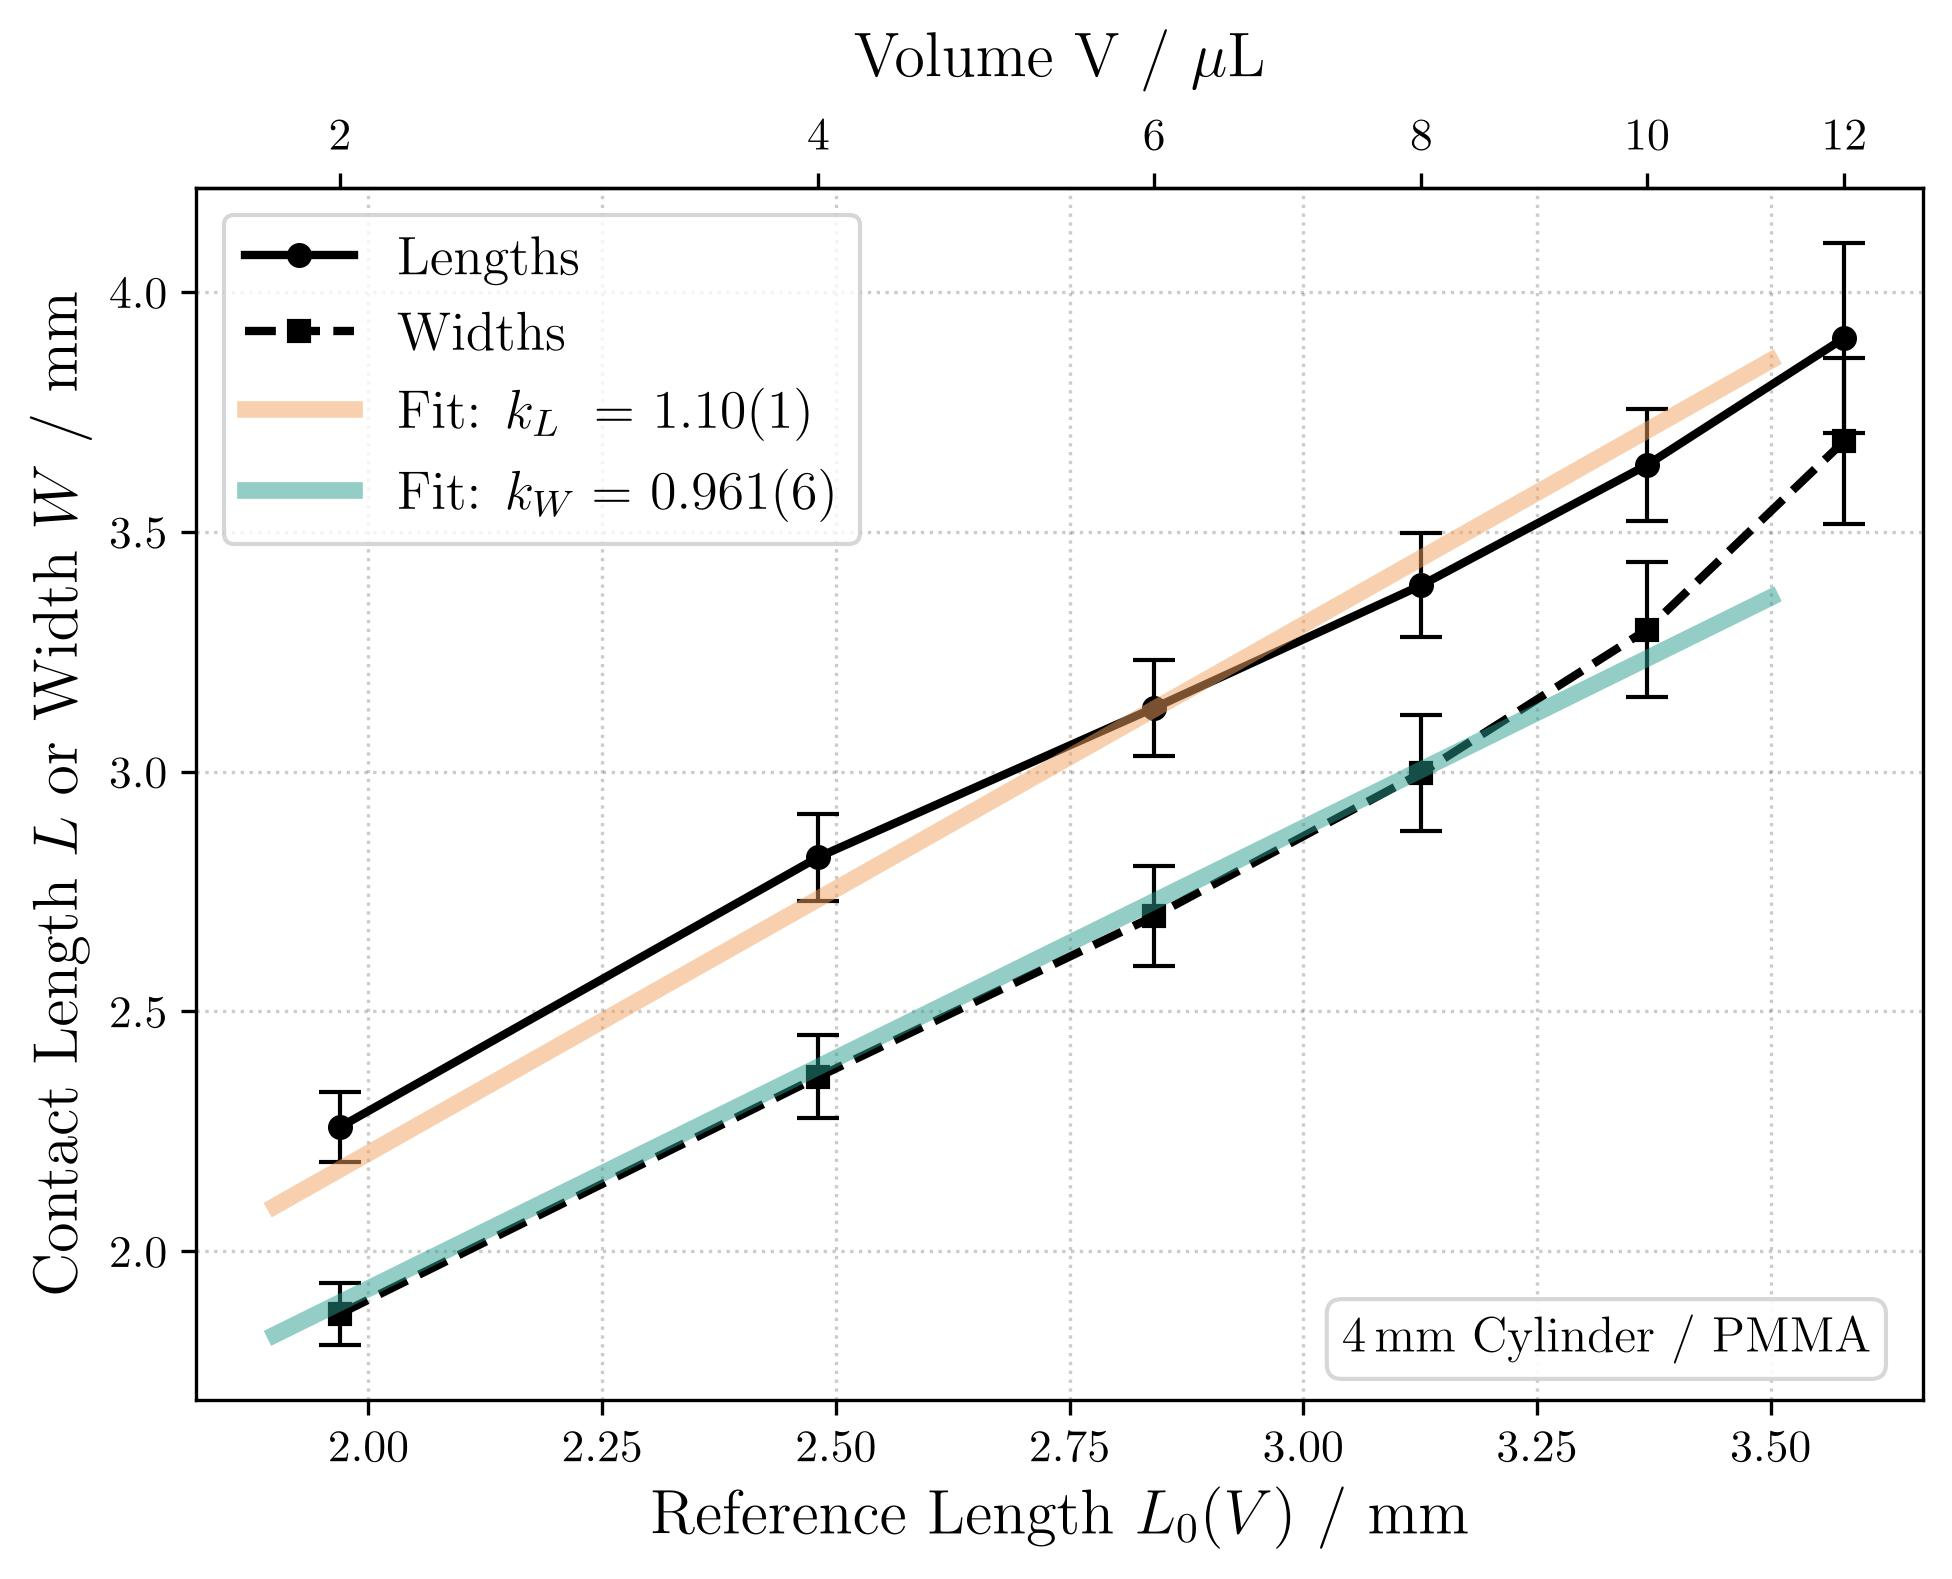
\includegraphics[width=0.55\linewidth]{../Plots/w06_04mm_PMMA_L+W_fit.jpg}
        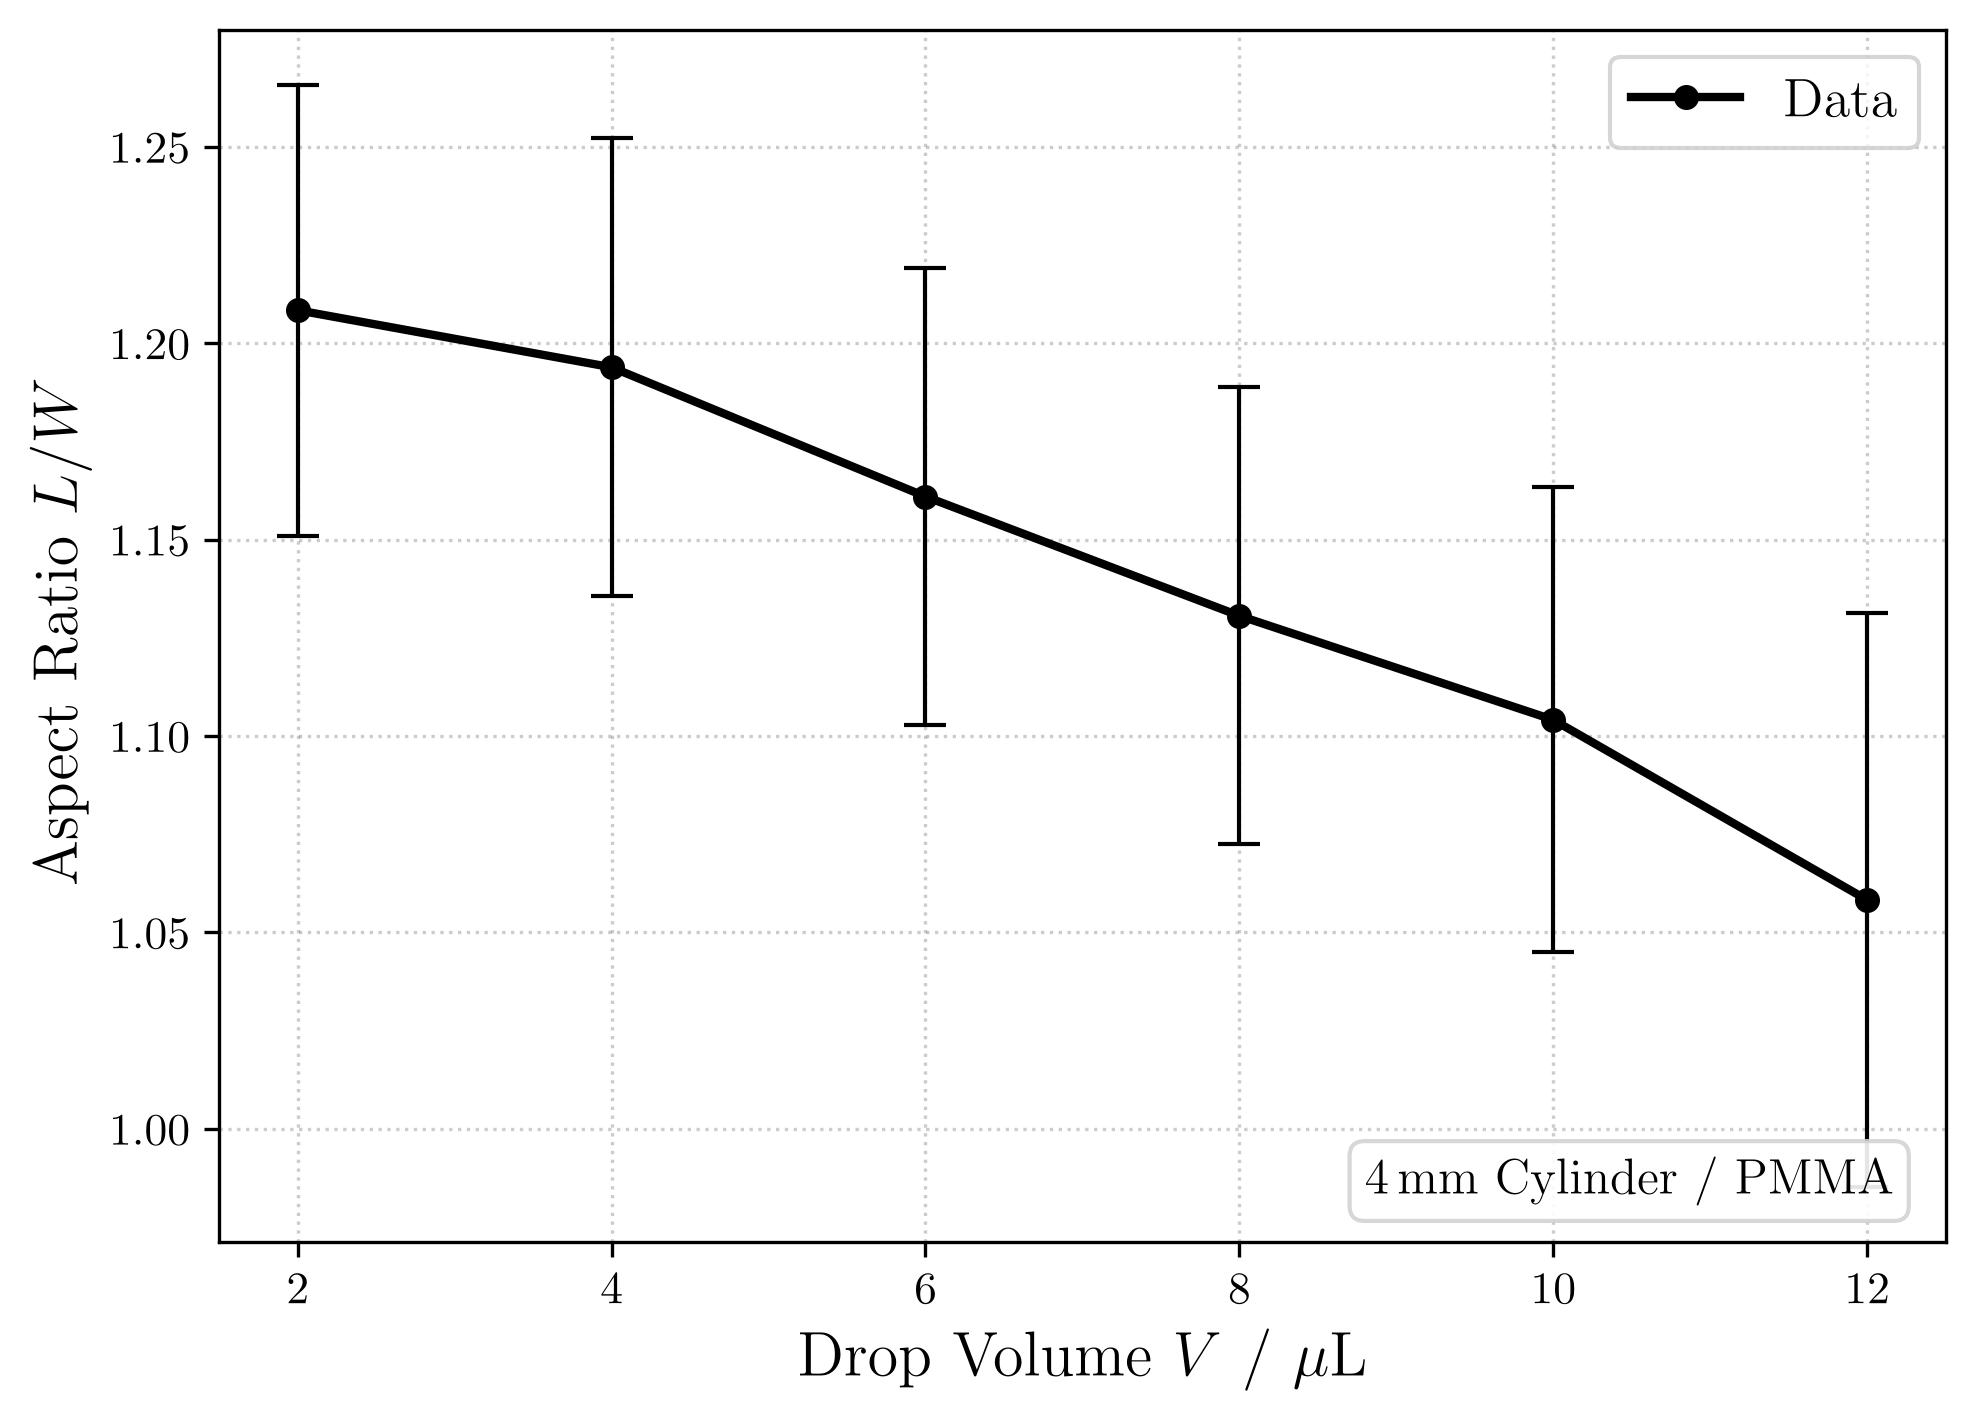
\includegraphics[width=0.55\linewidth]{../Plots/w06_04mm_PMMA_ratio.jpg}
        }
        \caption{Contact length and width against the reference length $L_0(V)$ with linear fits according to \cref{eq:L_and_W_against_L0} on the left. Again, the linear model is confirmed with high flexibility $(\chi^2 \ll 1)$ and $L > W$ for all $V$. Their aspect ratios $L/W$ (right) on the \SI{4}{\milli\meter} PMMA cylinder trends visibly down to $1$, where the droplet width will exceed its length.}
        \label{fig:app:4mm_fit_ratio_PMMA}
    \end{figure}


% 10mm PMMA
    \begin{figure}[H]
        \centering
        \makebox[\textwidth]{
        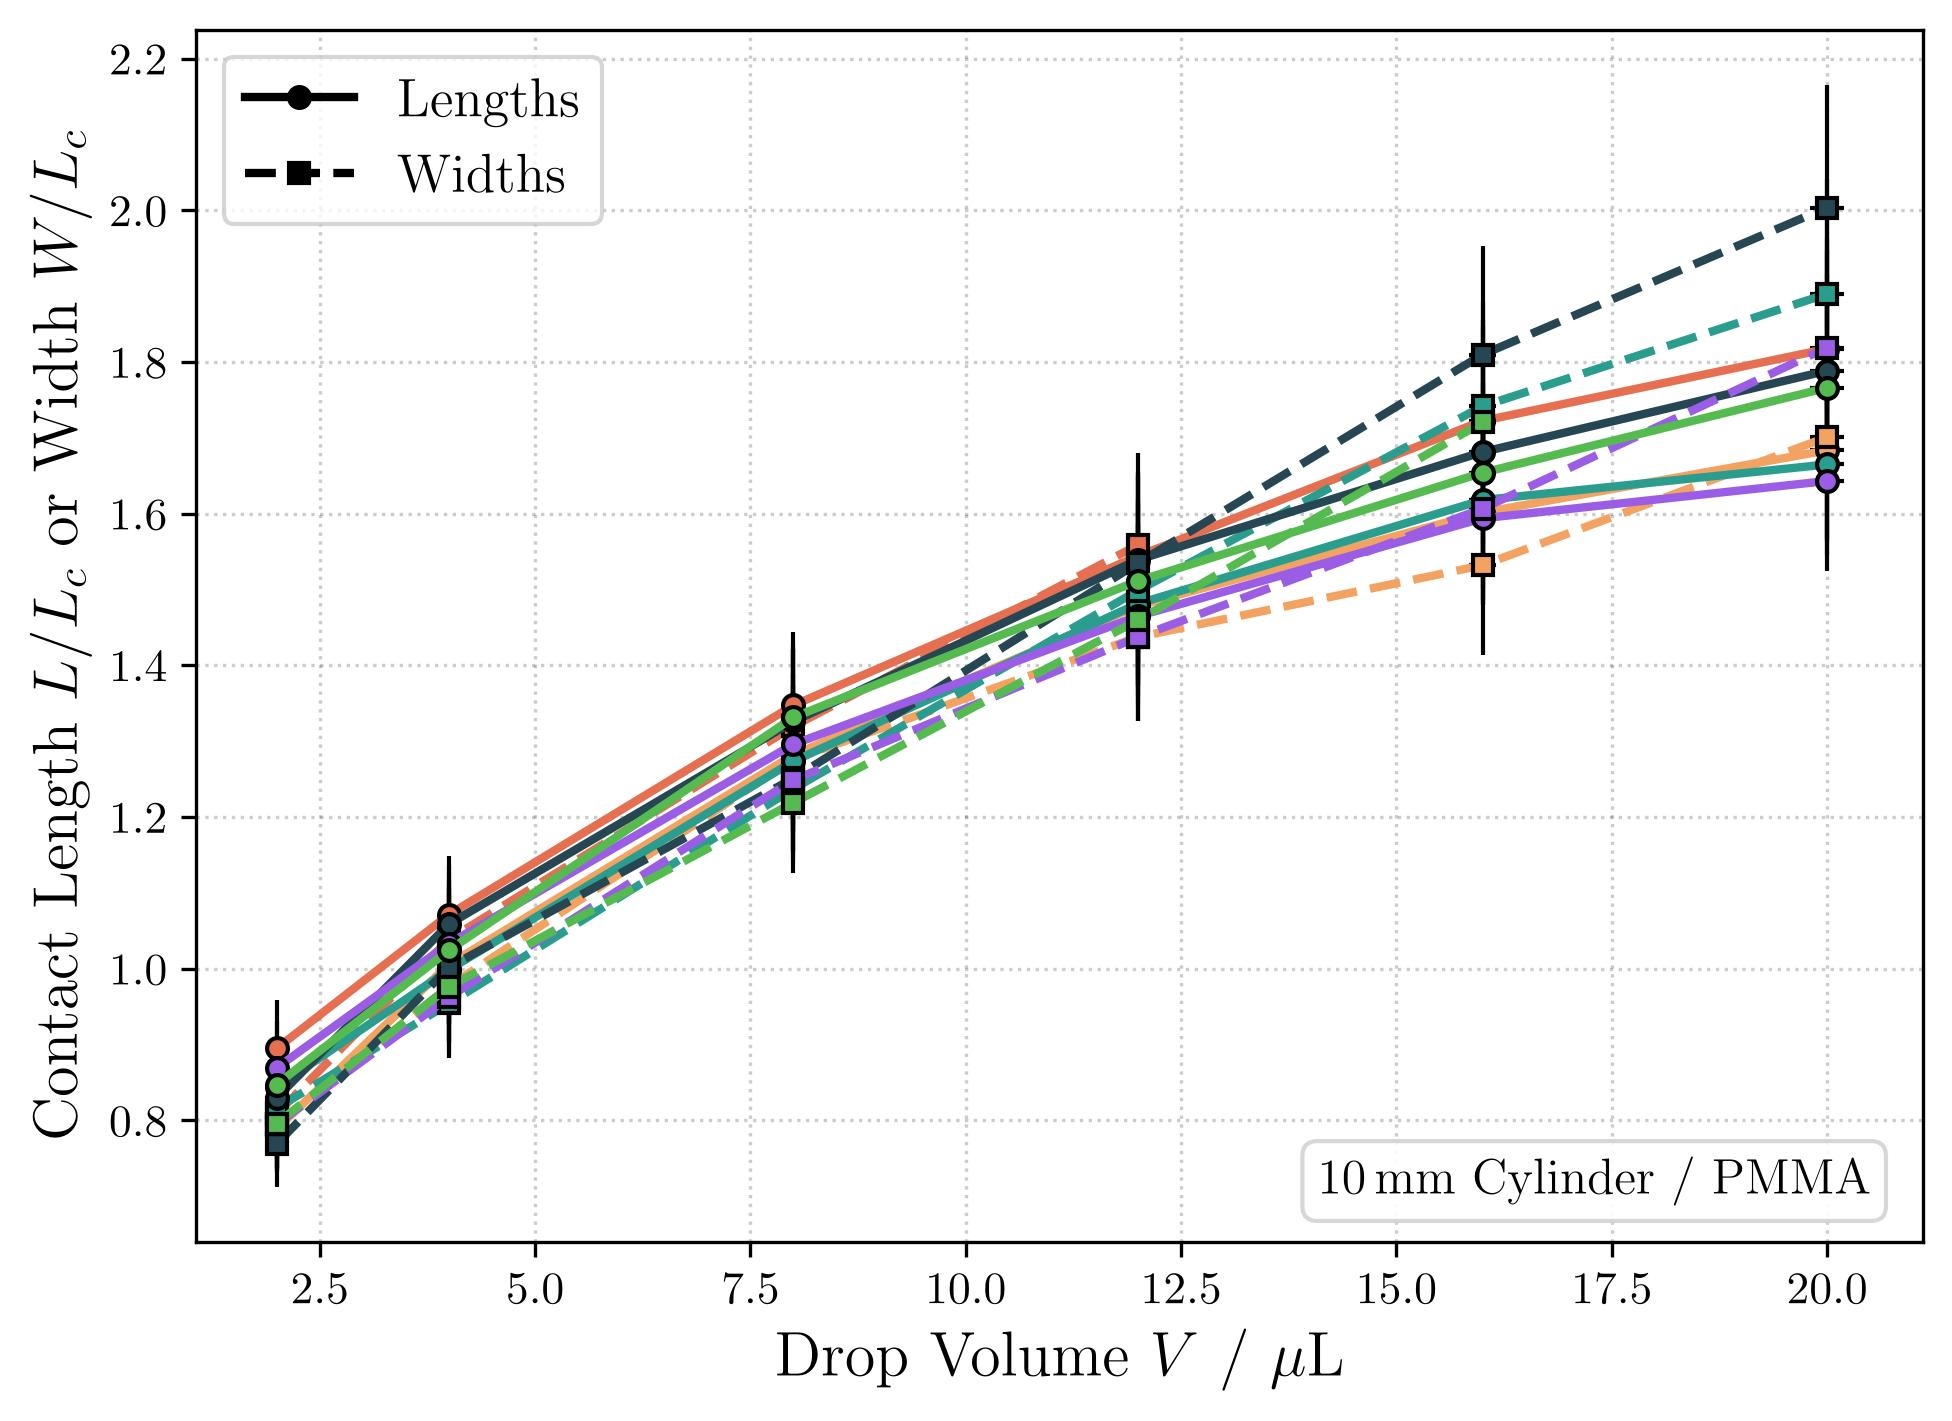
\includegraphics[width=0.55\linewidth]{../Plots/w06_10mm_PMMA_L+W.jpg}
        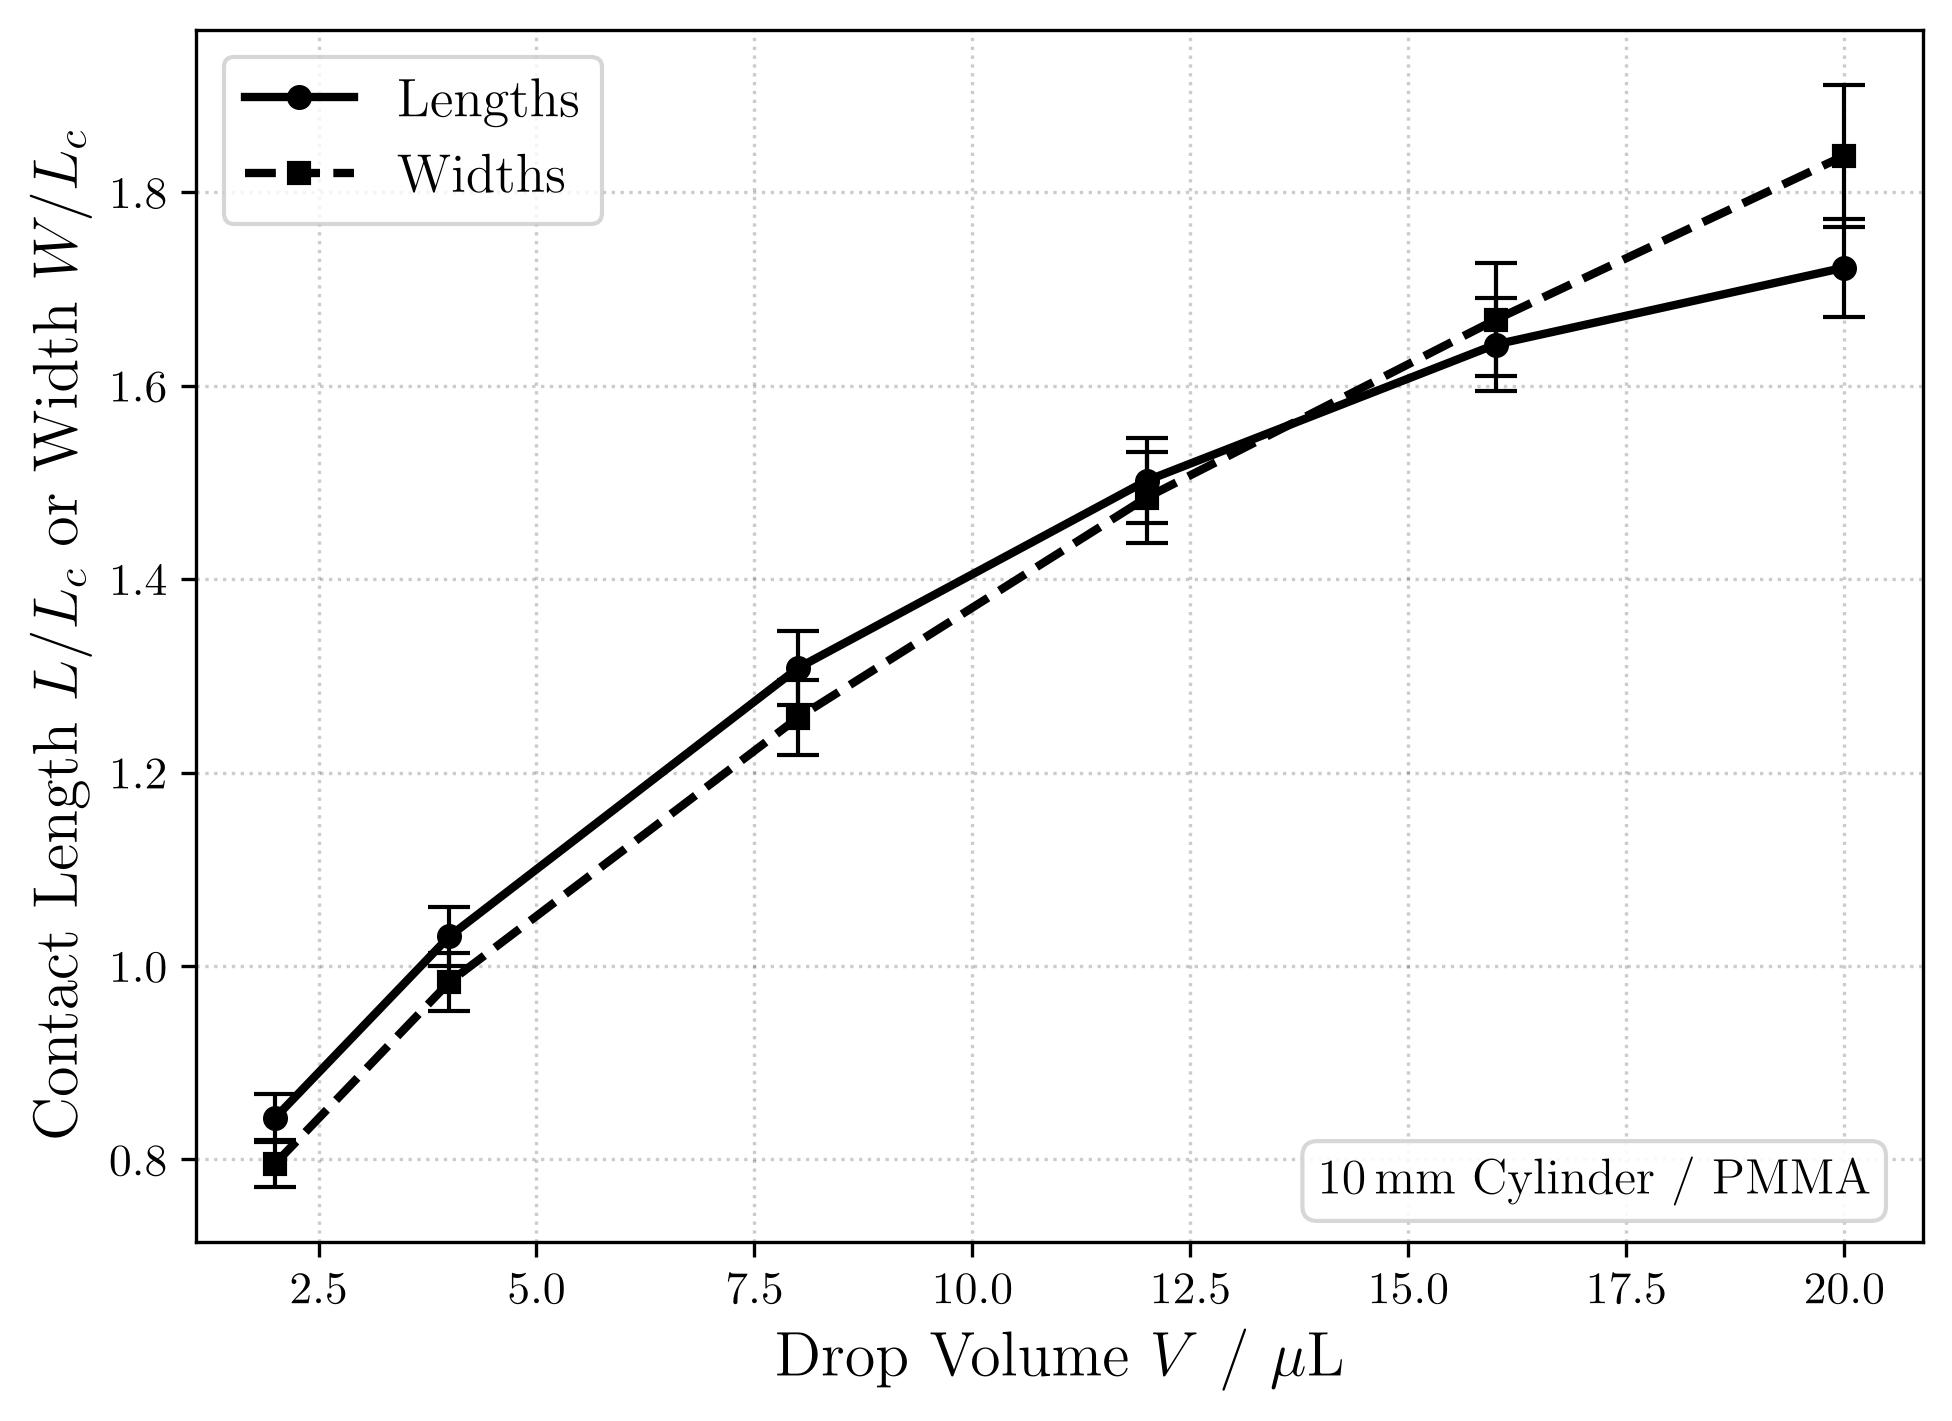
\includegraphics[width=0.55\linewidth]{../Plots/w06_10mm_PMMA_L+W_avg.jpg}
        }
        \caption{Measurements of contact length $L$ and width $W$ on the \SI{10}{\milli\meter} PMMA cylinder in raw (left) and averaged (right). The length $L$ is overtaking by the width $W$ at \SI{13.5}{\micro\liter}, indicating the domination of gravity over surface tension $(L/L_c > 1.5)$. Due to observed instability, the \SI{20}{\micro\liter} data points are not used in the quantitative analysis.}
        \label{fig:app:10mm_data_PMMA}
    \end{figure}

    \begin{figure}[H]
        \centering
        \makebox[\textwidth]{
        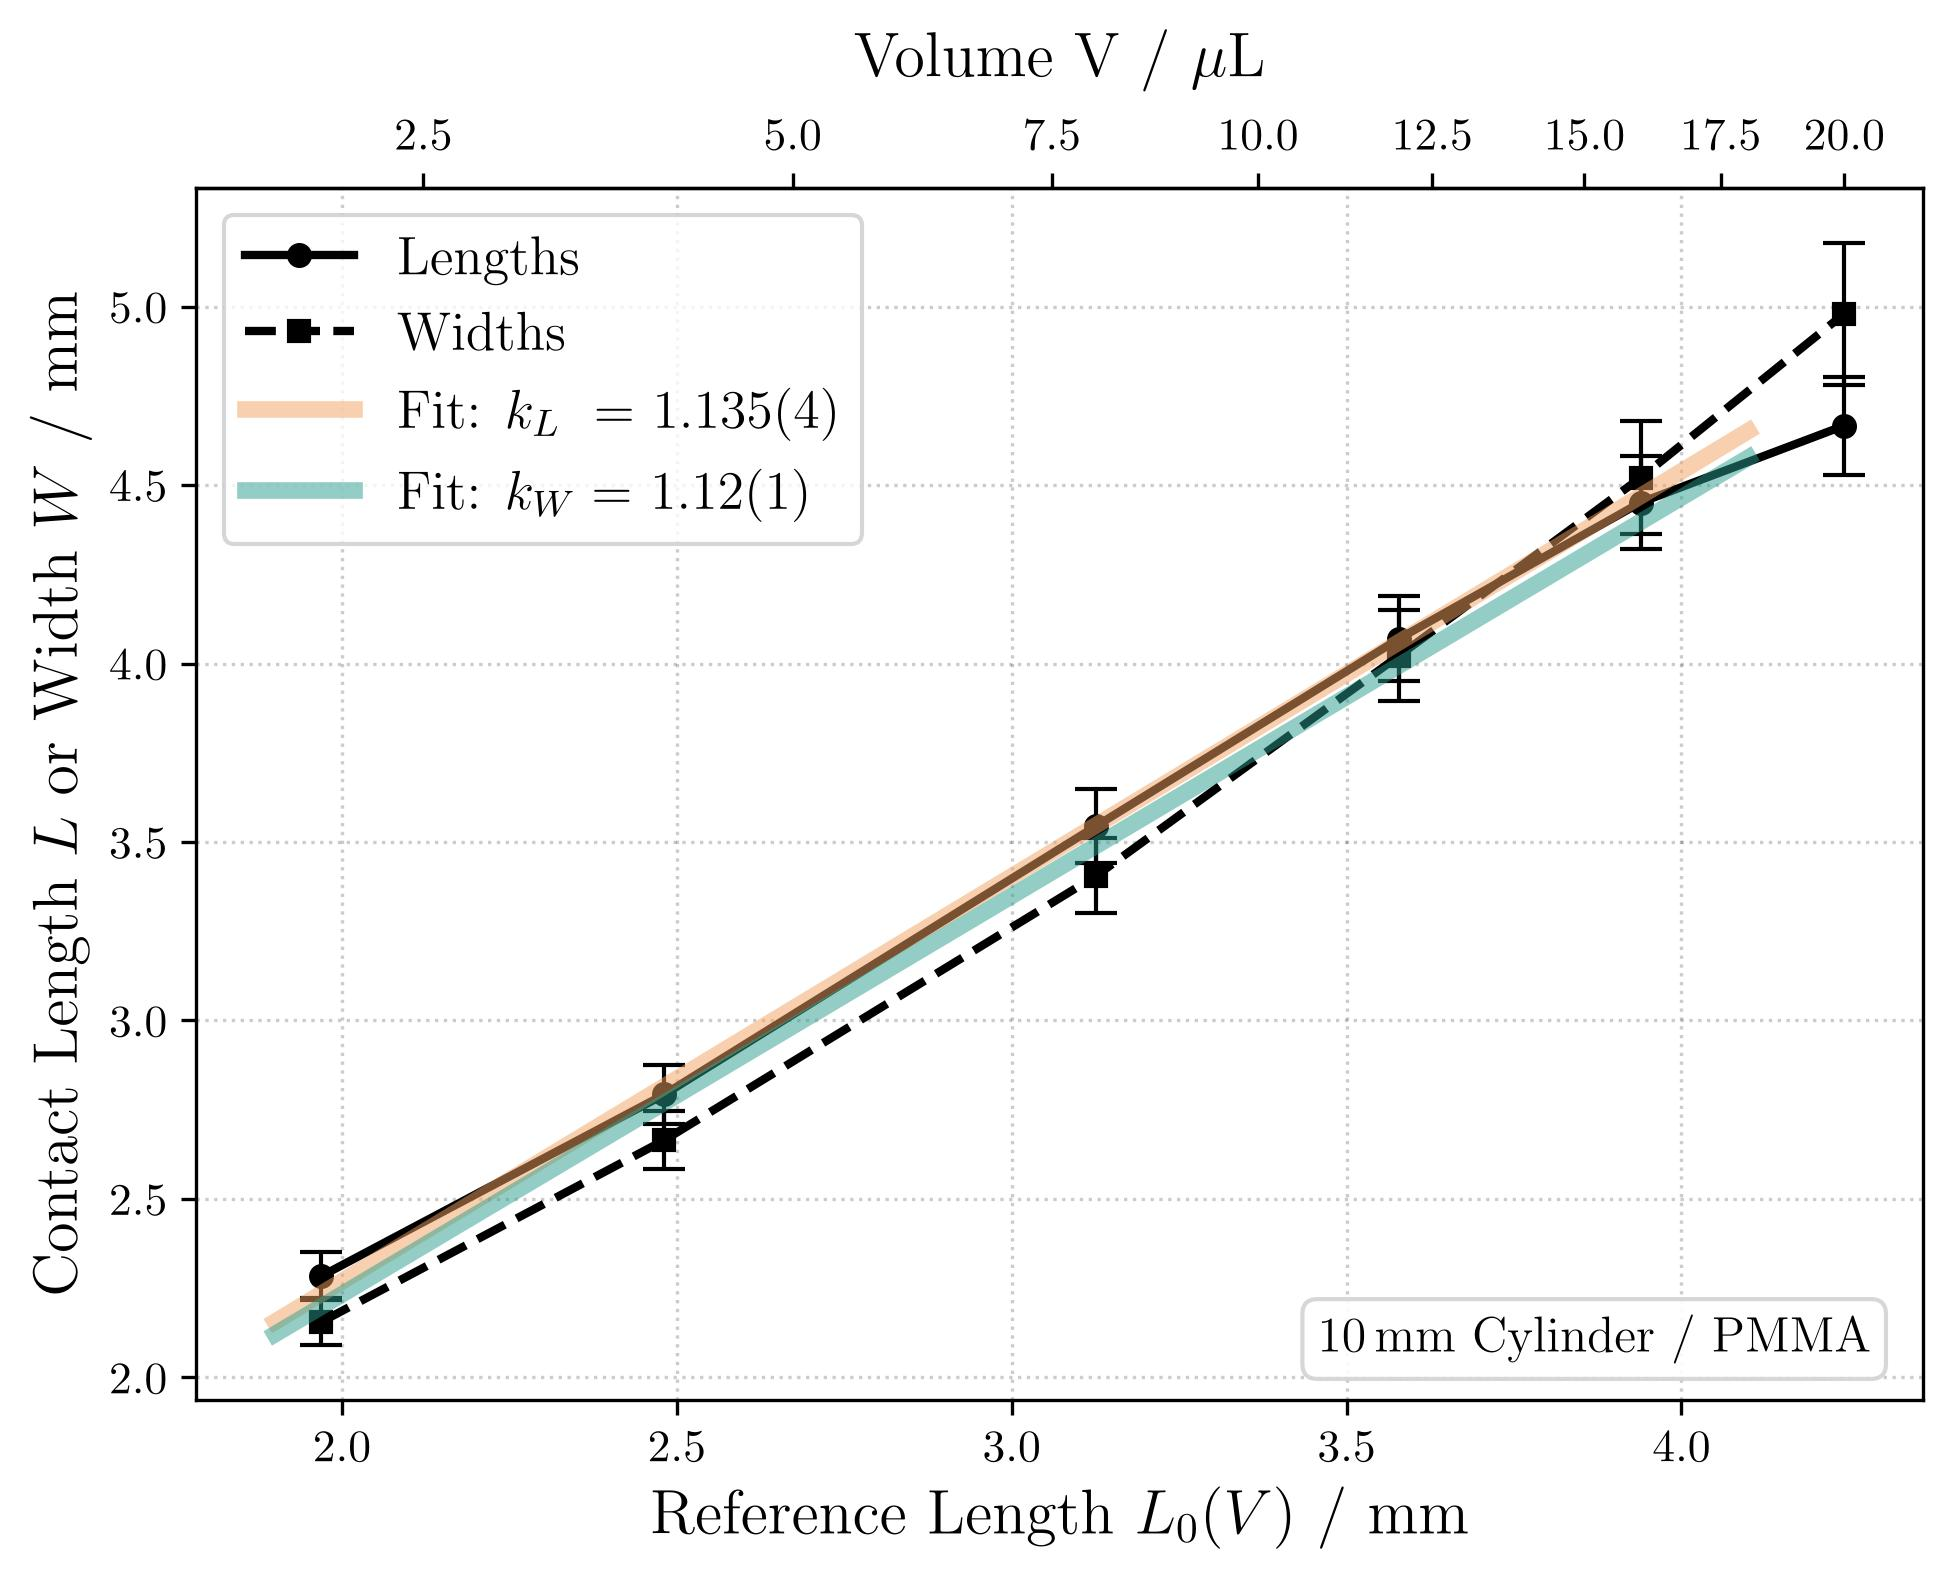
\includegraphics[width=0.55\linewidth]{../Plots/w06_10mm_PMMA_L+W_fit.jpg}
        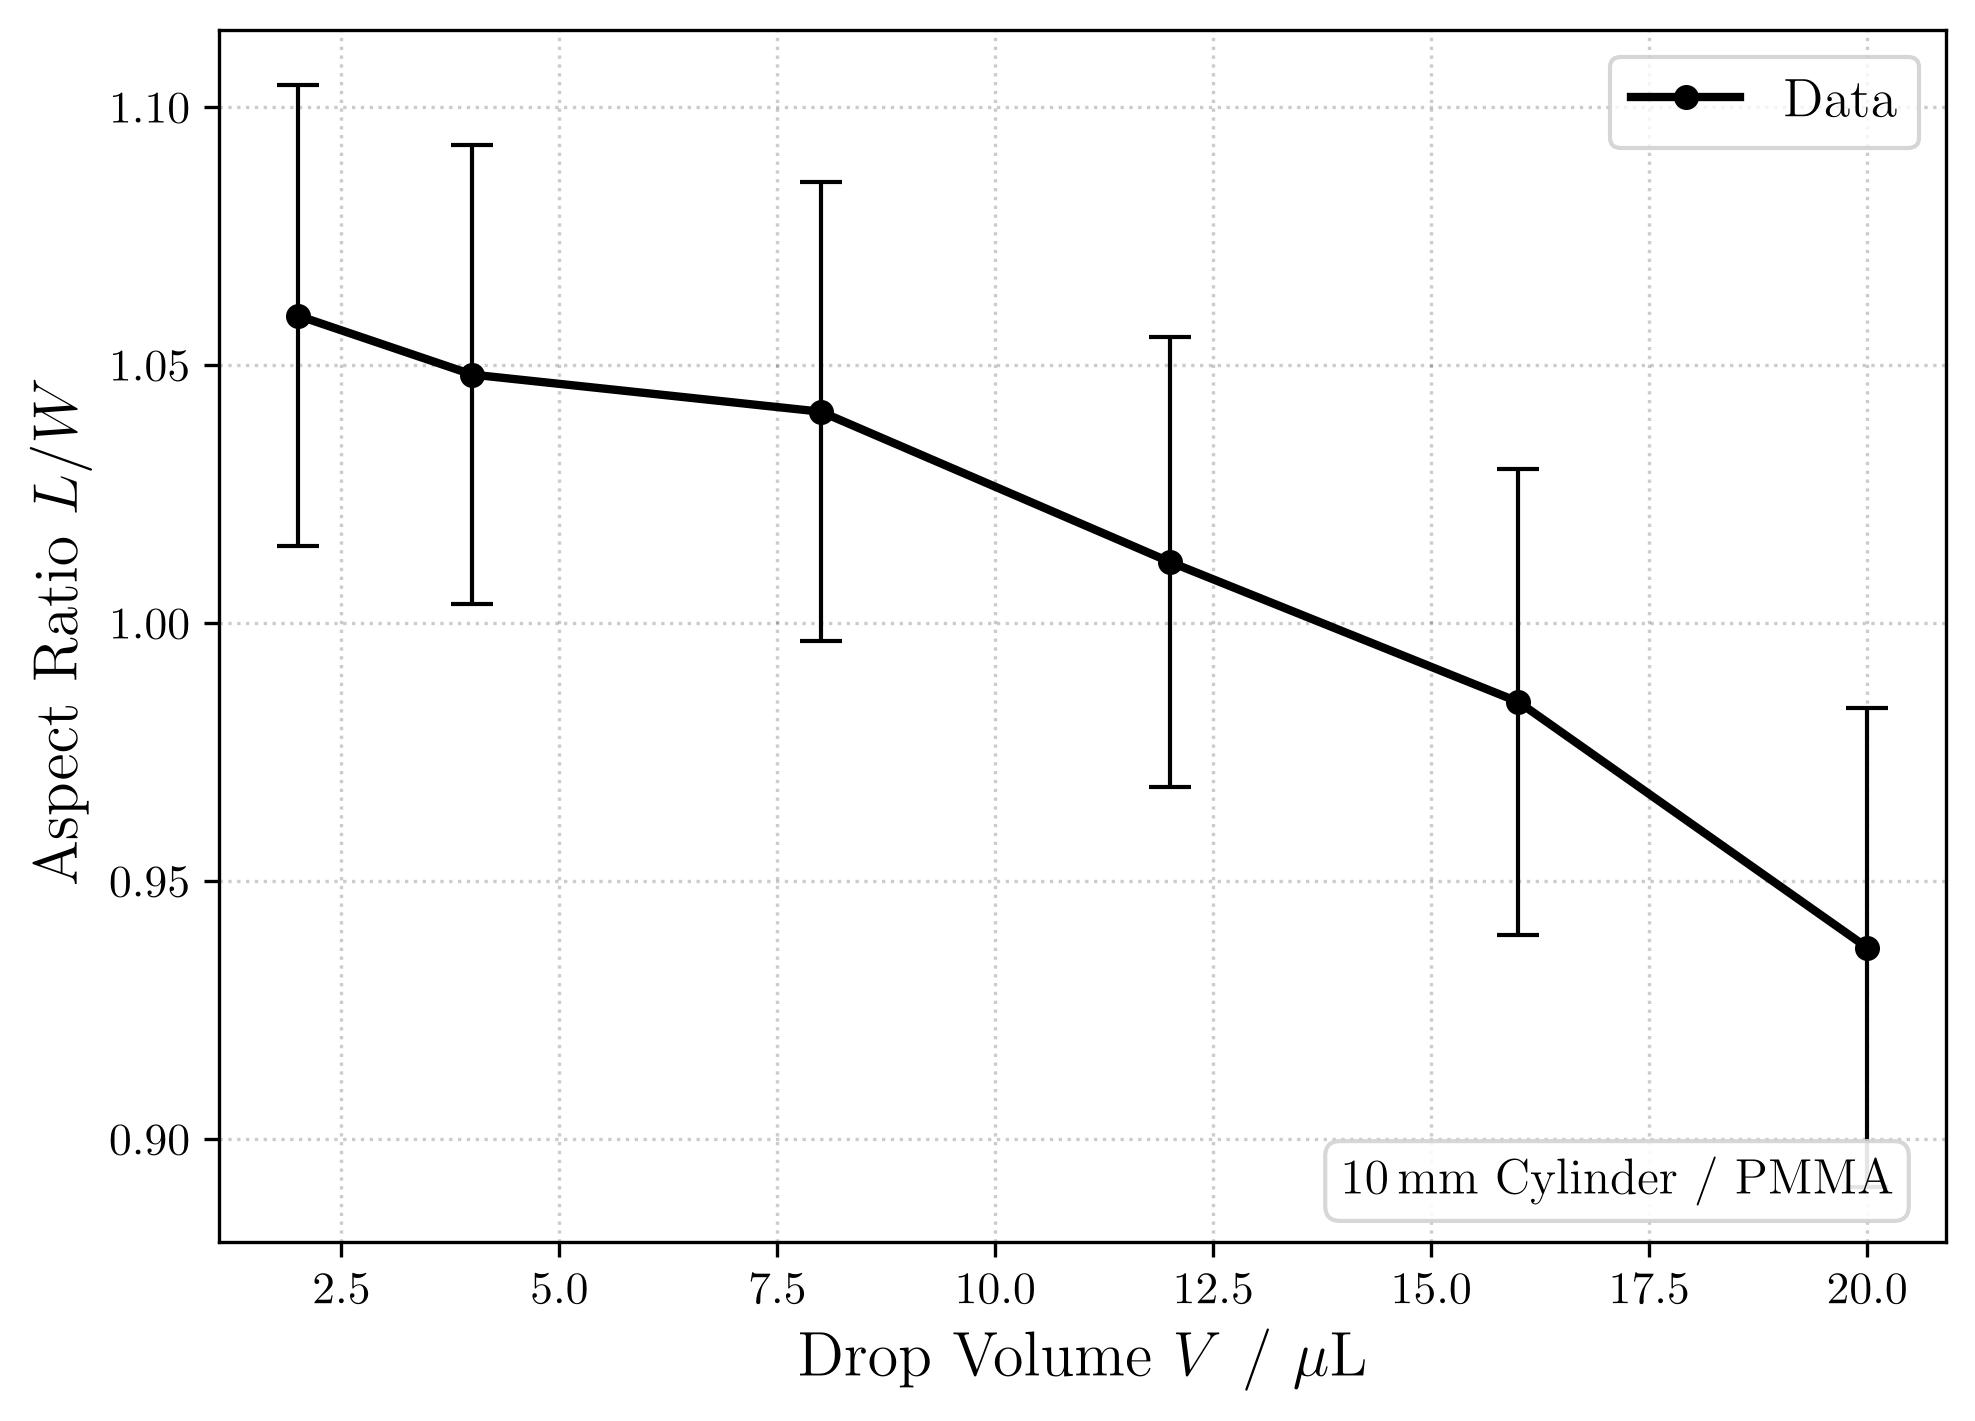
\includegraphics[width=0.55\linewidth]{../Plots/w06_10mm_PMMA_ratio.jpg}
        }
        \caption{Contact length and width against the reference length $L_0(V)$ with linear fits according to \cref{eq:L_and_W_against_L0} on the left. As before, the linear model is confirmed with high flexibility $(\chi^2 \ll 1)$ and $k_L$ , $k_W > 1$ indicates the \enquote{rounded} drop geometry. Their aspect ratios $L/W$ (right) on the \SI{10}{\milli\meter} PMMA cylinder confirm the overtaking of gravity through the decrease in $L/W$ down to below $0.95$.  }
        \label{fig:app:10mm_fit_ratio_PMMA}
    \end{figure}


% flat PMMA
    \begin{figure}[H]
        \centering
        \makebox[\textwidth]{
        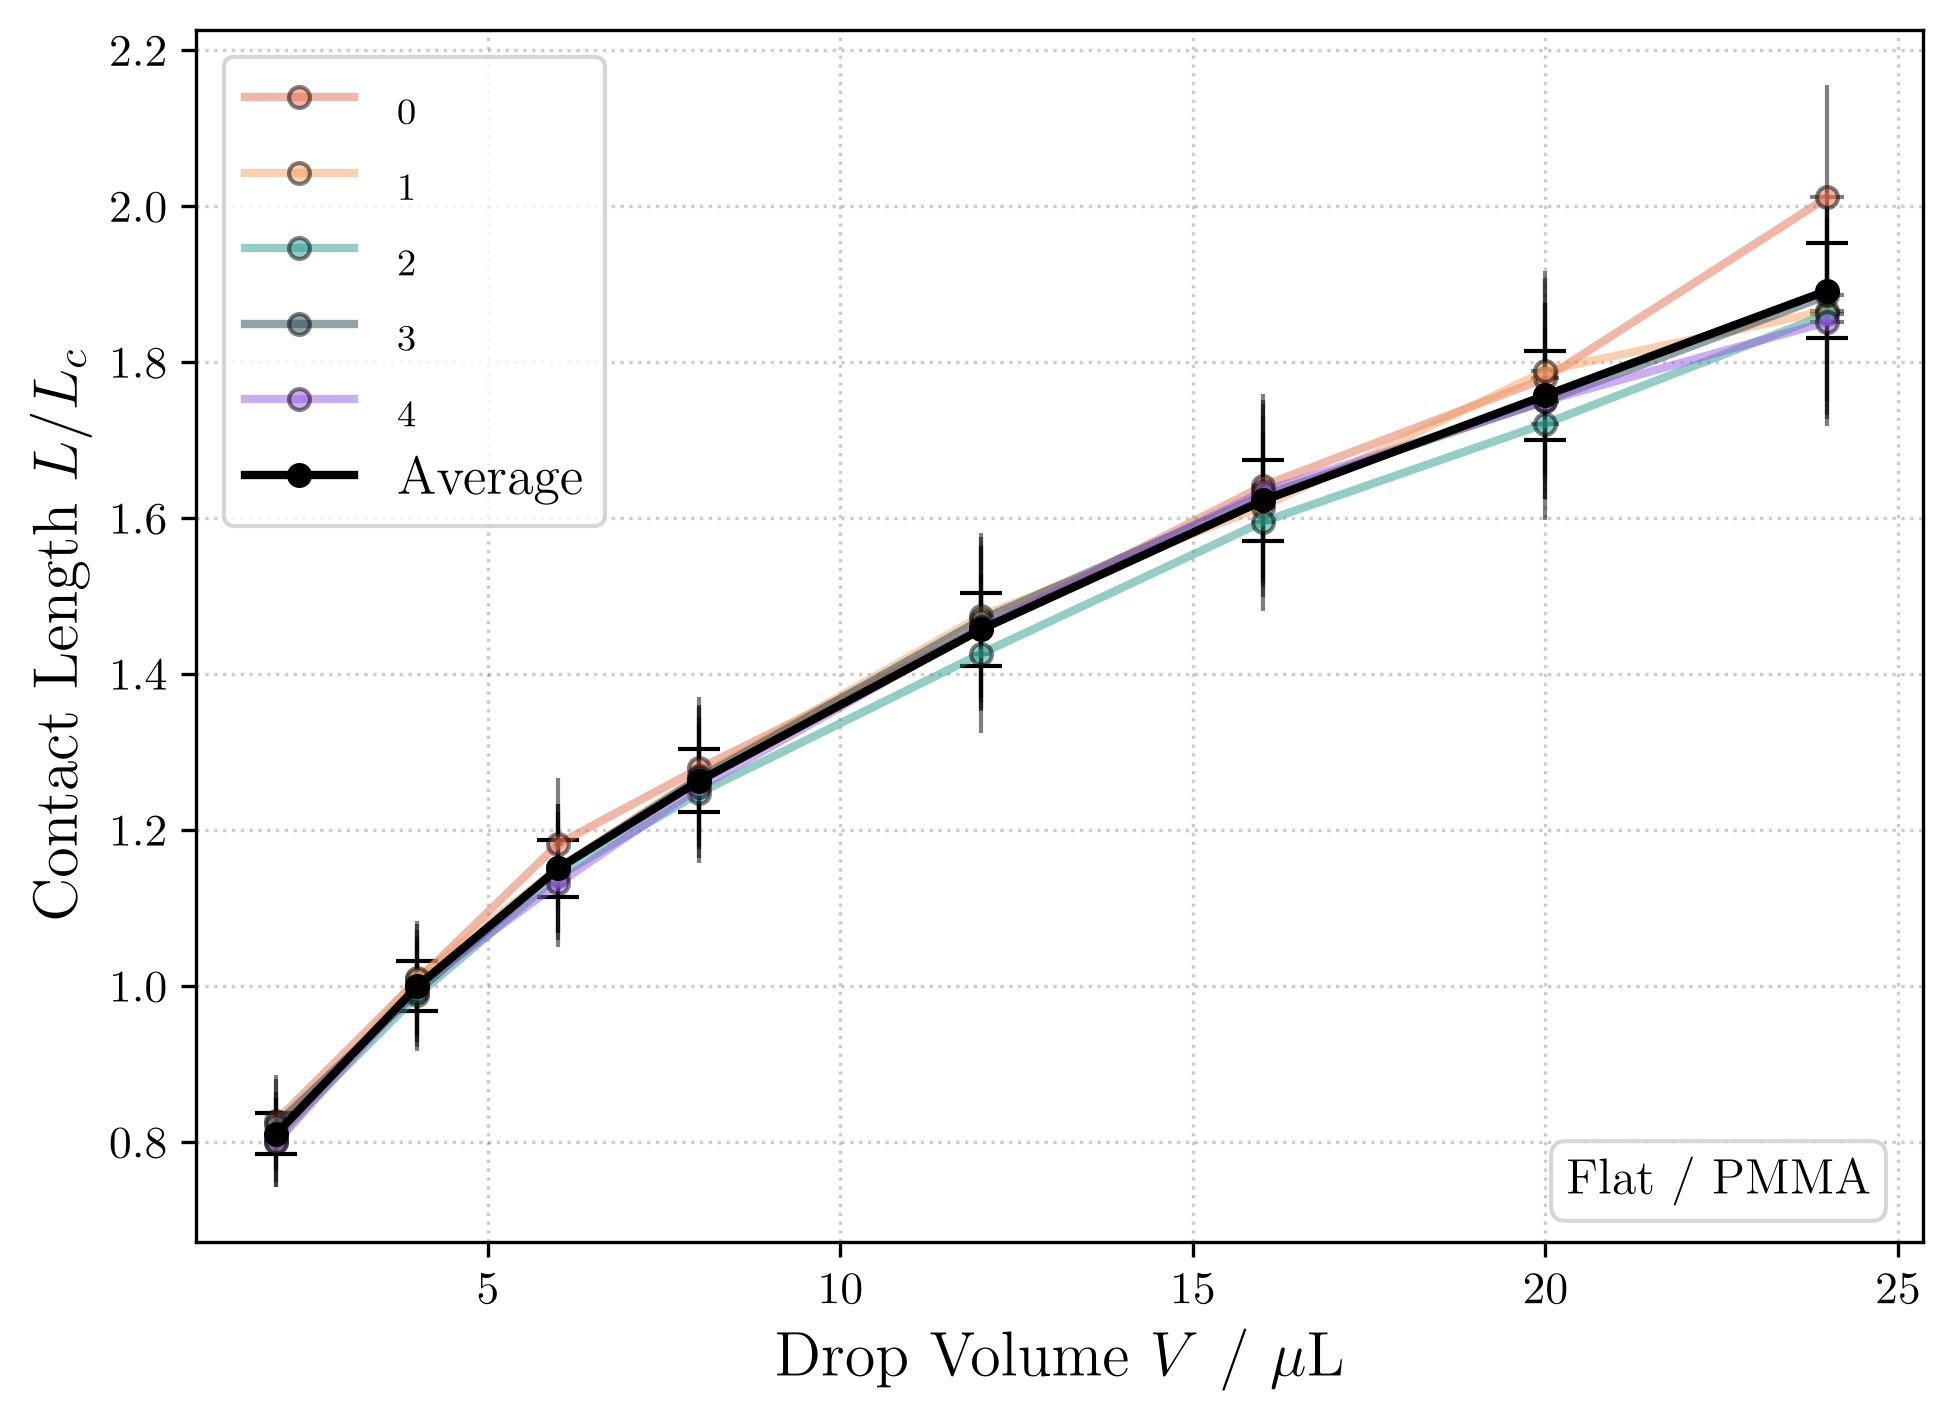
\includegraphics[width=0.55\linewidth]{../Plots/w06_flat_PMMA_L.jpg}
        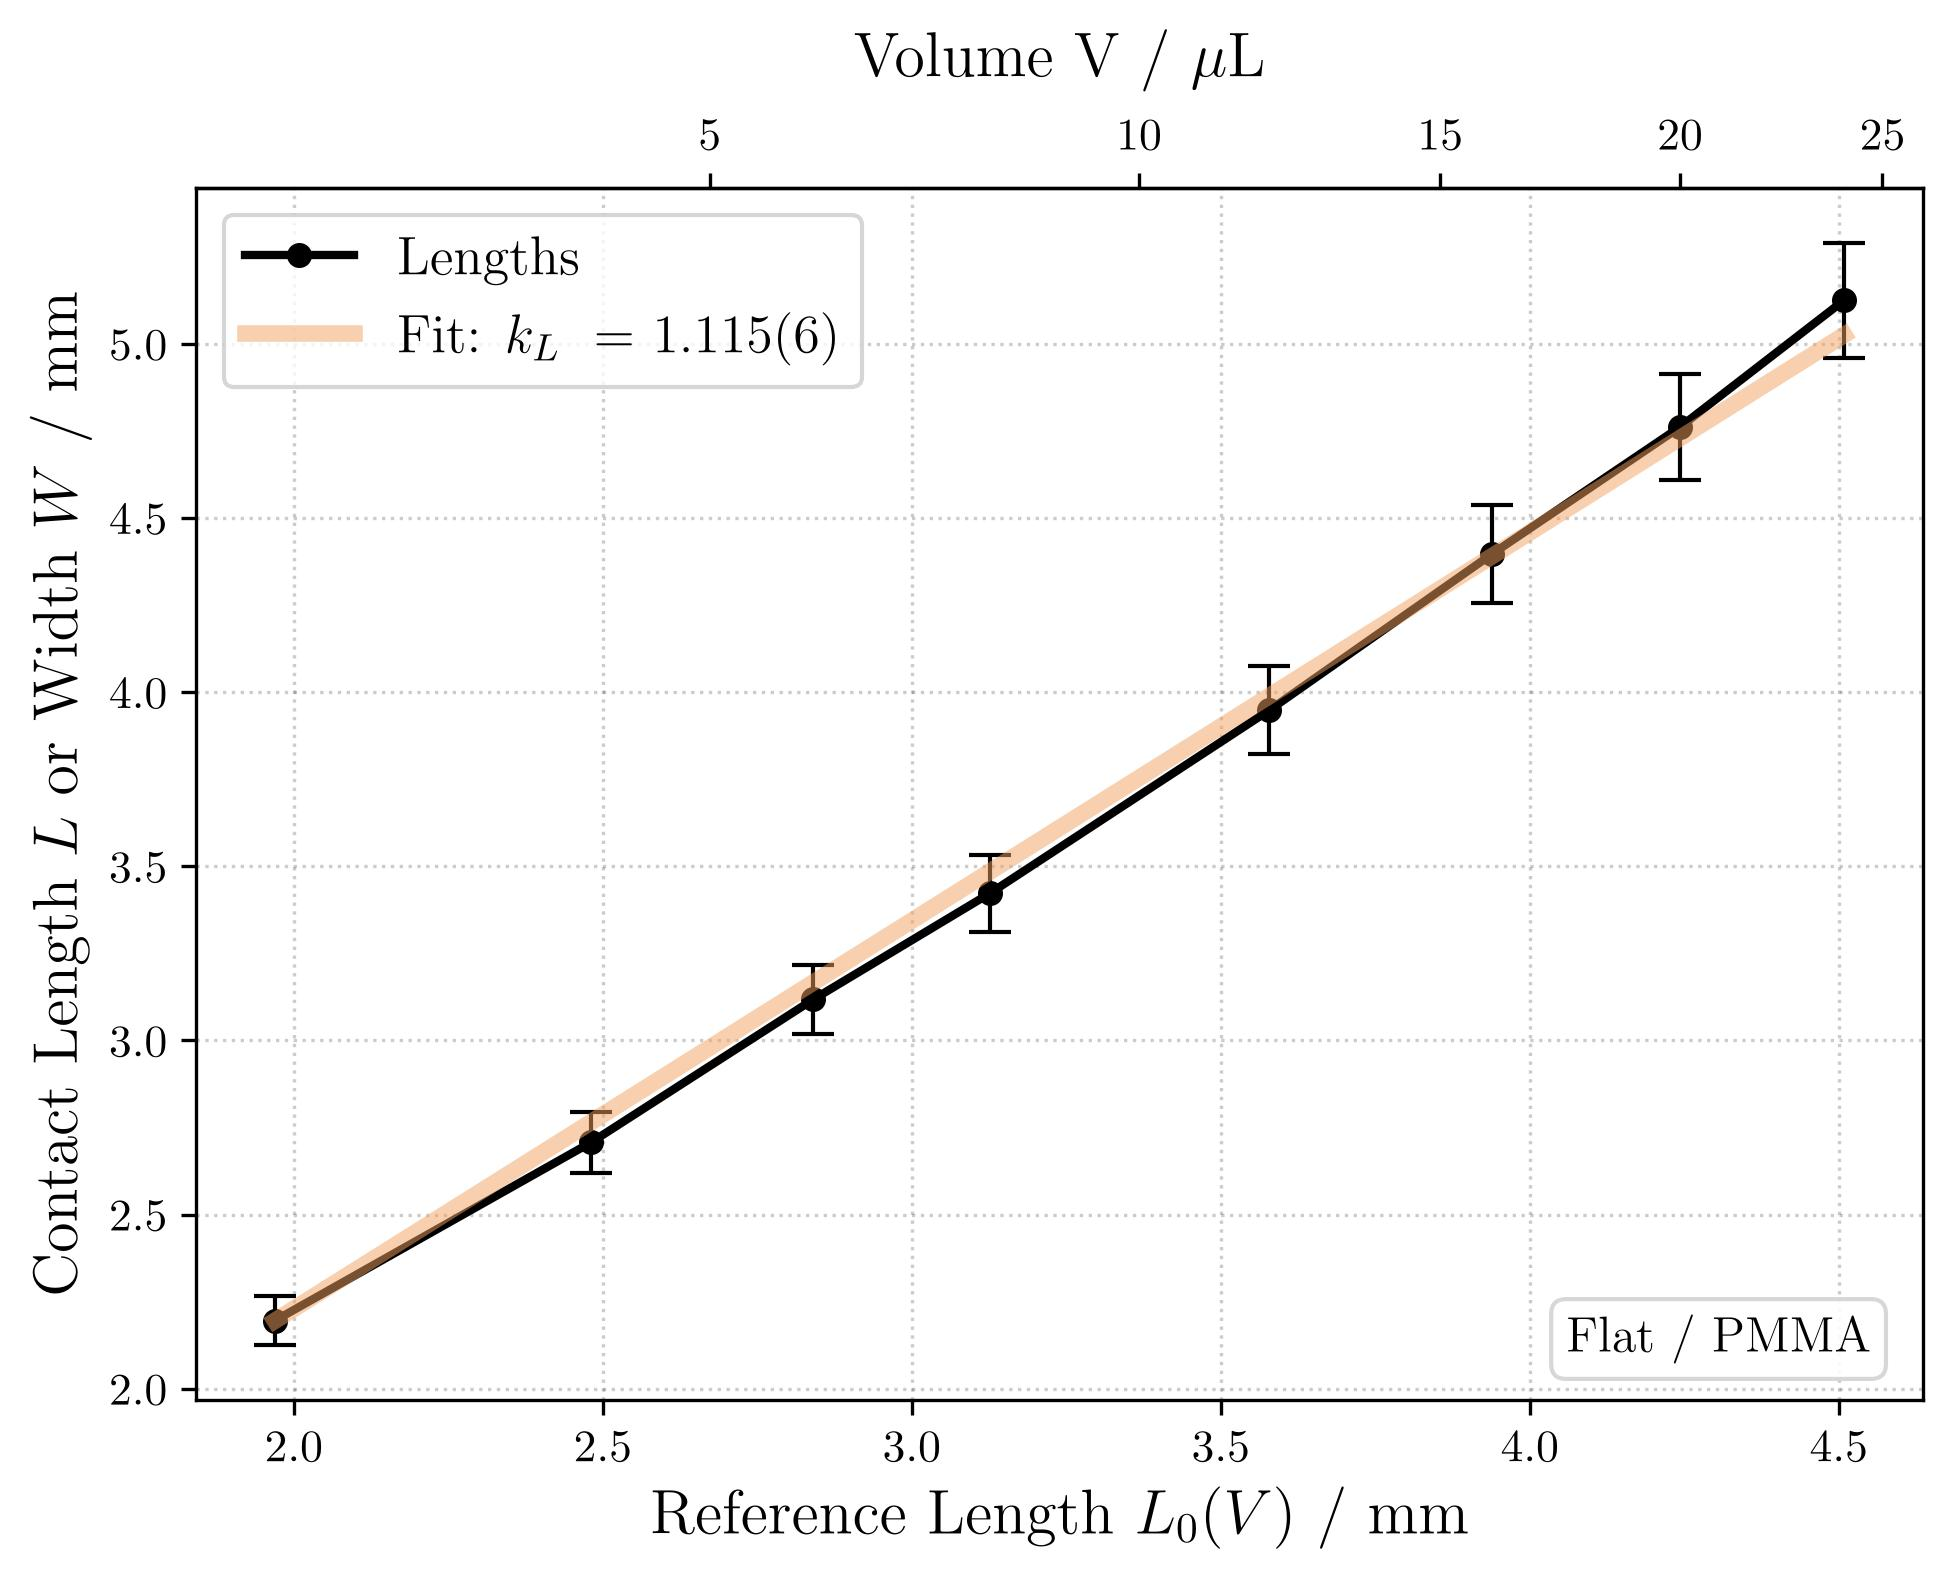
\includegraphics[width=0.55\linewidth]{../Plots/w06_flat_PMMA_L_fit.jpg}
        }
        \caption{Measurements of the contact length $L$ on a flat PMMA surface and its average (left). Contact length against the reference length $L_0(V)$ with linear fits according to \cref{eq:L_and_W_against_L0} (right). The model resembles the expectation closely as $k_L \approx 1$.}
        \label{fig:app:flat_data_fit_PMMA}
    \end{figure}


\newpage
\subsection{Measurements on PET}

    
% 4mm PET
    \begin{figure}[H]
        \centering
        \makebox[\textwidth]{        
        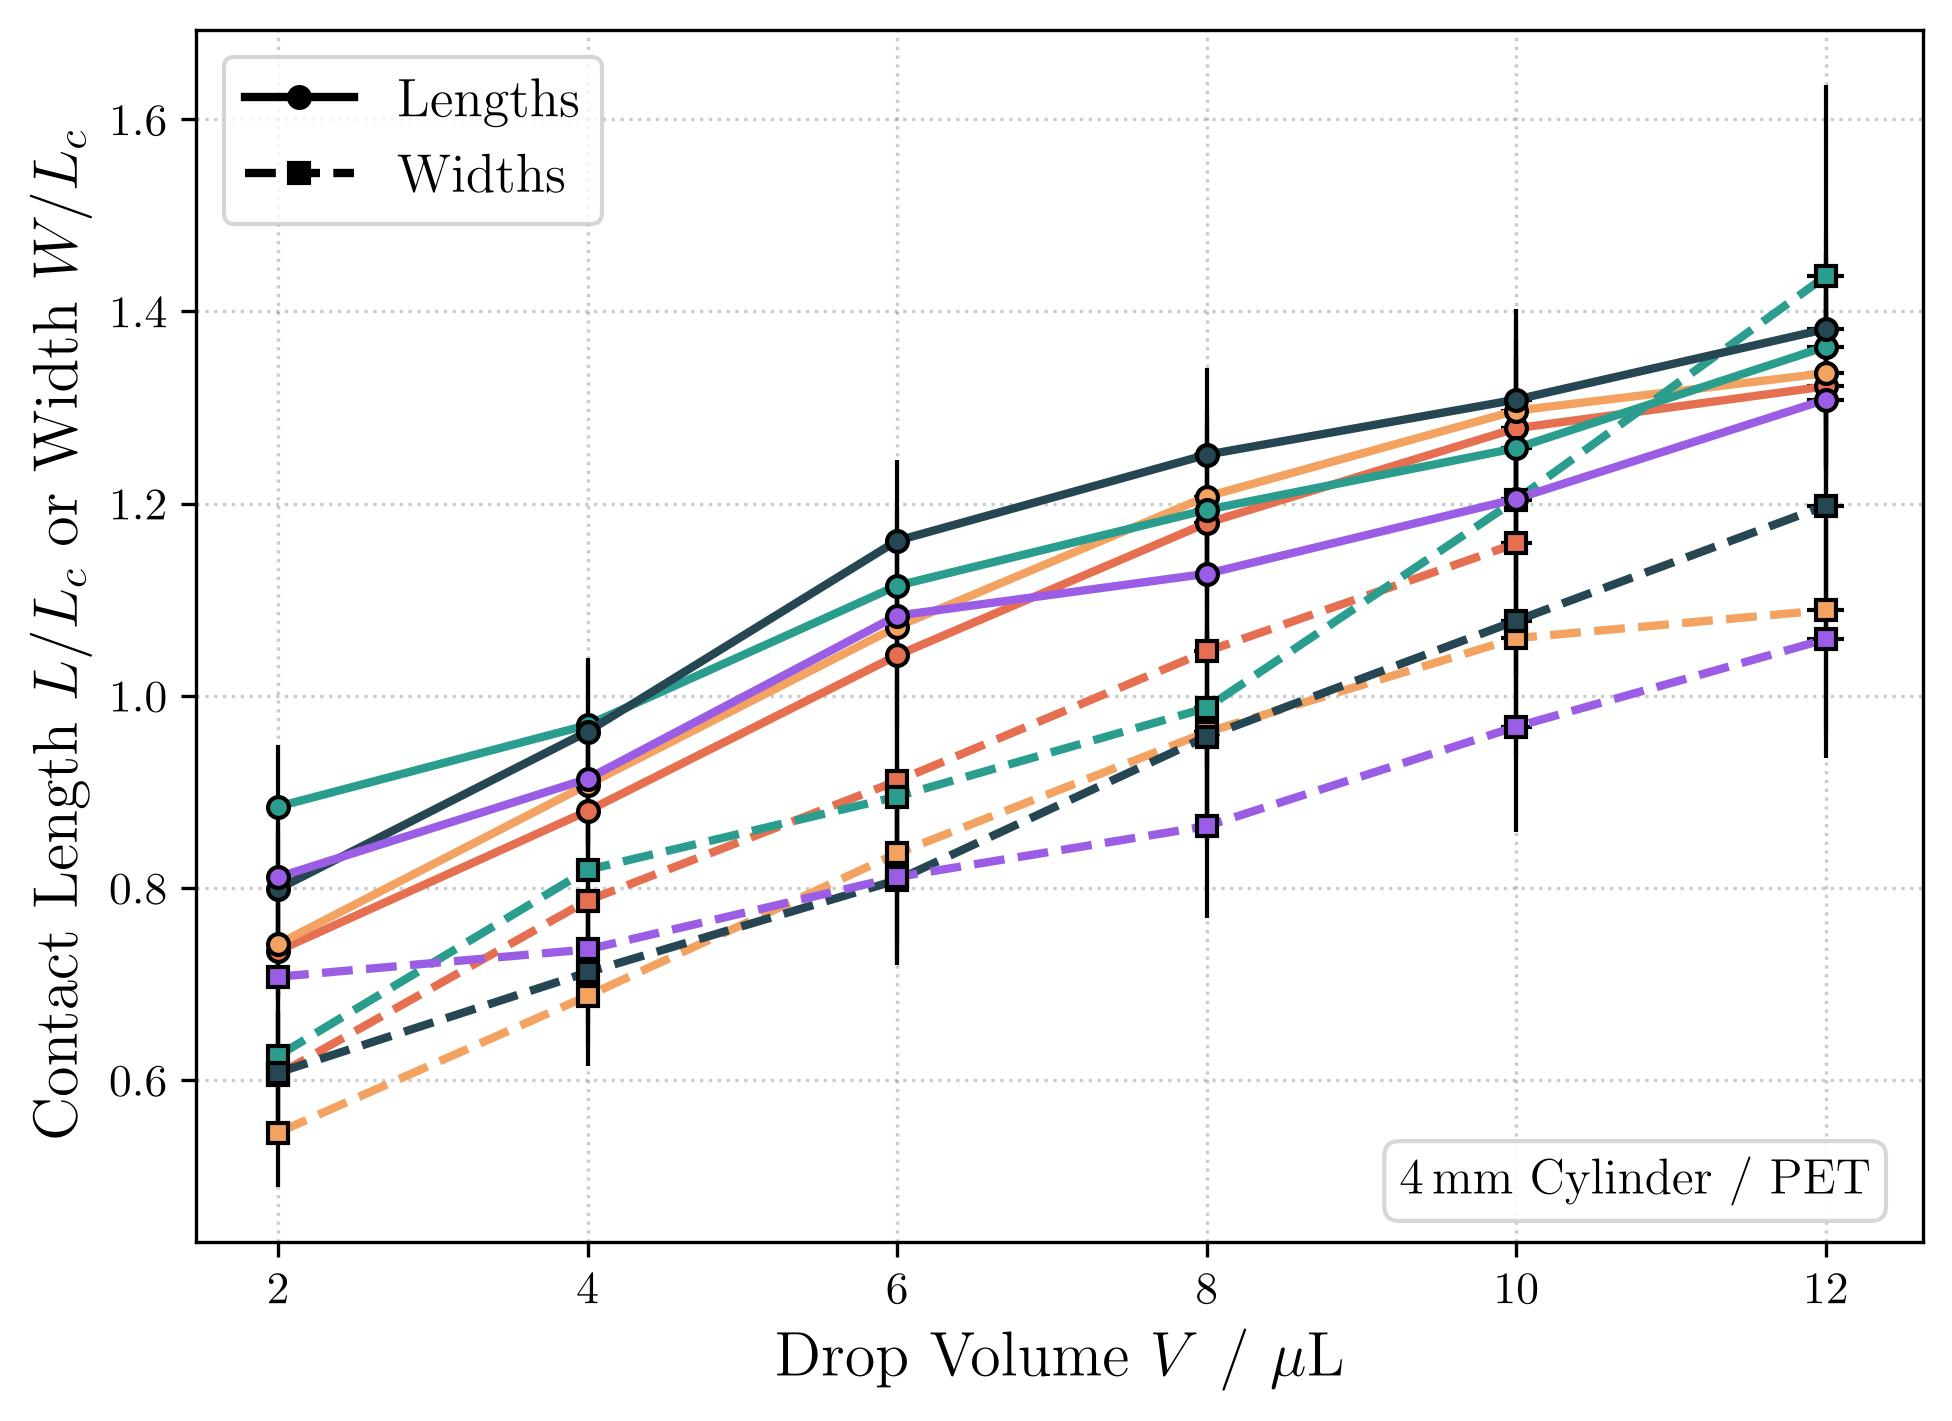
\includegraphics[width=0.55\linewidth]{../Plots/w06_04mm_PET_L+W.jpg}
        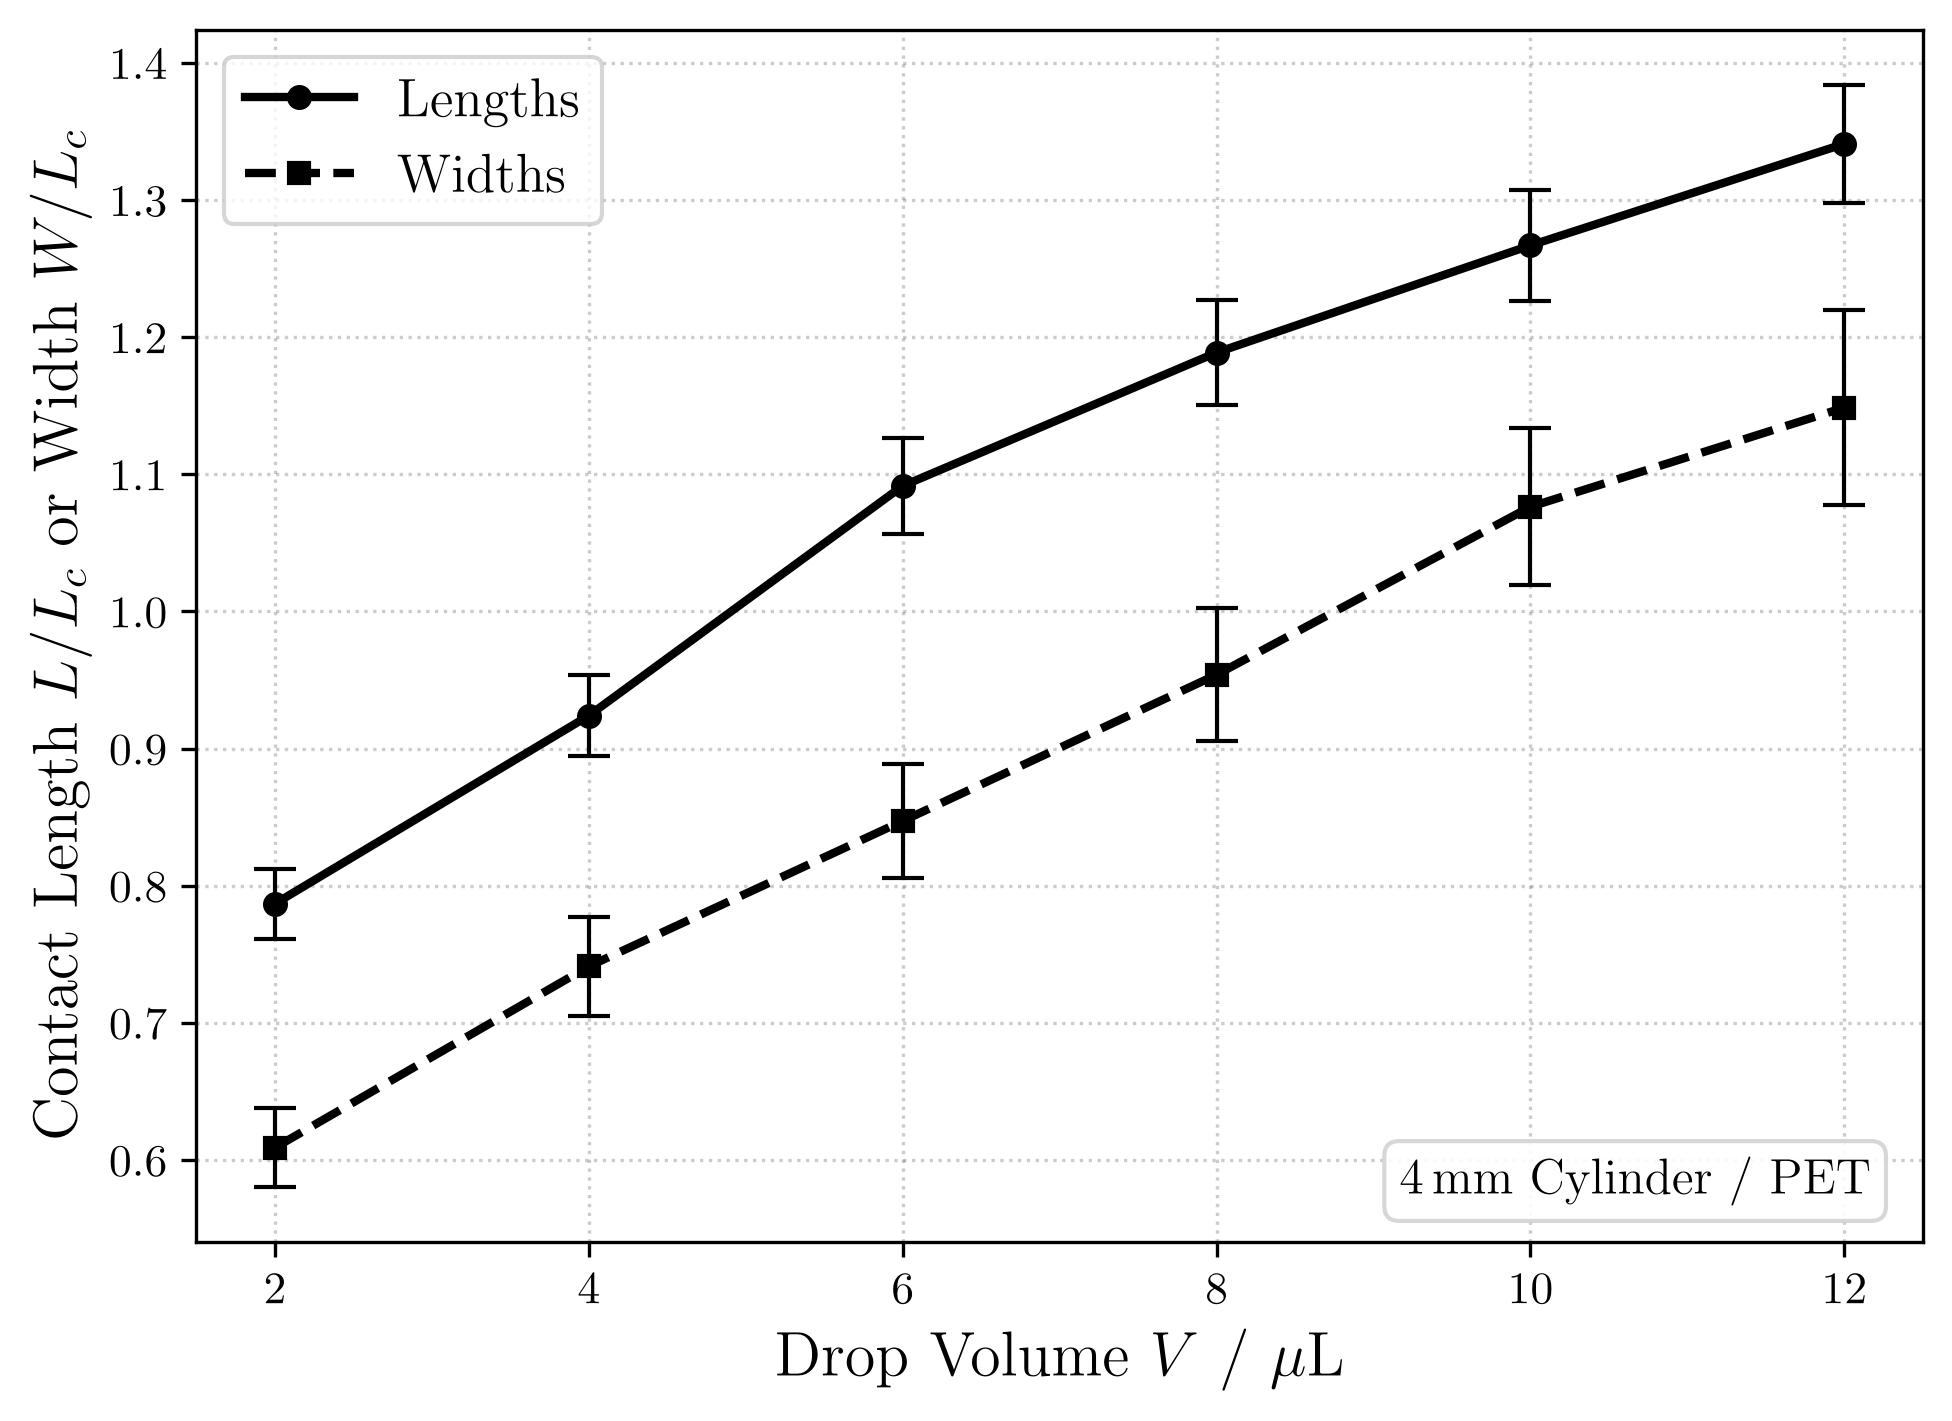
\includegraphics[width=0.55\linewidth]{../Plots/w06_04mm_PET_L+W_avg.jpg}
        }
        \caption{Measurements of contact length $L$ and width $W$ on the \SI{4}{\milli\meter} PET cylinder in raw (left) and averaged (right). Due to observed instability, the \SI{12}{\micro\liter} data points are not used in the analysis. $L$ and $W$ seem to converge, as gravity starts dominating over the surface tension for $L/L_c > 1$.}
        \label{fig:app:4mm_data_PET}
    \end{figure}

    \begin{figure}[H]
        \centering
        \makebox[\textwidth]{
        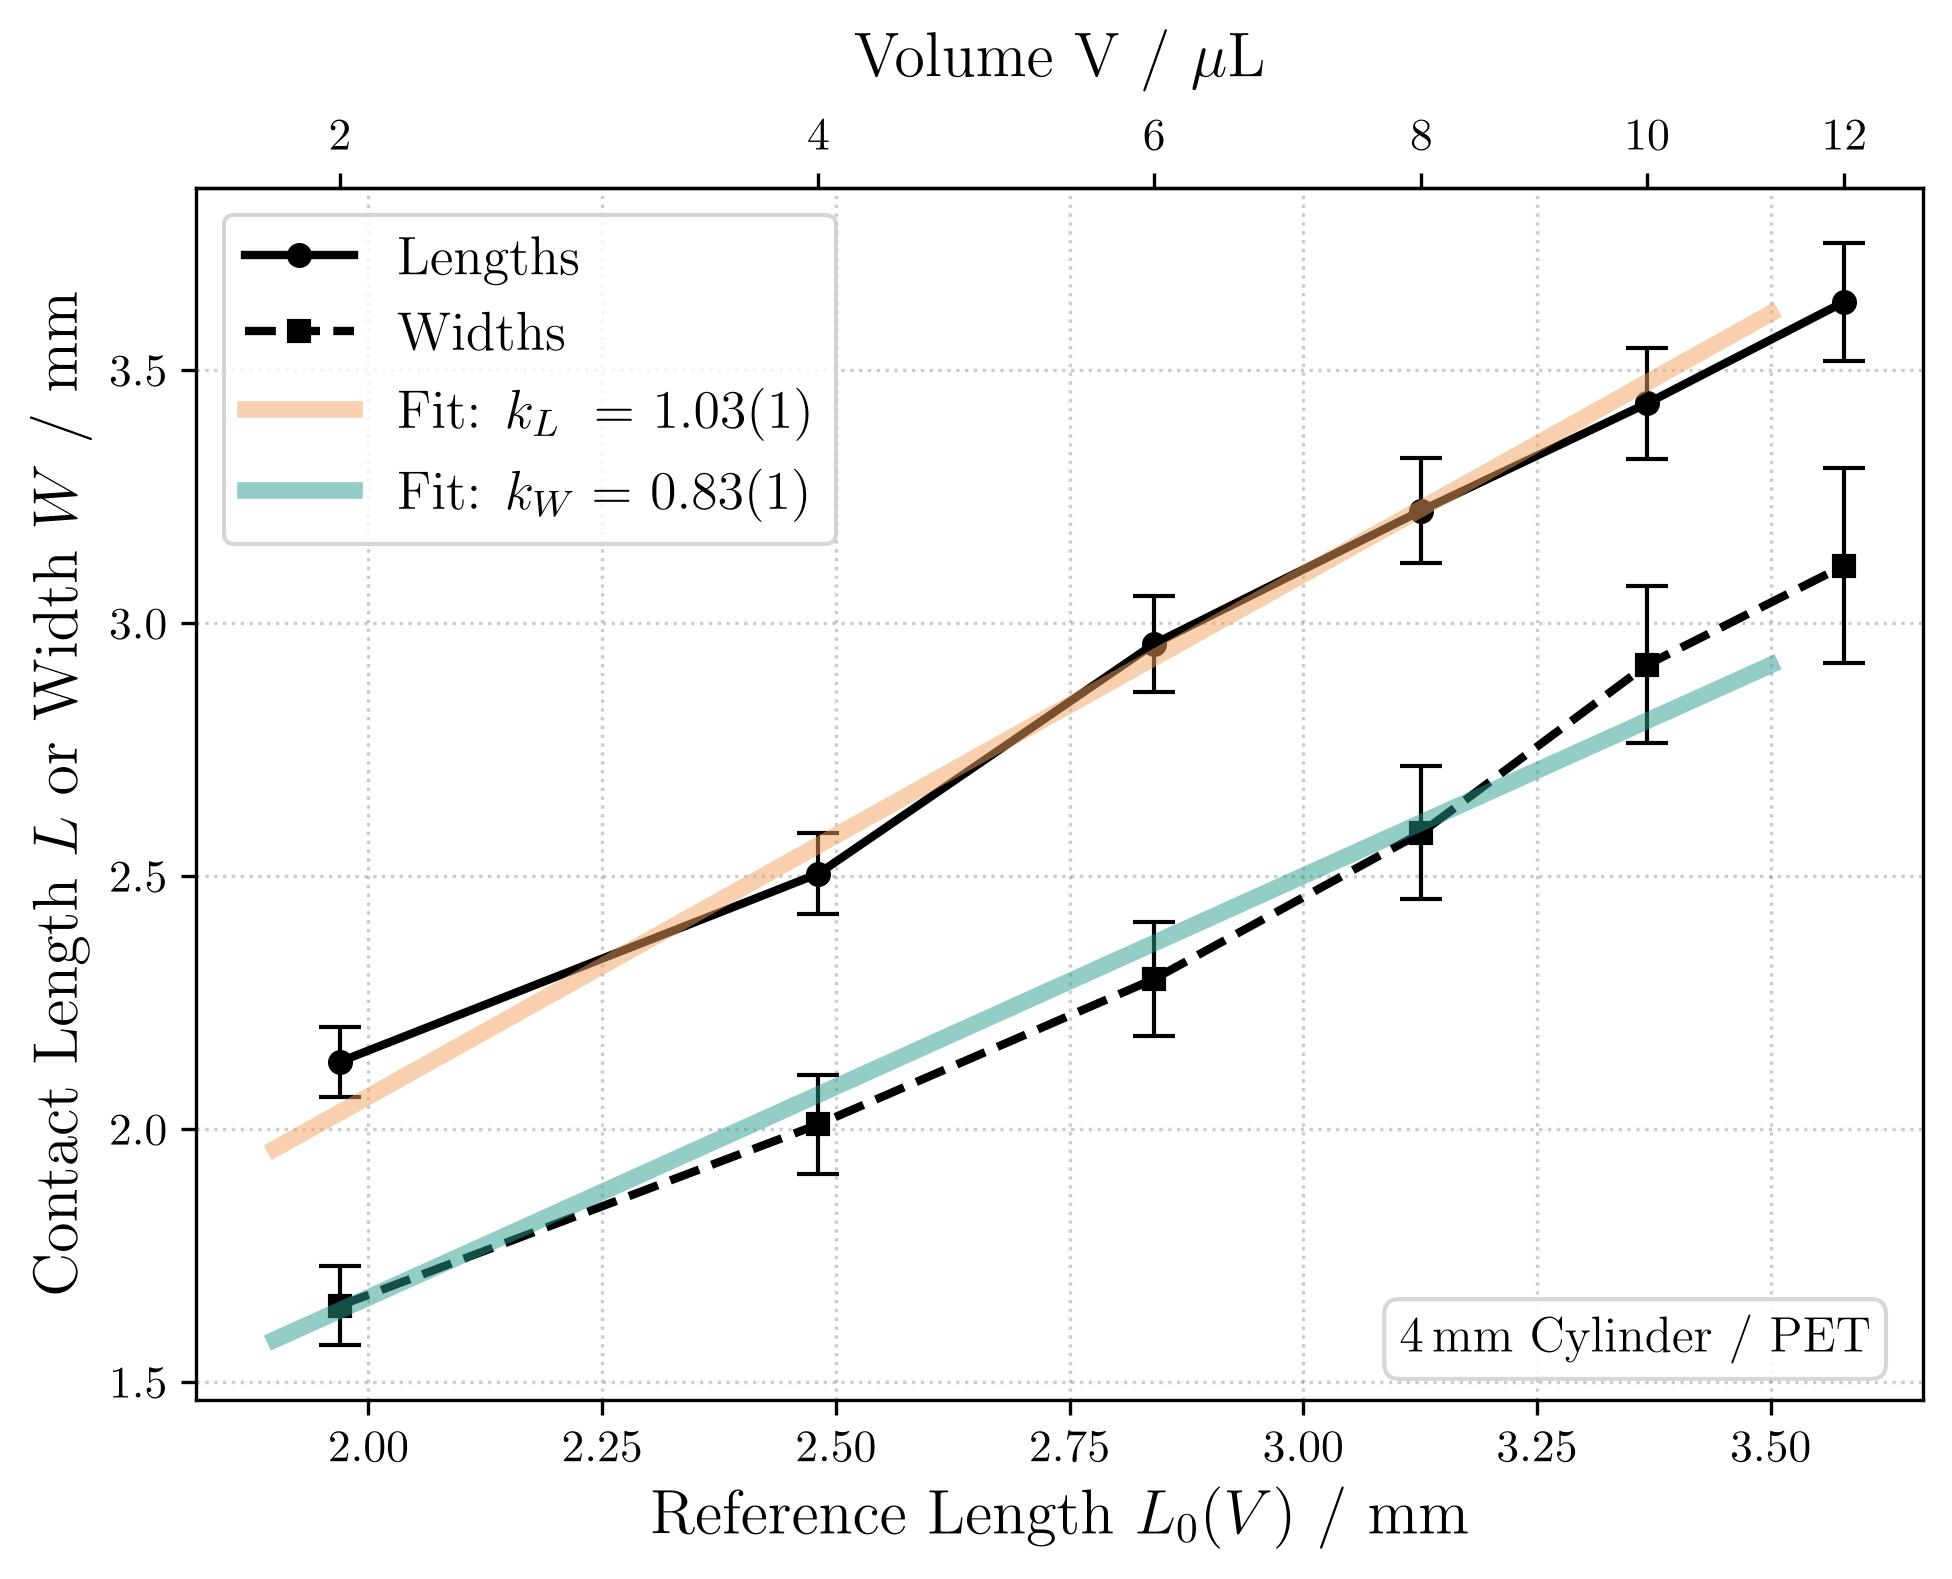
\includegraphics[width=0.55\linewidth]{../Plots/w06_04mm_PET_L+W_fit.jpg}
        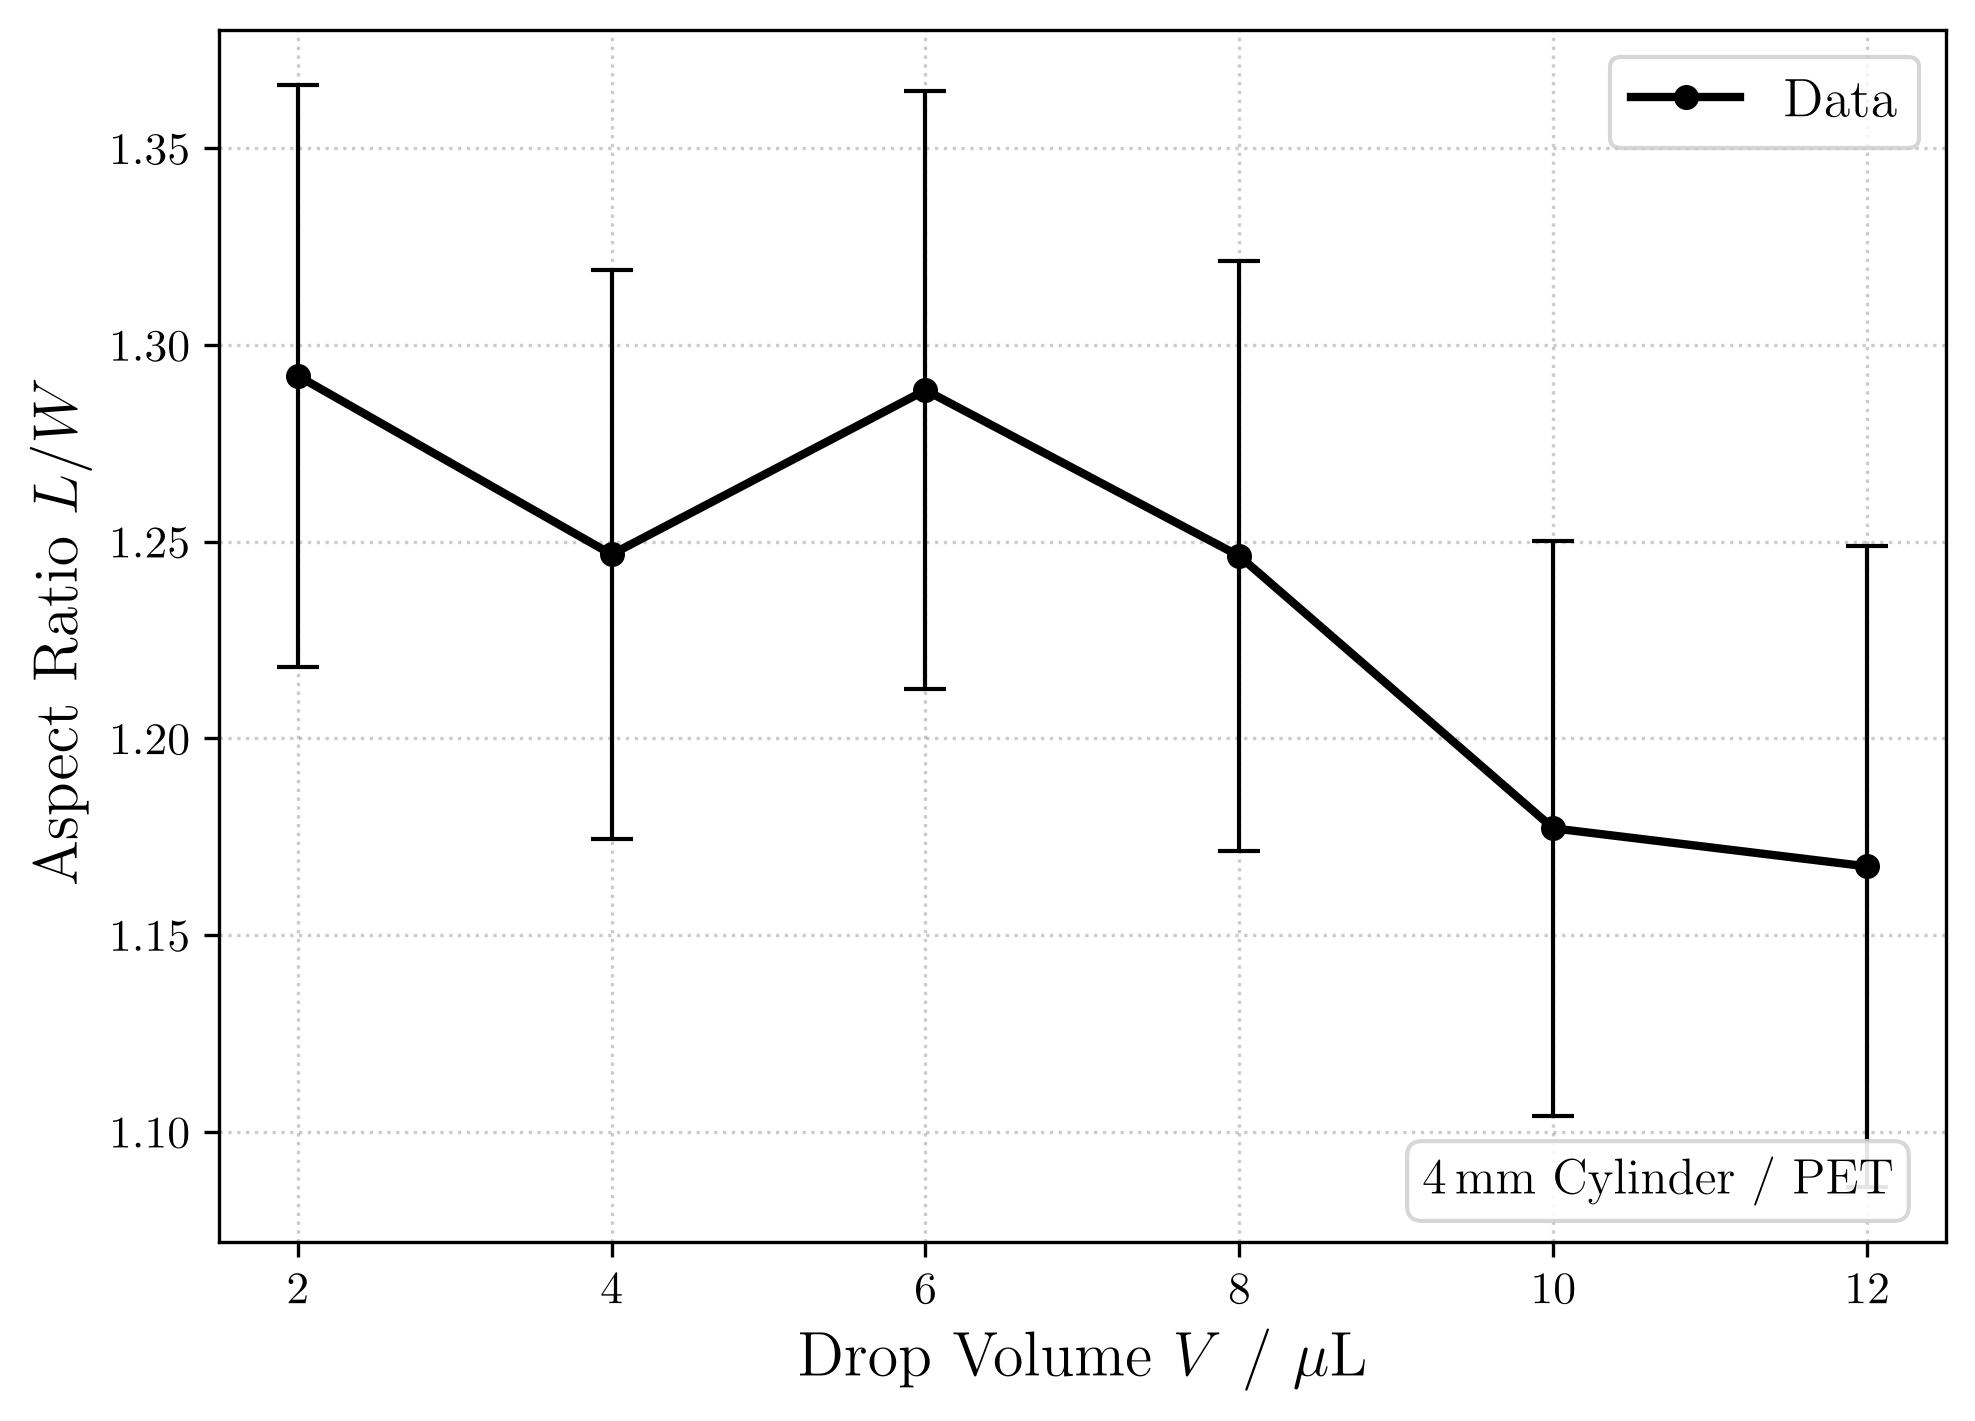
\includegraphics[width=0.55\linewidth]{../Plots/w06_04mm_PET_ratio.jpg}
        }
        \caption{Contact length and width against the reference length $L_0(V)$ with linear fits according to \cref{eq:L_and_W_against_L0} on the left. Again, the linear model is confirmed with high flexibility $(\chi^2 \ll 1)$ and $L > W$ for all $V$. Their aspect ratios $L/W$ (right) on the \SI{4}{\milli\meter} PET cylinder trends visibly down to $1$, where the droplet width will exceed its length.}
        \label{fig:app:4mm_fit_ratio_PET}
    \end{figure}



    
% 10mm PET
    \begin{figure}[H]
        \centering
        \makebox[\textwidth]{
        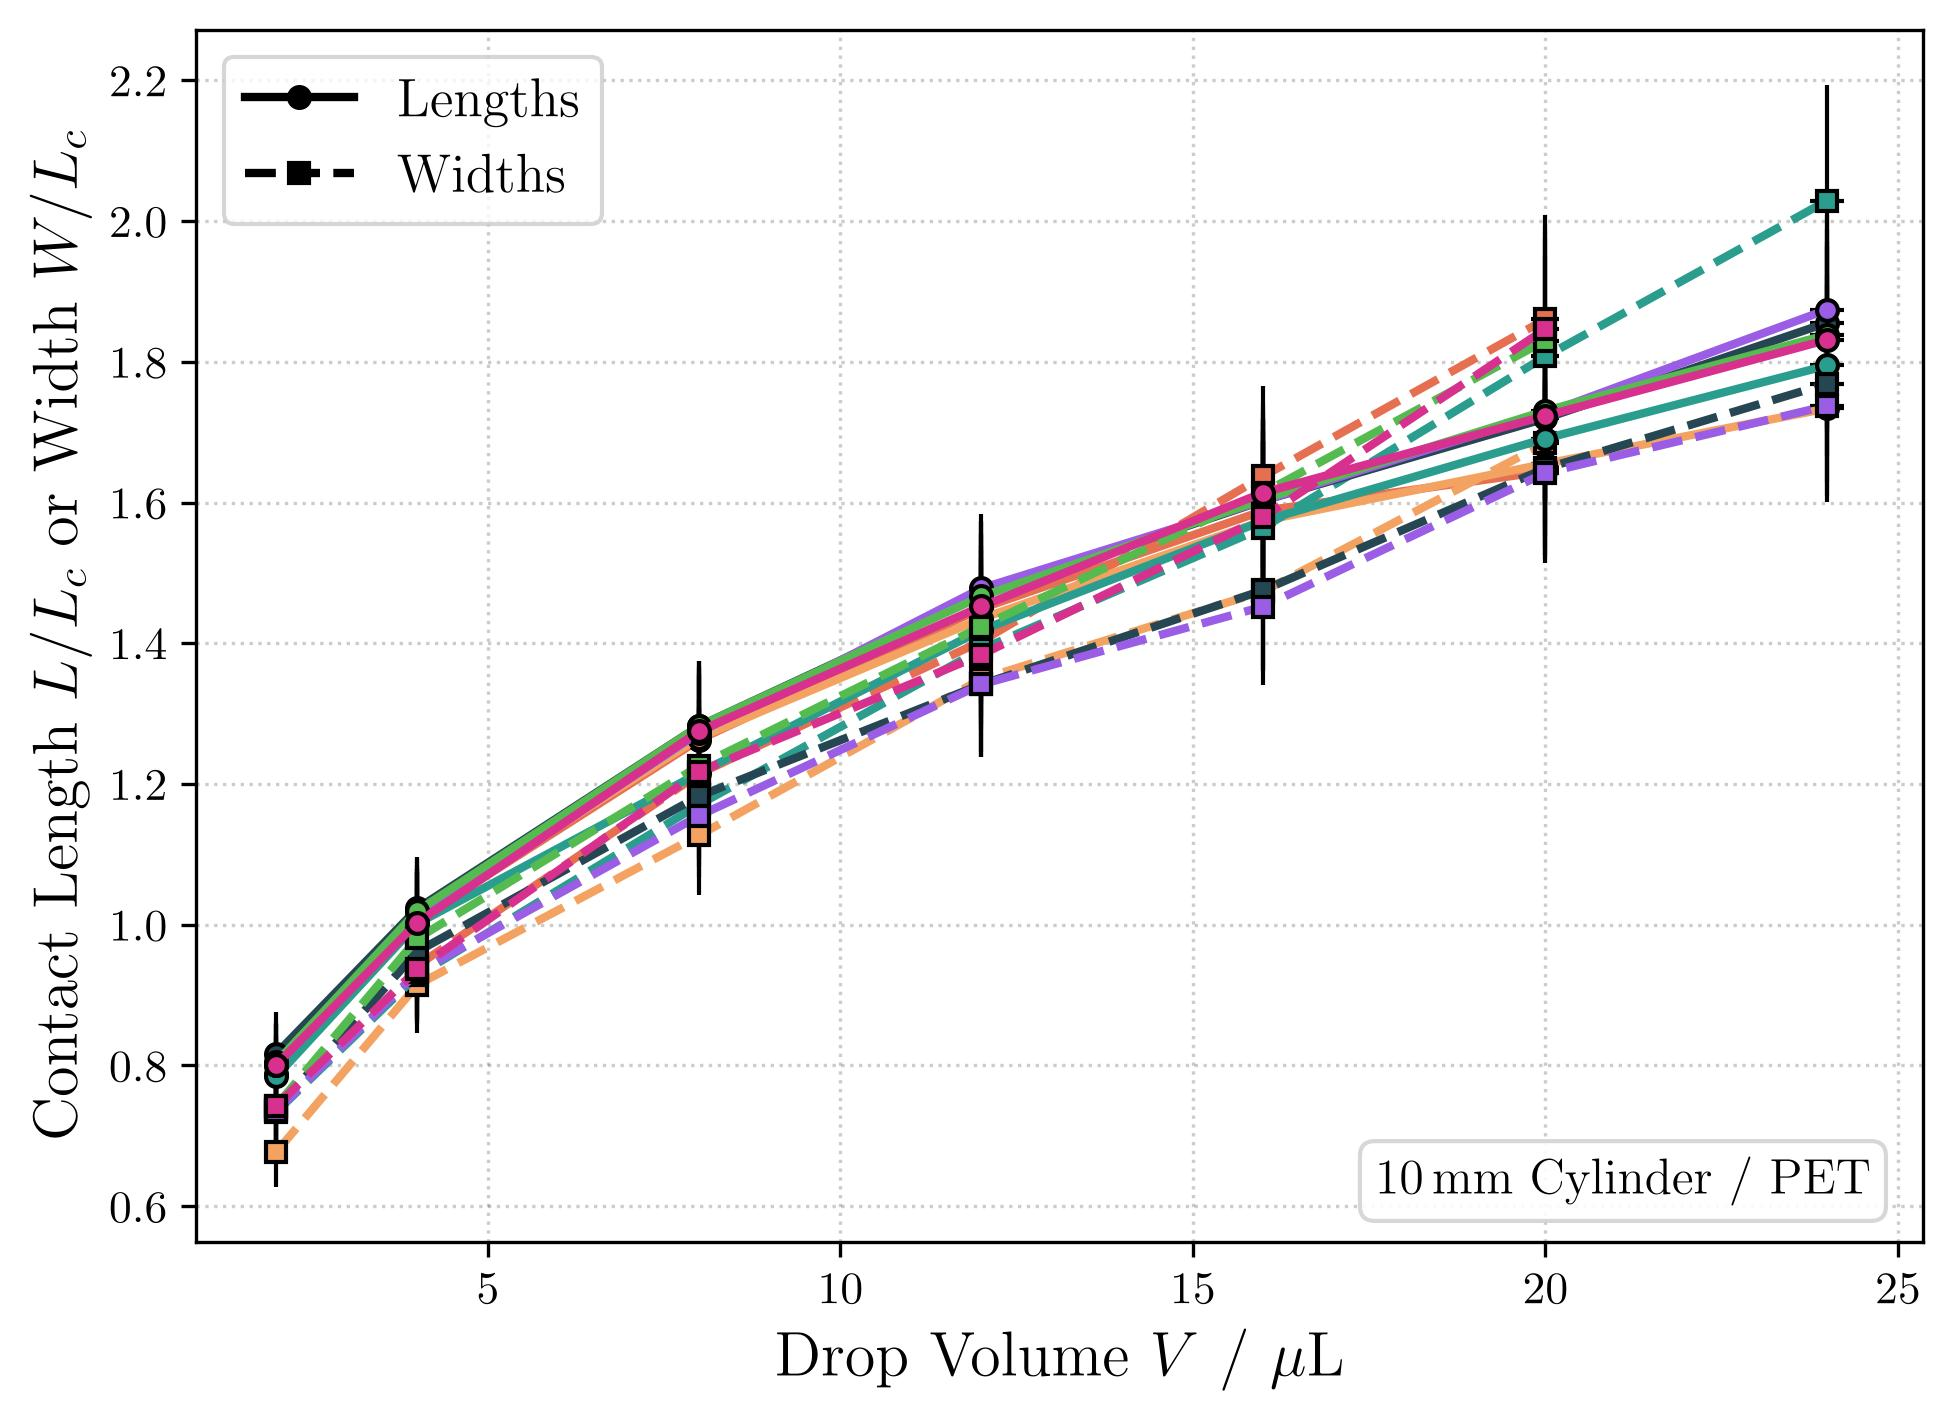
\includegraphics[width=0.55\linewidth]{../Plots/w06_10mm_PET_L+W.jpg}
        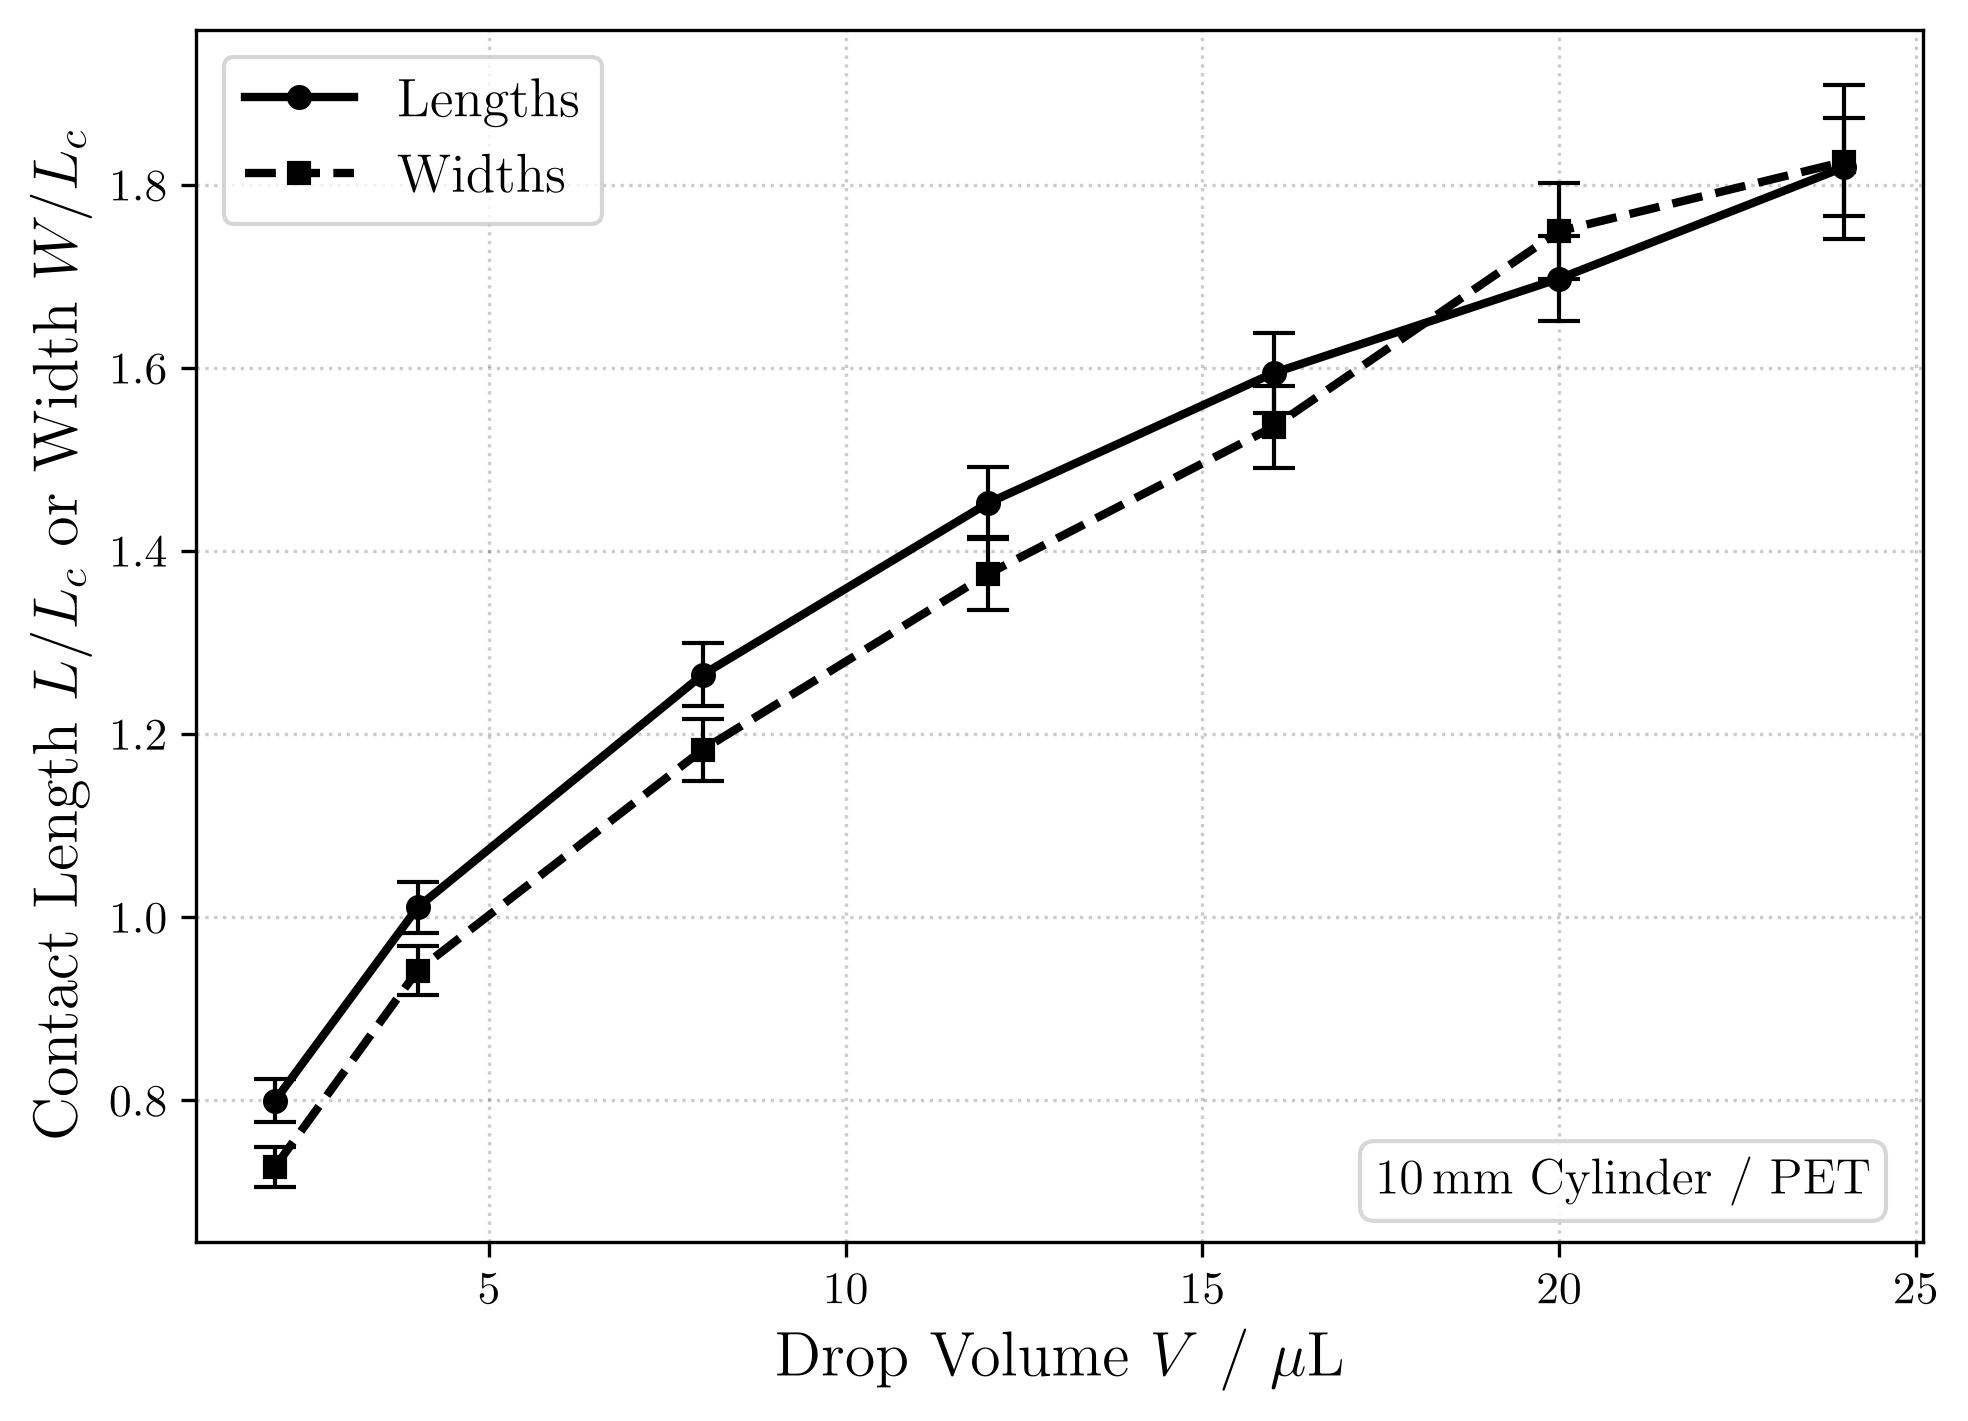
\includegraphics[width=0.55\linewidth]{../Plots/w06_10mm_PET_L+W_avg.jpg}
        }
        \caption{Measurements of contact length $L$ and width $W$ on the \SI{10}{\milli\meter} PET cylinder in raw (left) and averaged (right). The length $L$ is overtaking by the width $W$ at \SI{18}{\micro\liter}, indicating the domination of gravity over surface tension $(L/L_c > 1.6)$. Due to observed instability, the \SI{20}{\micro\liter} \& \SI{24}{\micro\liter} data points are not used in the quantitative analysis.}
        \label{fig:app:10mm_data_PET}
    \end{figure}

    \begin{figure}[H]
        \centering
        \makebox[\textwidth]{
        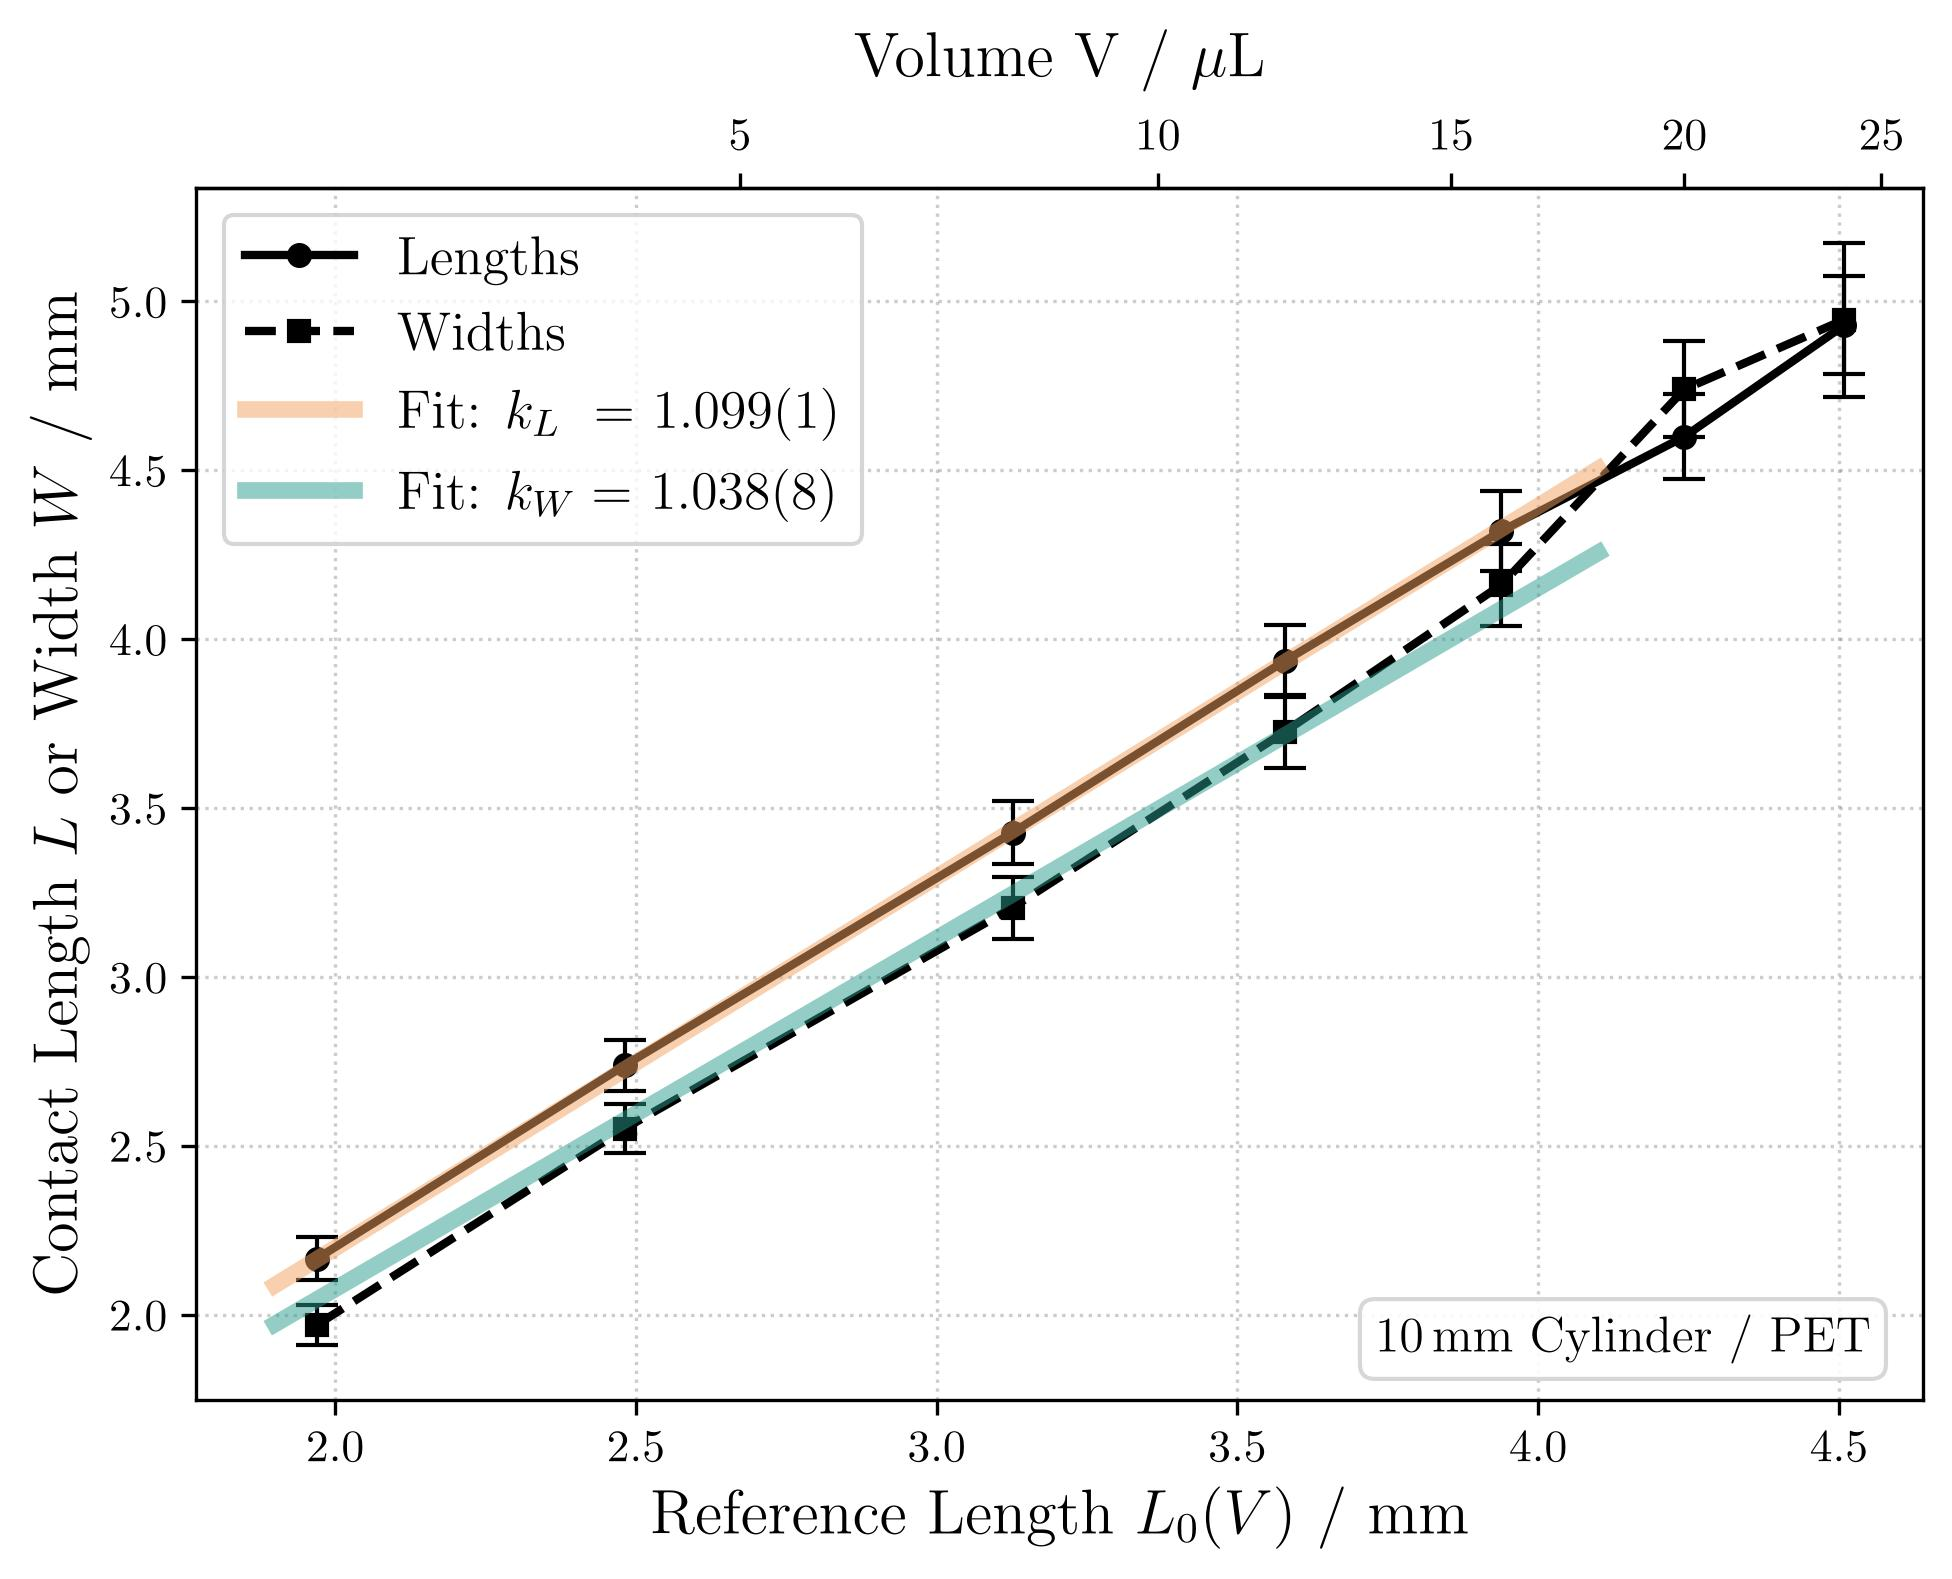
\includegraphics[width=0.55\linewidth]{../Plots/w06_10mm_PET_L+W_fit.jpg}
        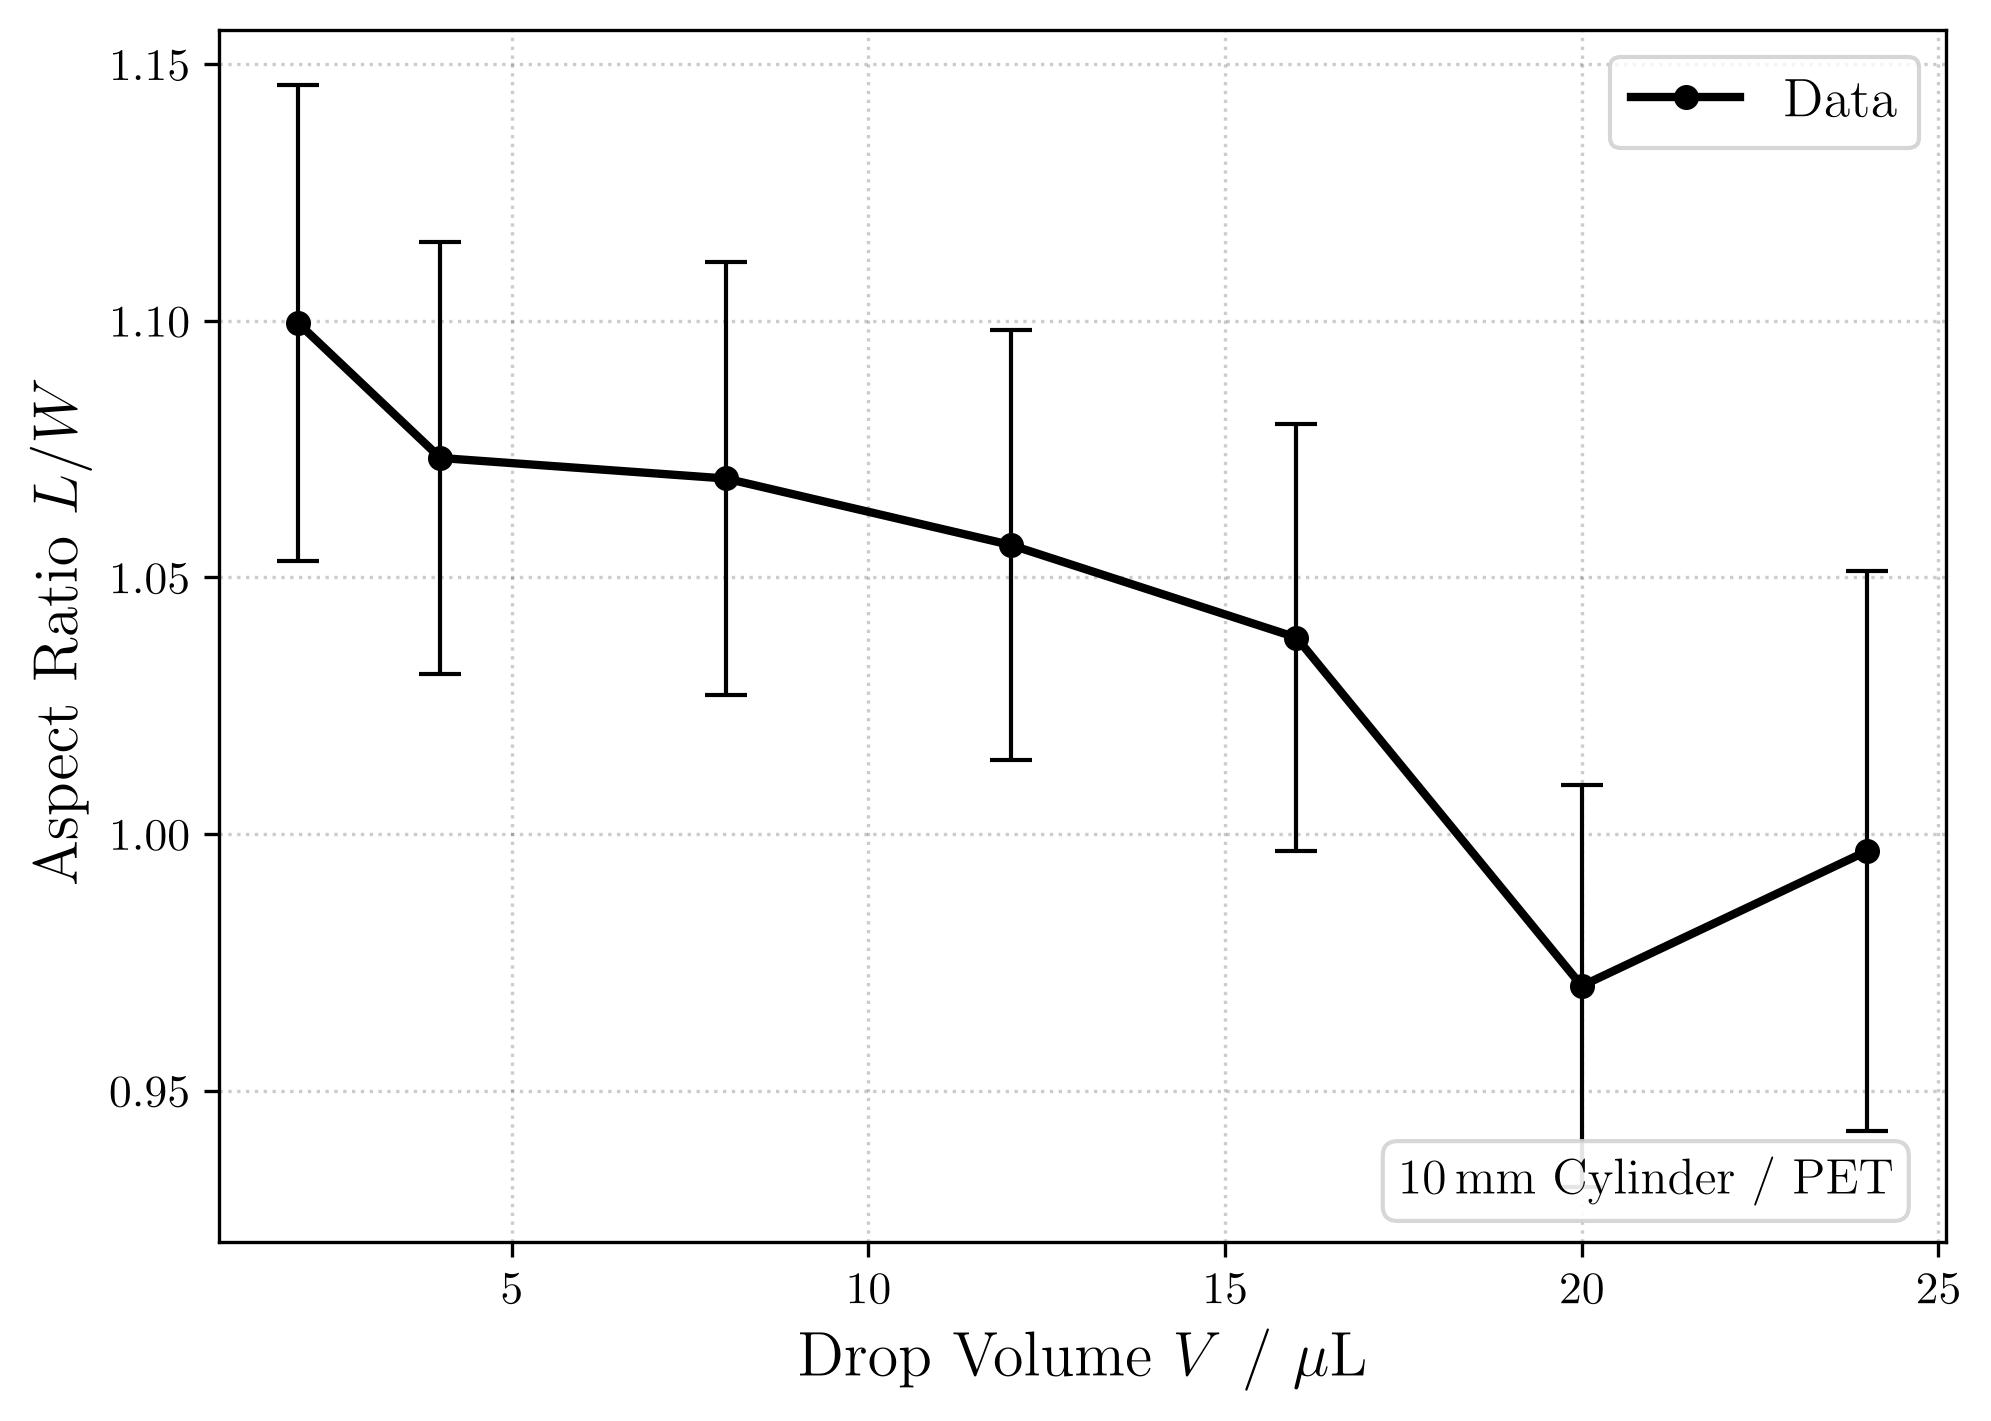
\includegraphics[width=0.55\linewidth]{../Plots/w06_10mm_PET_ratio.jpg}
        }
        \caption{Contact length and width against the reference length $L_0(V)$ with linear fits according to \cref{eq:L_and_W_against_L0} on the left. As before, the linear model is confirmed with high flexibility $(\chi^2 \ll 1)$ and $k_L$ , $k_W > 1$ indicates the \enquote{rounded} drop geometry. Their aspect ratios $L/W$ (right) on the \SI{10}{\milli\meter} PET cylinder confirm the overtaking of gravity through the decrease in $L/W$ down to below $1.0$.  }
        \label{fig:app:10mm_fit_ratio_PET}
    \end{figure}


% flat PET
    \begin{figure}[H]
        \centering
        \makebox[\textwidth]{
        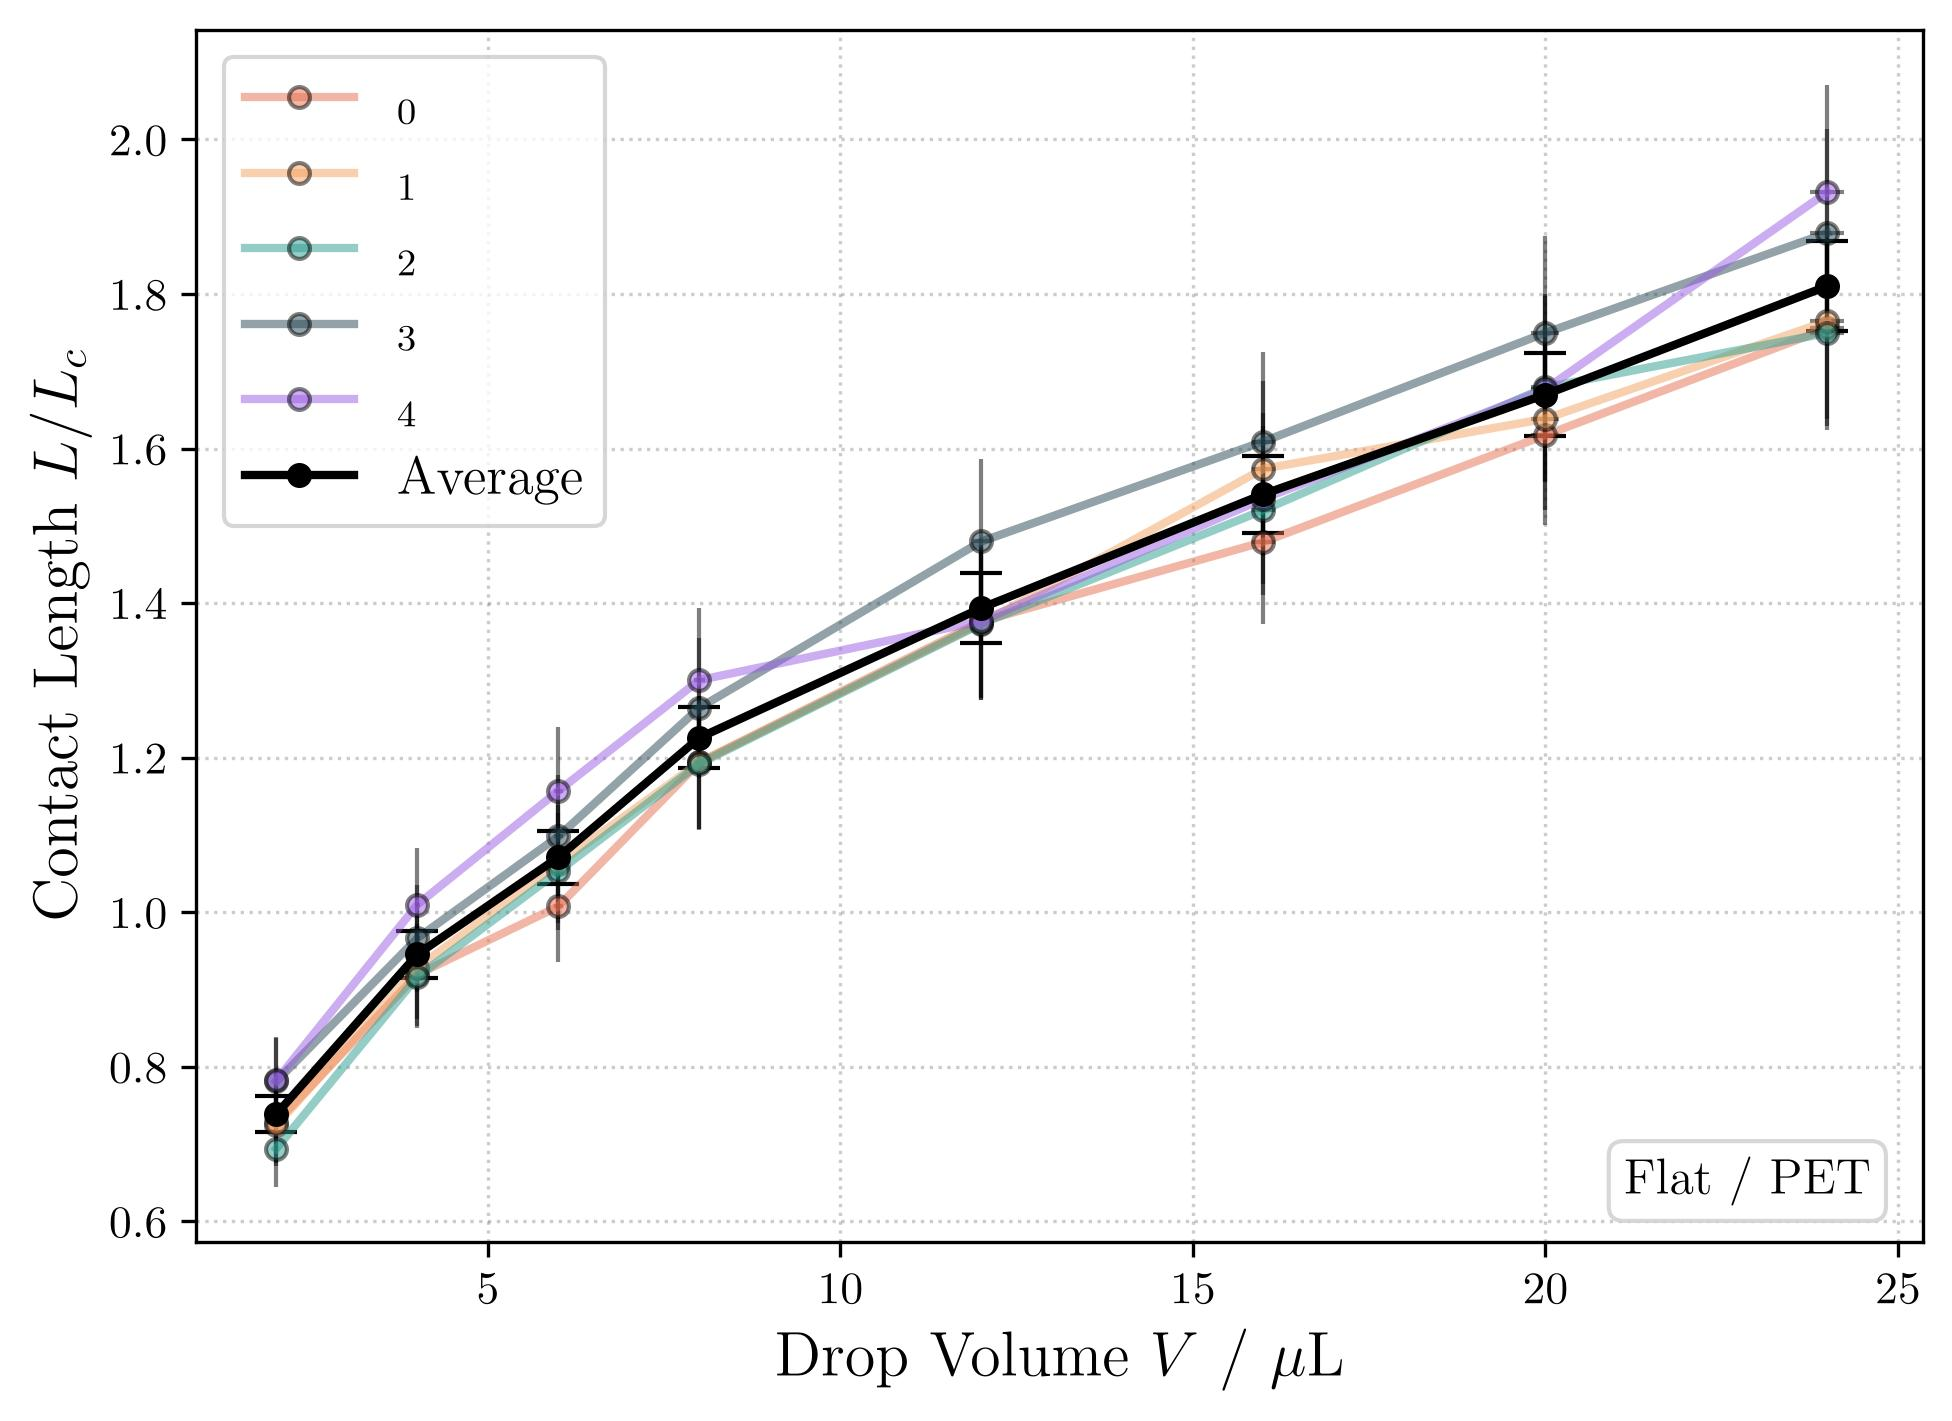
\includegraphics[width=0.55\linewidth]{../Plots/w06_flat_PET_L.jpg}
        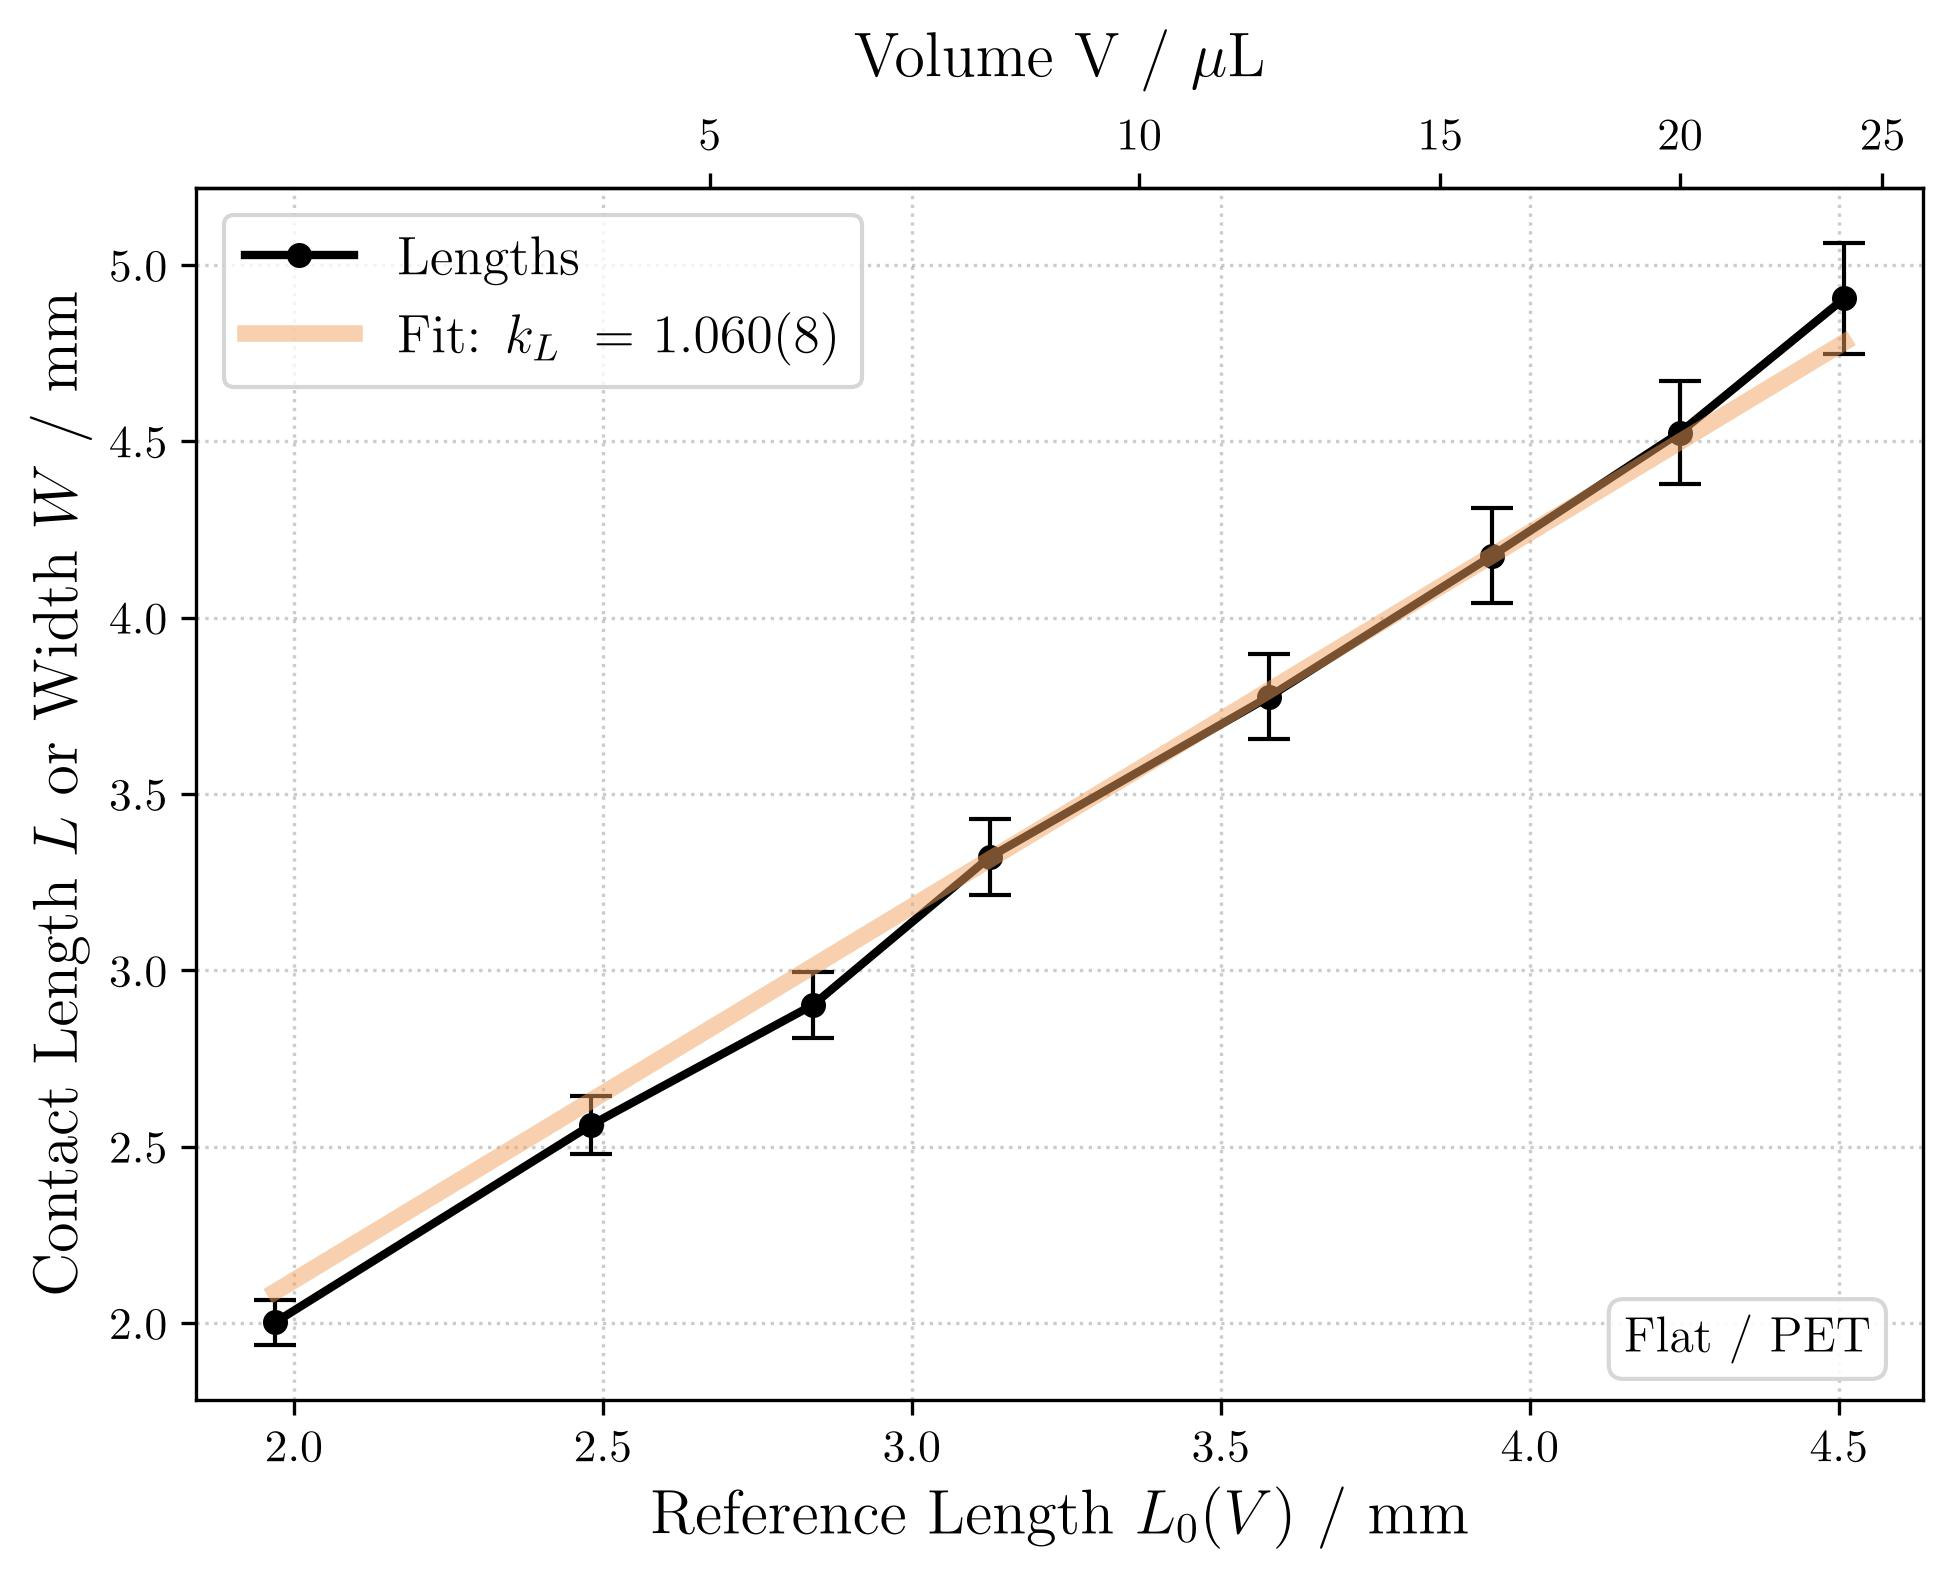
\includegraphics[width=0.55\linewidth]{../Plots/w06_flat_PET_L_fit.jpg}
        }
        \caption{Measurements of the contact length $L$ on a flat PET surface and its average (left). Contact length against the reference length $L_0(V)$ with linear fits according to \cref{eq:L_and_W_against_L0} (right). The model resembles the expectation closely as $k_L \approx 1$.}
        \label{fig:app:flat_data_fit_PET}
    \end{figure}

    \newpage


\subsection{Measurement Collages on PMMA}
    \label{app:collages_PMMA}

    \begin{figure}[H]
        \centering
        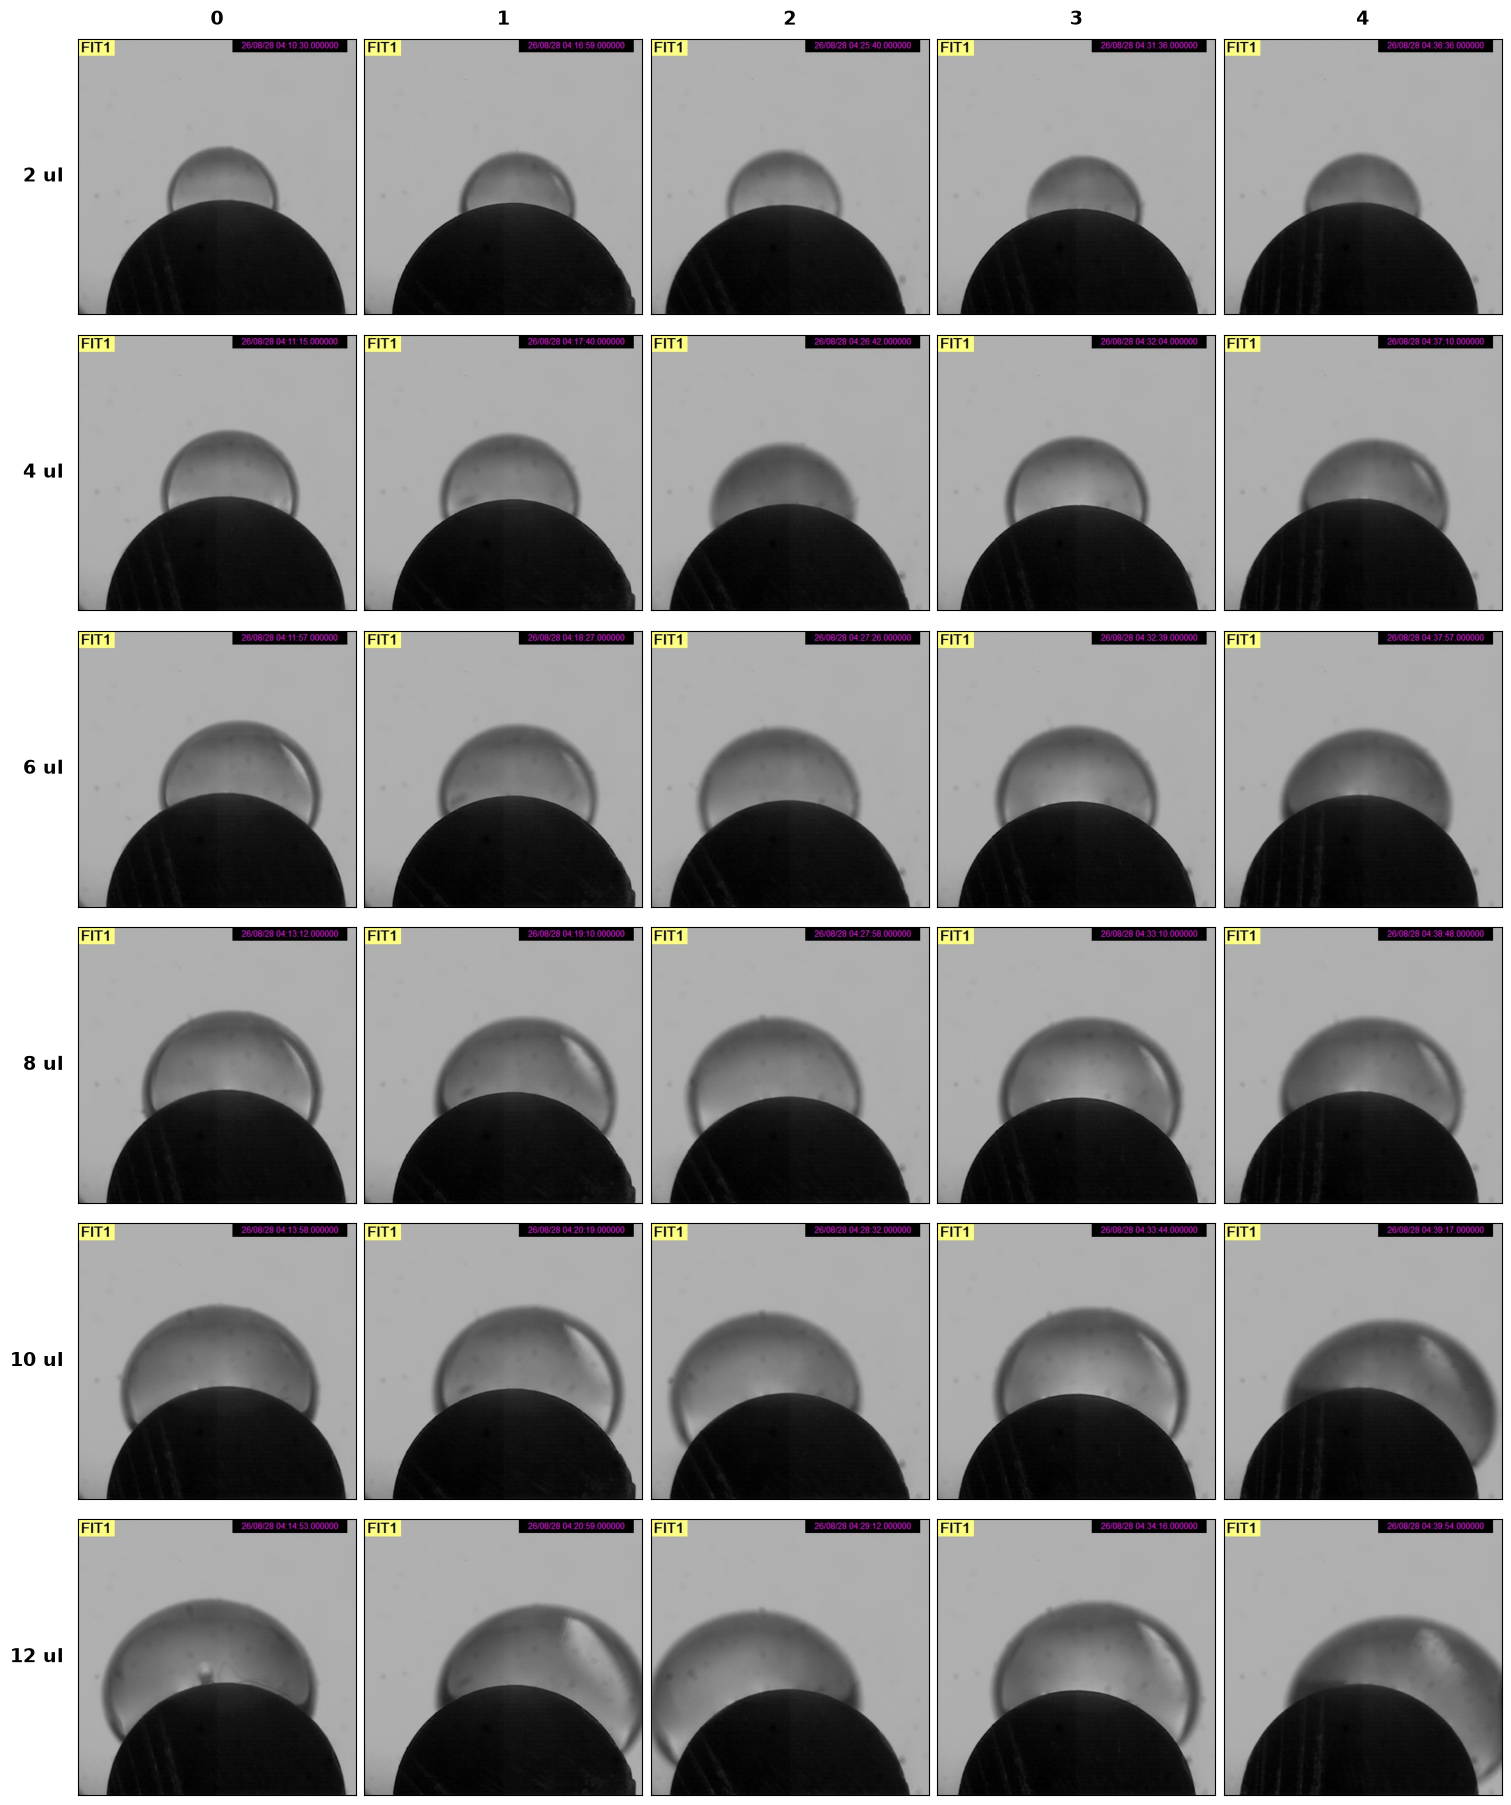
\includegraphics[width=\linewidth]{../Collages/collage_PMMA_2-12ul_4mm_front.png}
        \caption{Measurements on the \SI{4}{\milli\meter} PMMA cylinder from the front perspective.}
    \end{figure}

    \begin{figure}[H]
        \centering
        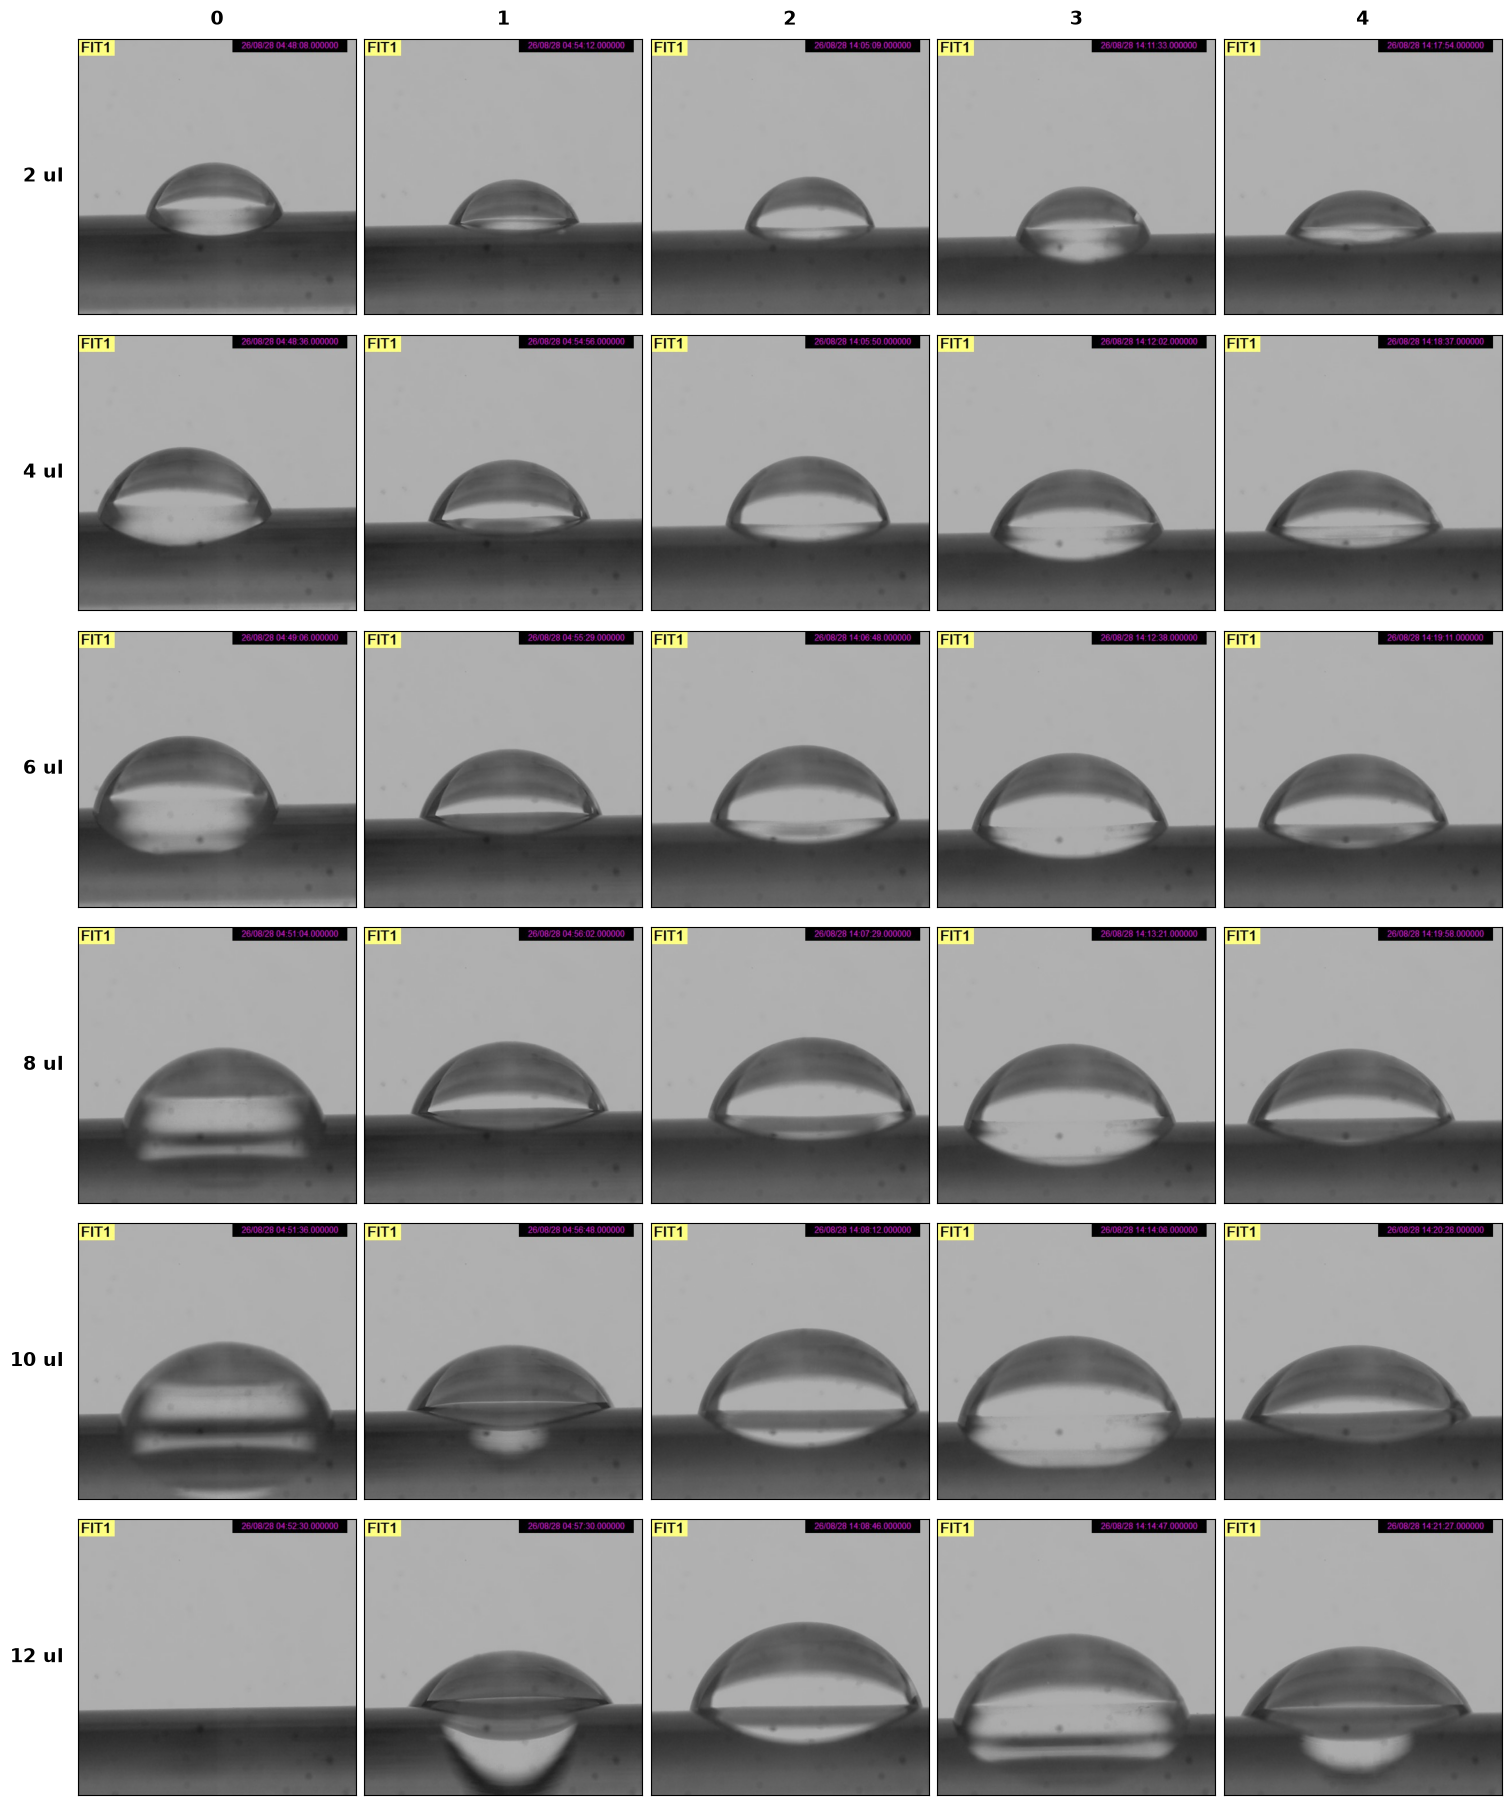
\includegraphics[width=\linewidth]{../Collages/collage_PMMA_2-12ul_4mm_side.png}
        \caption{Measurements on the \SI{4}{\milli\meter} PMMA cylinder from the side perspective.}
    \end{figure}

    \begin{figure}[H]
        \centering
        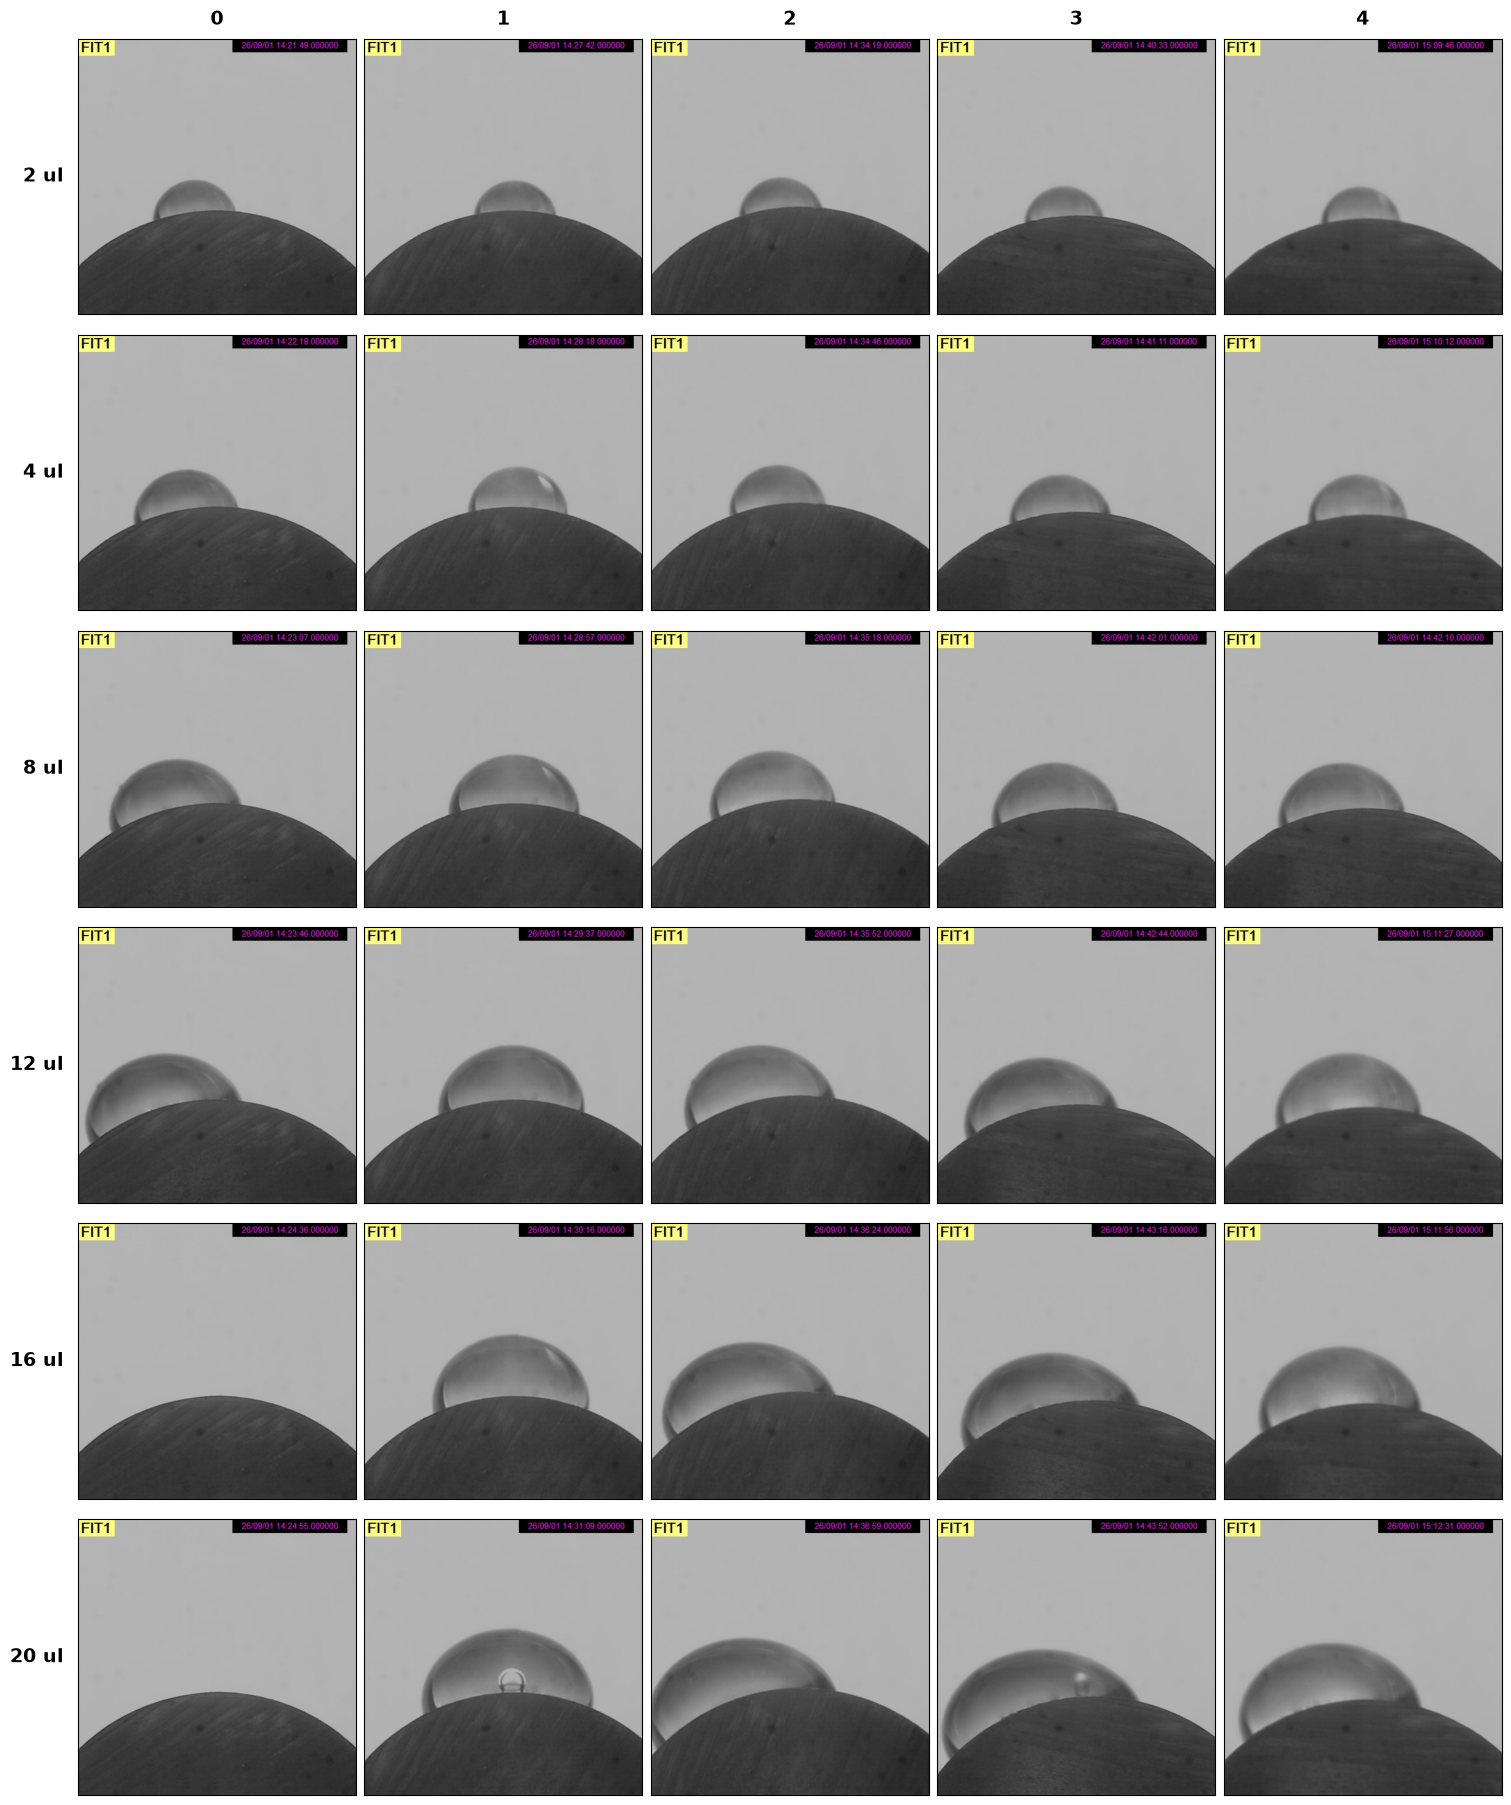
\includegraphics[width=\linewidth]{../Collages/collage_PMMA_2-30ul_10mm_front.png}
        \caption{Measurements on the \SI{10}{\milli\meter} PMMA cylinder from the front perspective.}
    \end{figure}

    \begin{figure}[H]
        \centering
        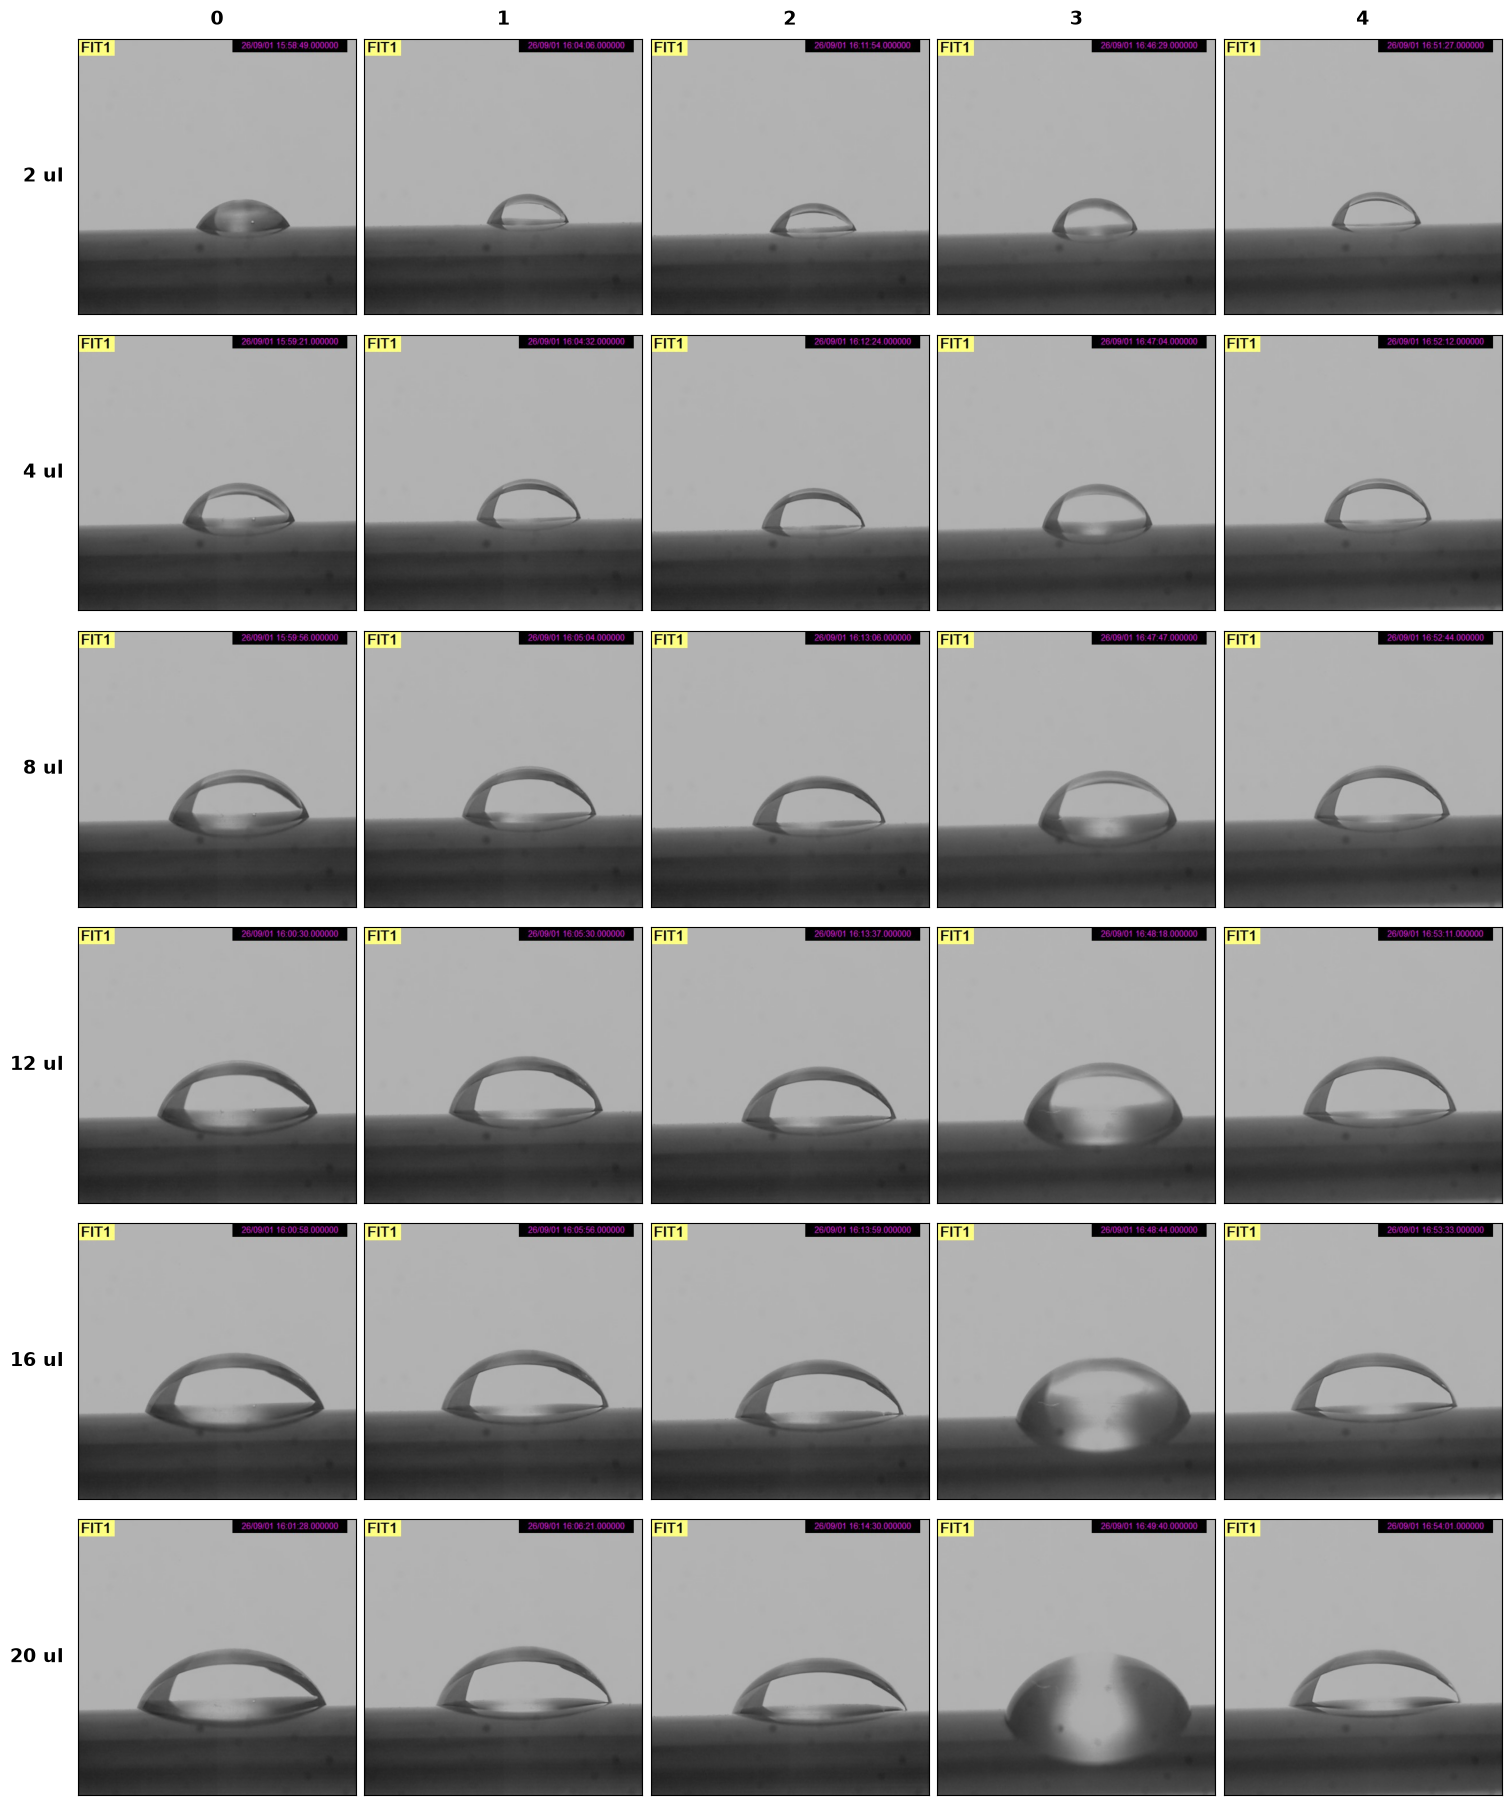
\includegraphics[width=\linewidth]{../Collages/collage_PMMA_2-30ul_10mm_side.png}
        \caption{Measurements on the \SI{10}{\milli\meter} PMMA cylinder from the side perspective.}
    \end{figure}

    \begin{figure}[H]
        \centering
        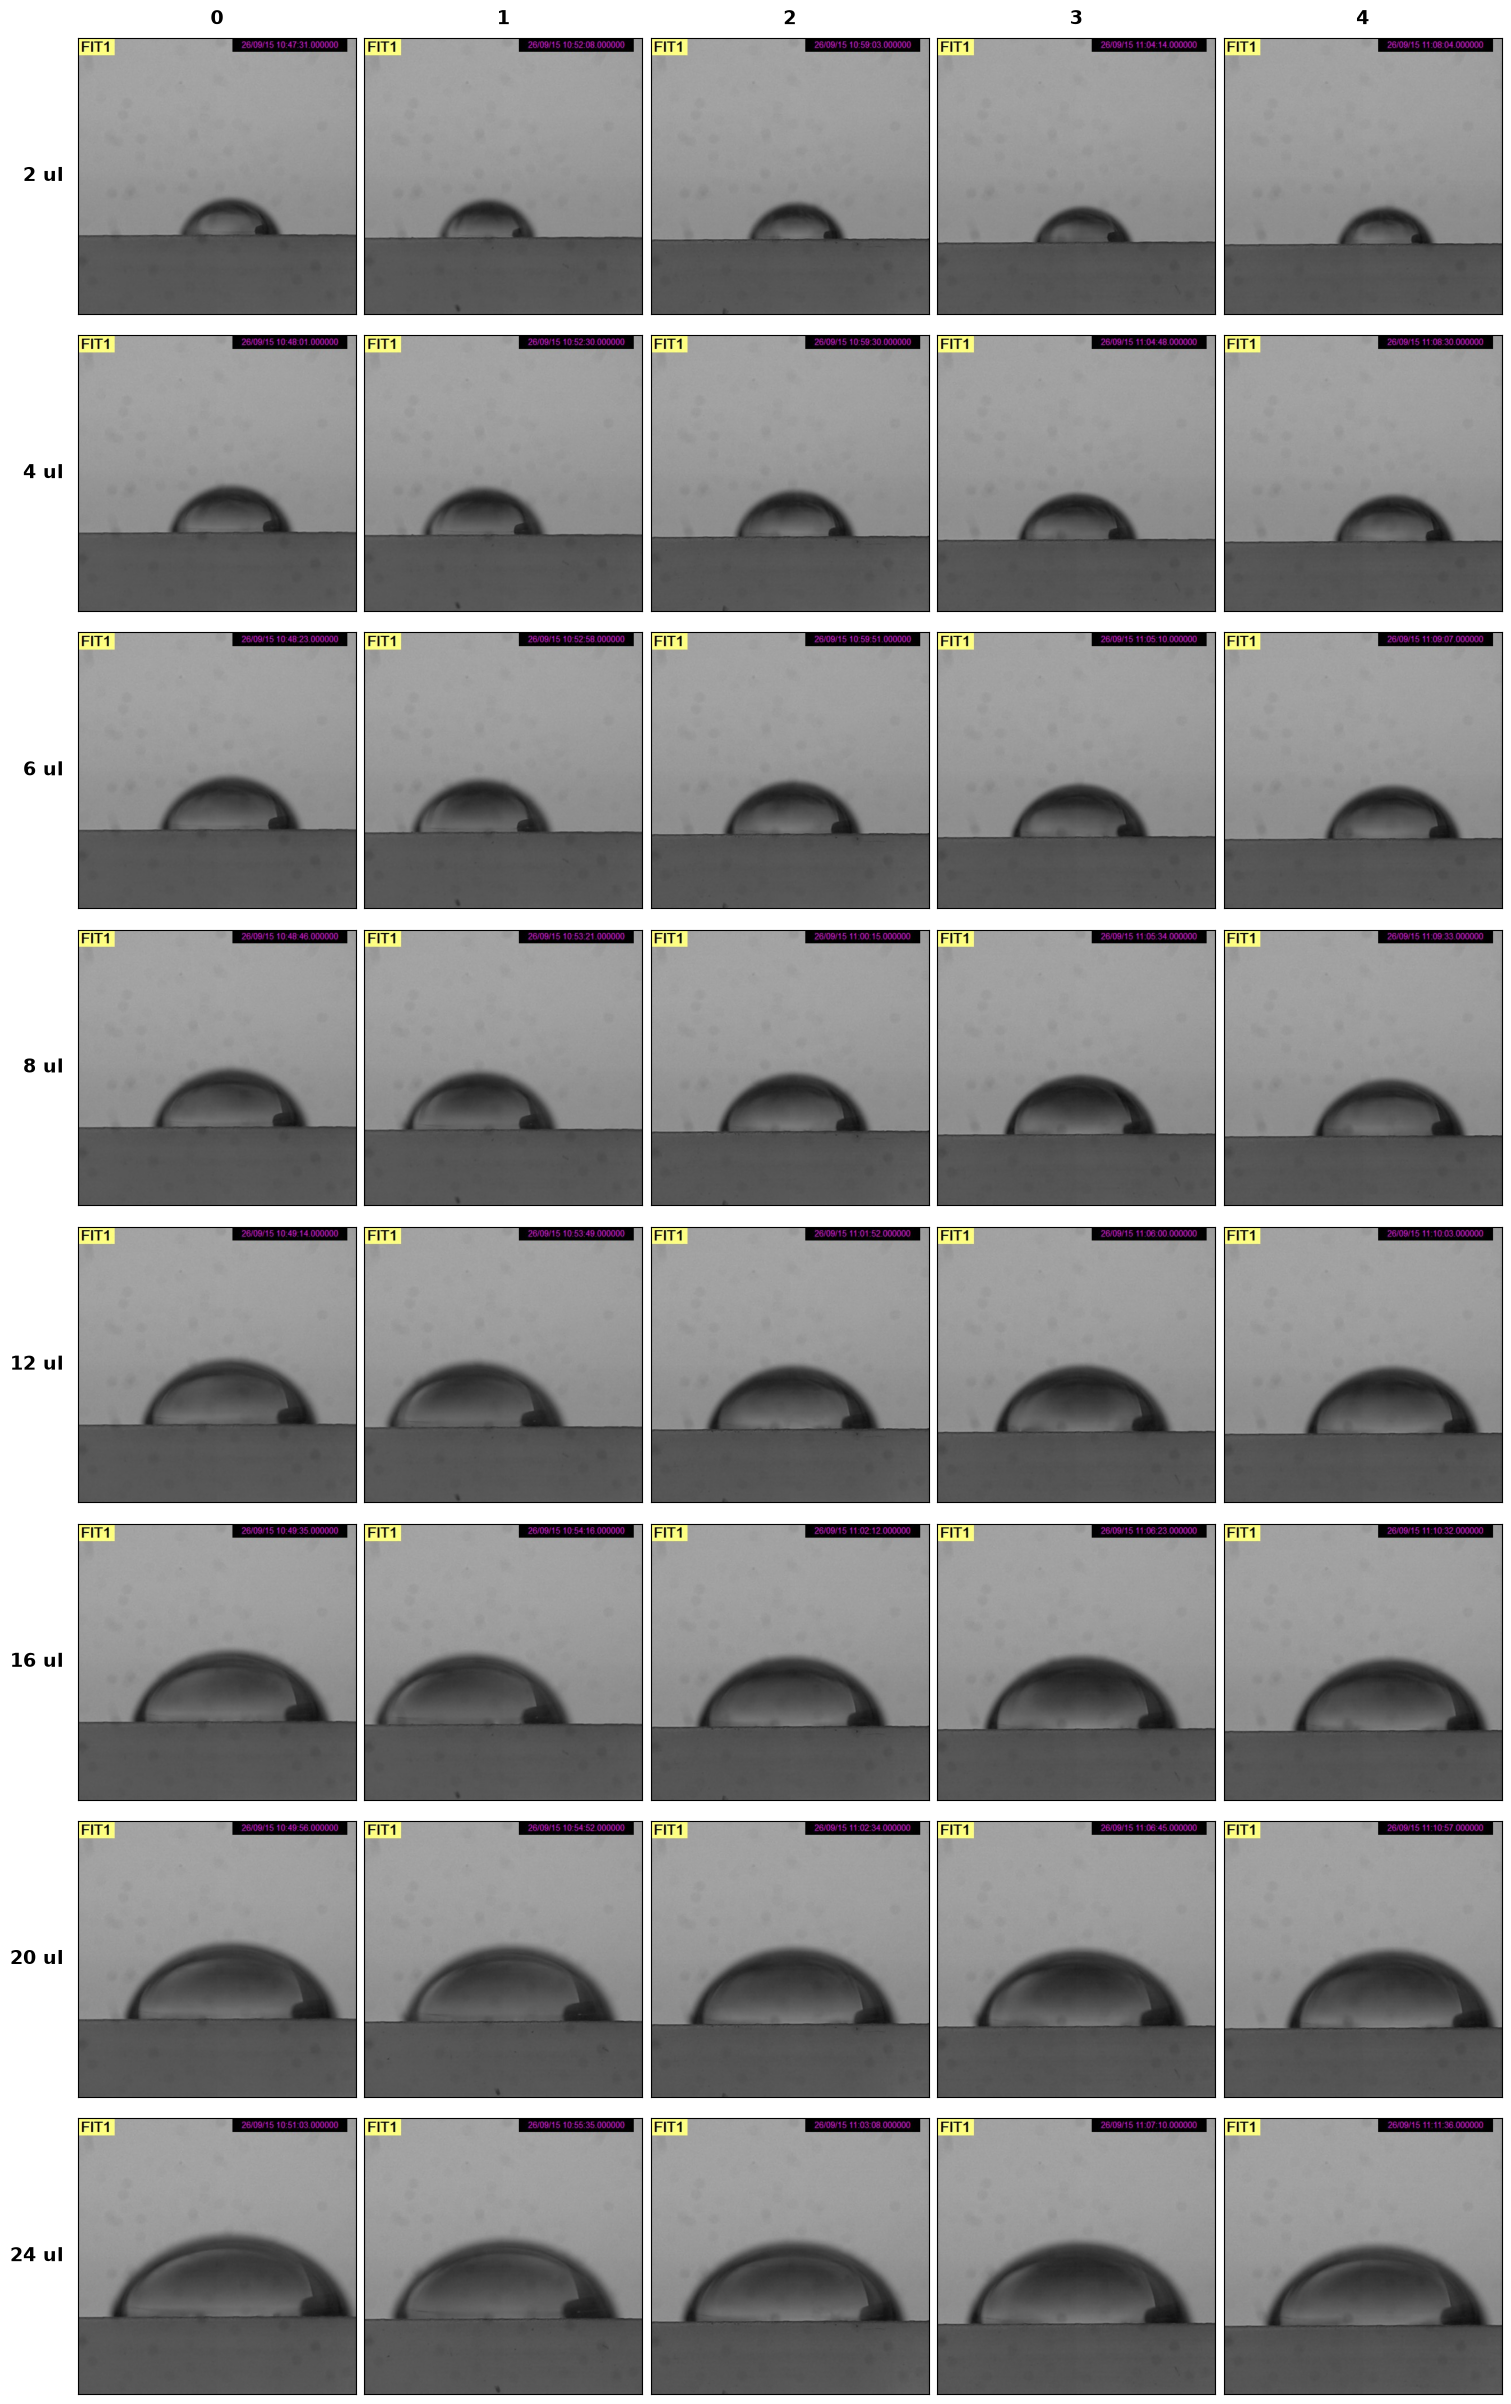
\includegraphics[width=0.85\linewidth]{../Collages/collage_PMMA_2-24ul_00mm_PMMA.png}
        \caption{Measurements on the flat PMMA substrate.}
    \end{figure}


\subsection{Measurement Collages on PET}
    \label{app:collages_PET}

    \begin{figure}[H]
        \centering
        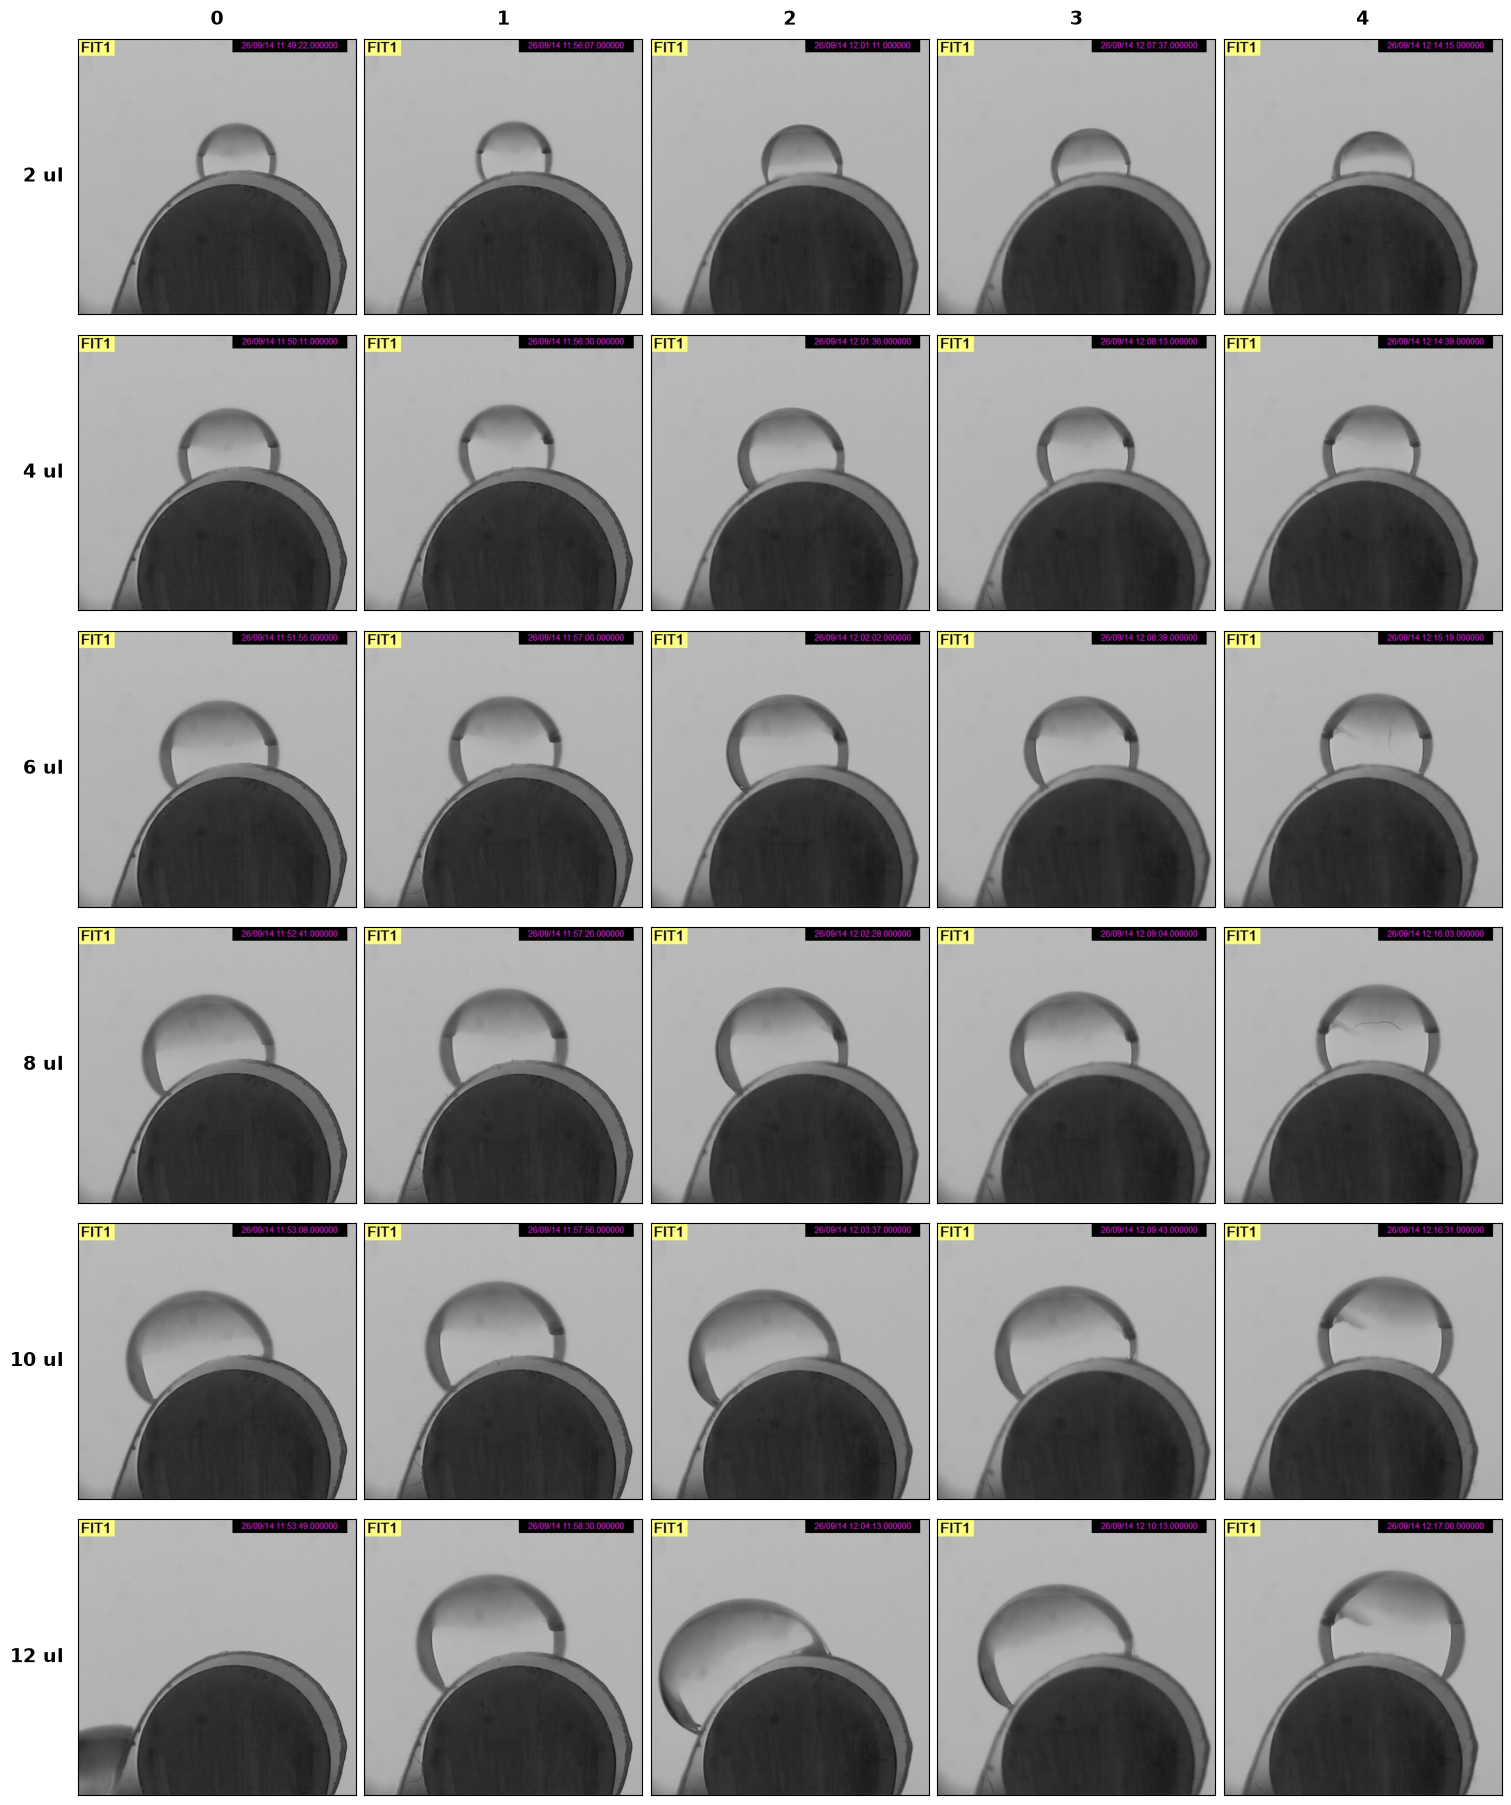
\includegraphics[width=\linewidth]{../Collages/collage_PET_2-12ul_04mm_front.png}
        \caption{Measurements on the \SI{4}{\milli\meter} PET cylinder from the front perspective.}
    \end{figure}

    \begin{figure}[H]
        \centering
        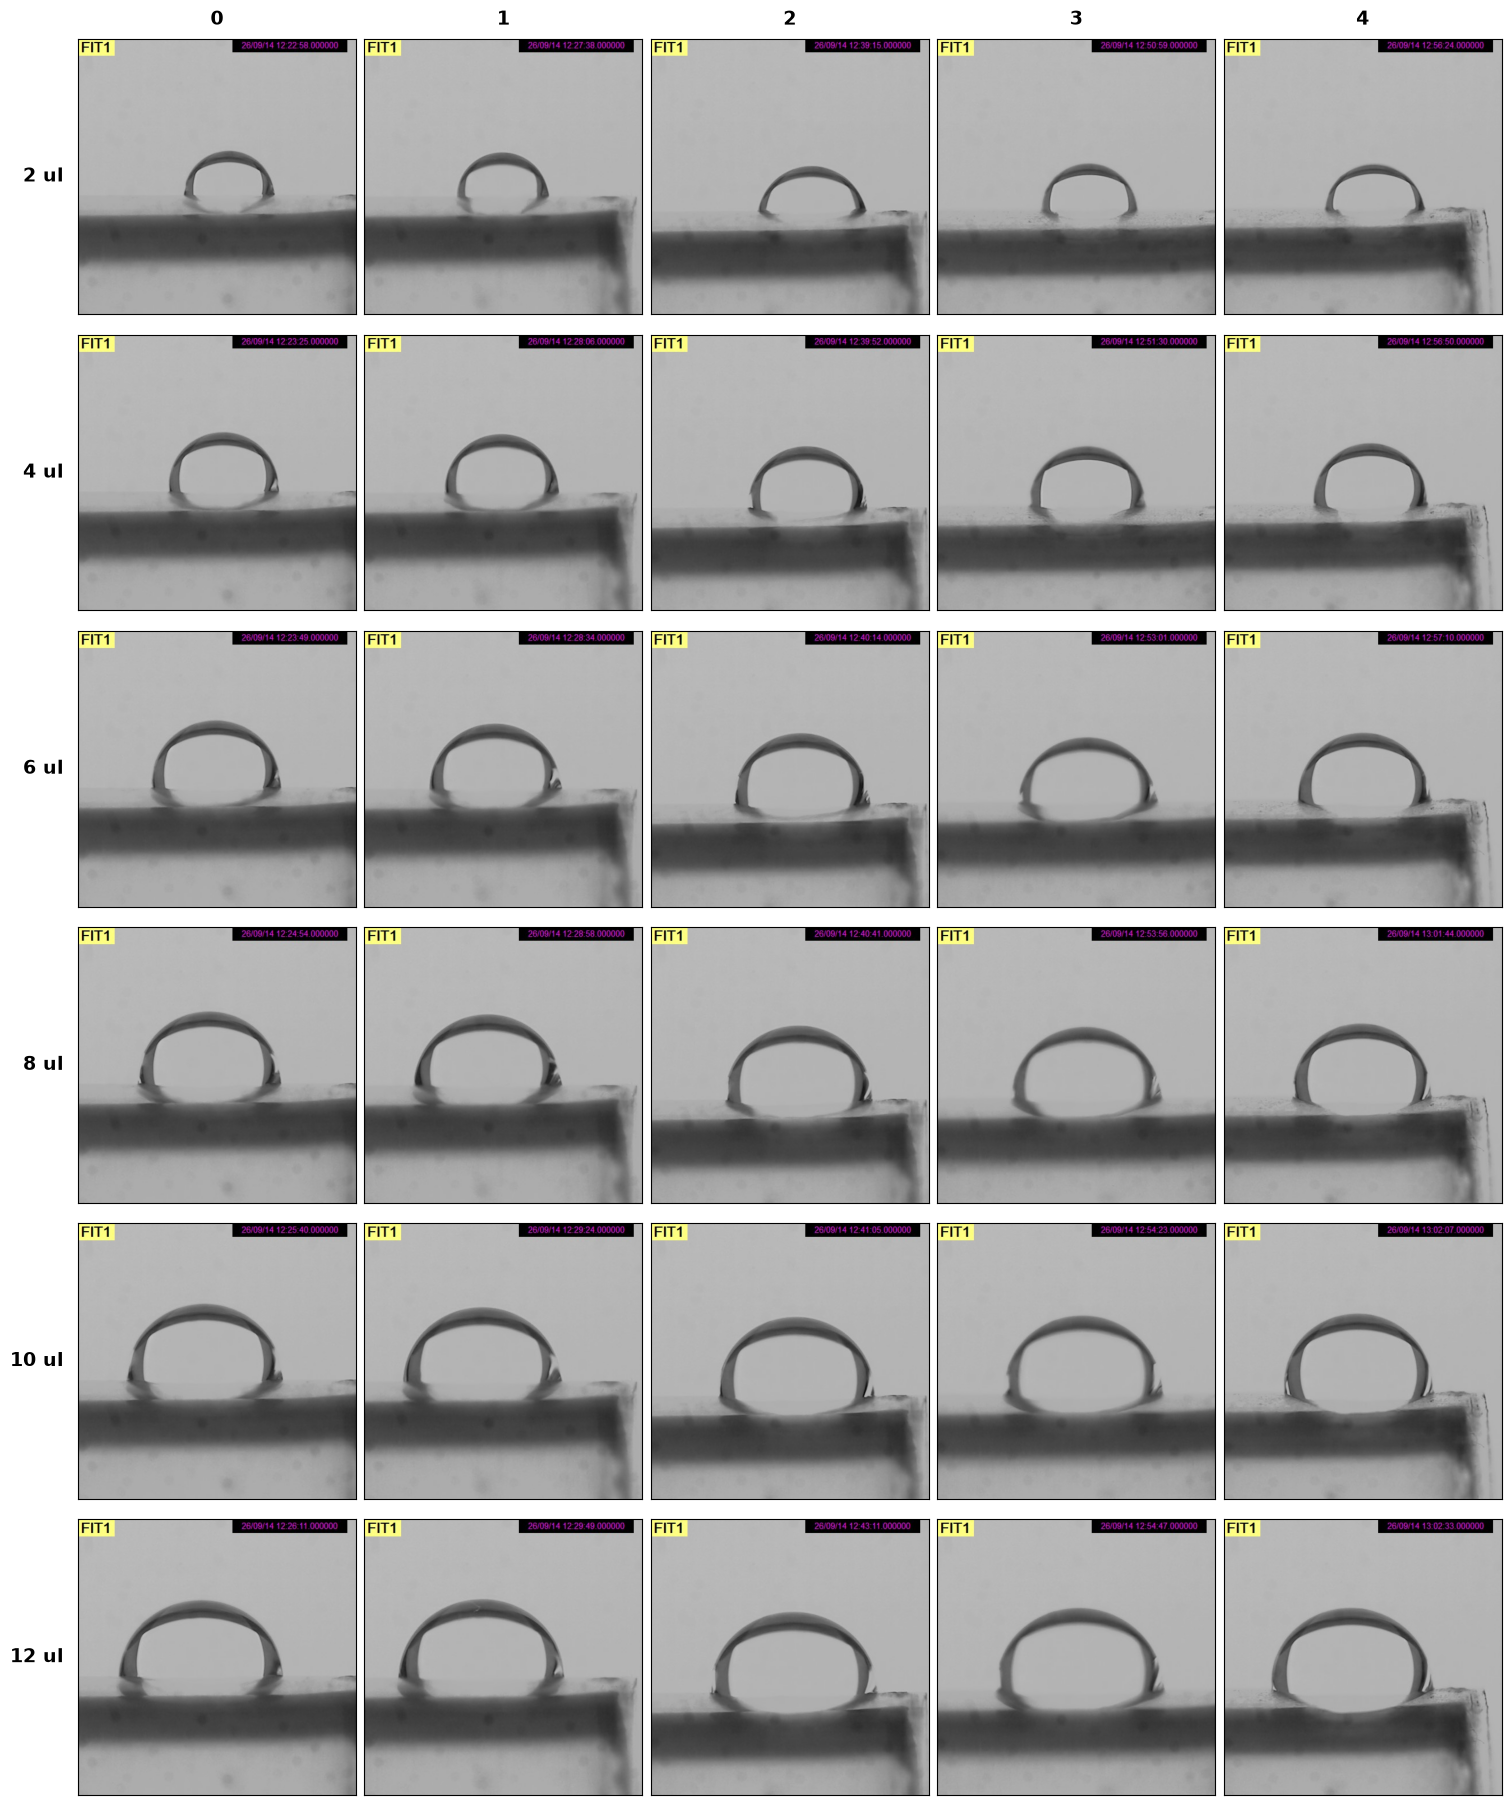
\includegraphics[width=\linewidth]{../Collages/collage_PET_2-12ul_04mm_side.png}
        \caption{Measurements on the \SI{4}{\milli\meter} PET cylinder from the side perspective.}
    \end{figure}

    \begin{figure}[H]
        \centering
        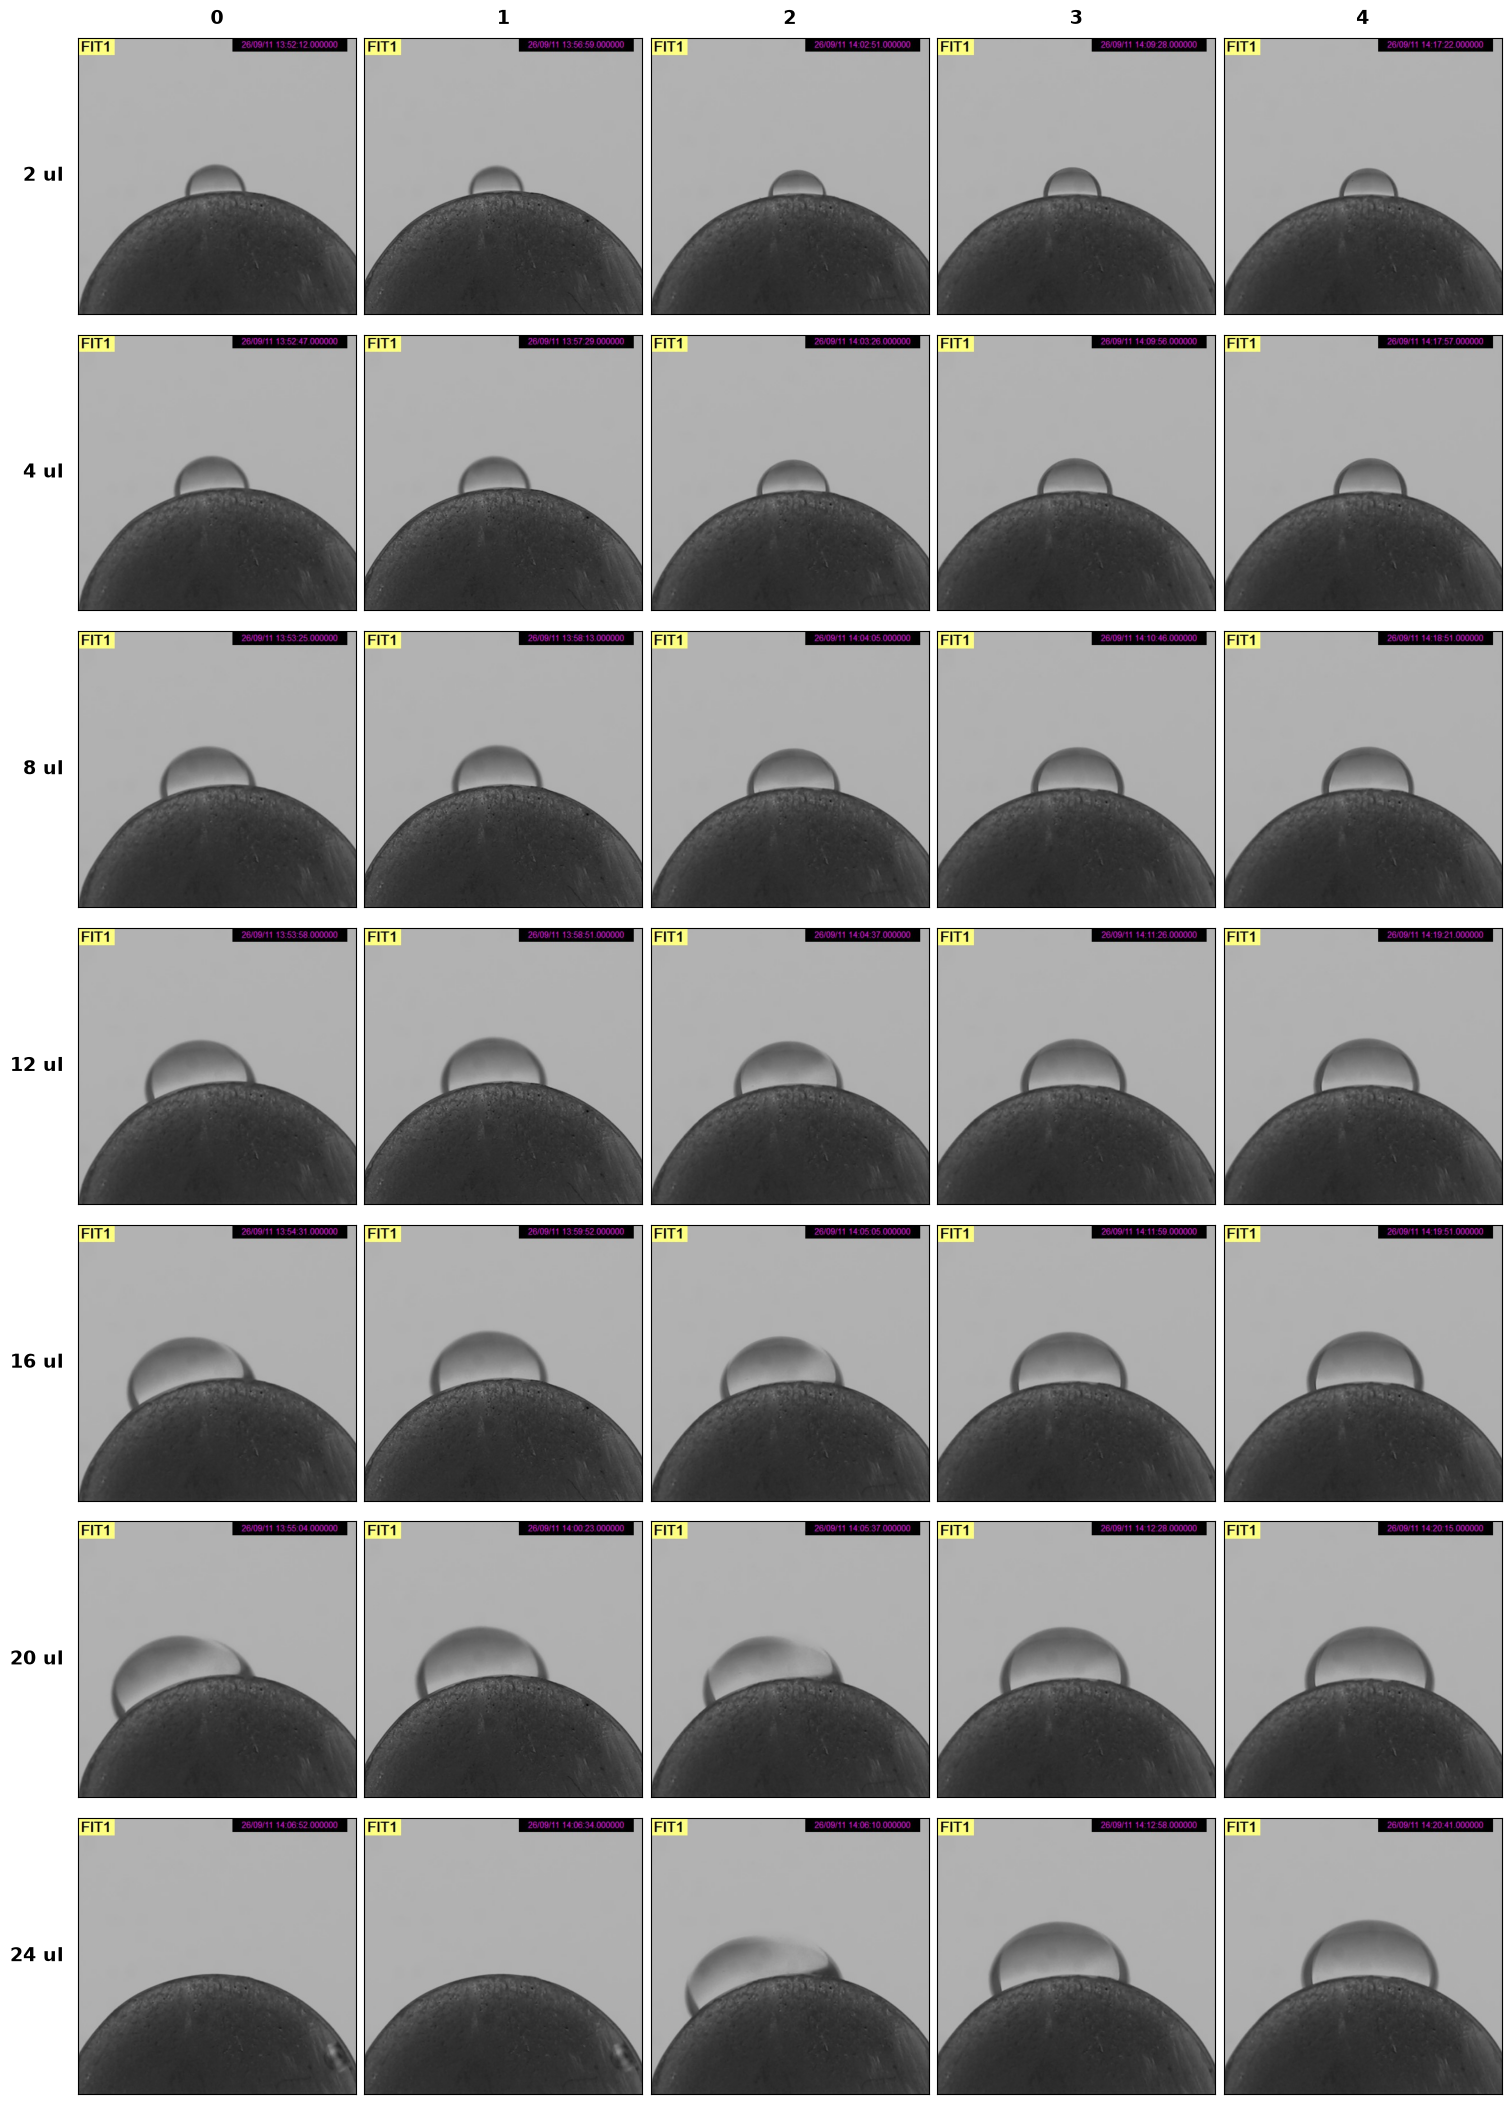
\includegraphics[width=0.95\linewidth]{../Collages/collage_PET_2-24ul_10mm_front.png}
        \caption{Measurements on the \SI{10}{\milli\meter} PET cylinder from the front perspective.}
    \end{figure}

    \begin{figure}[H]
        \centering
        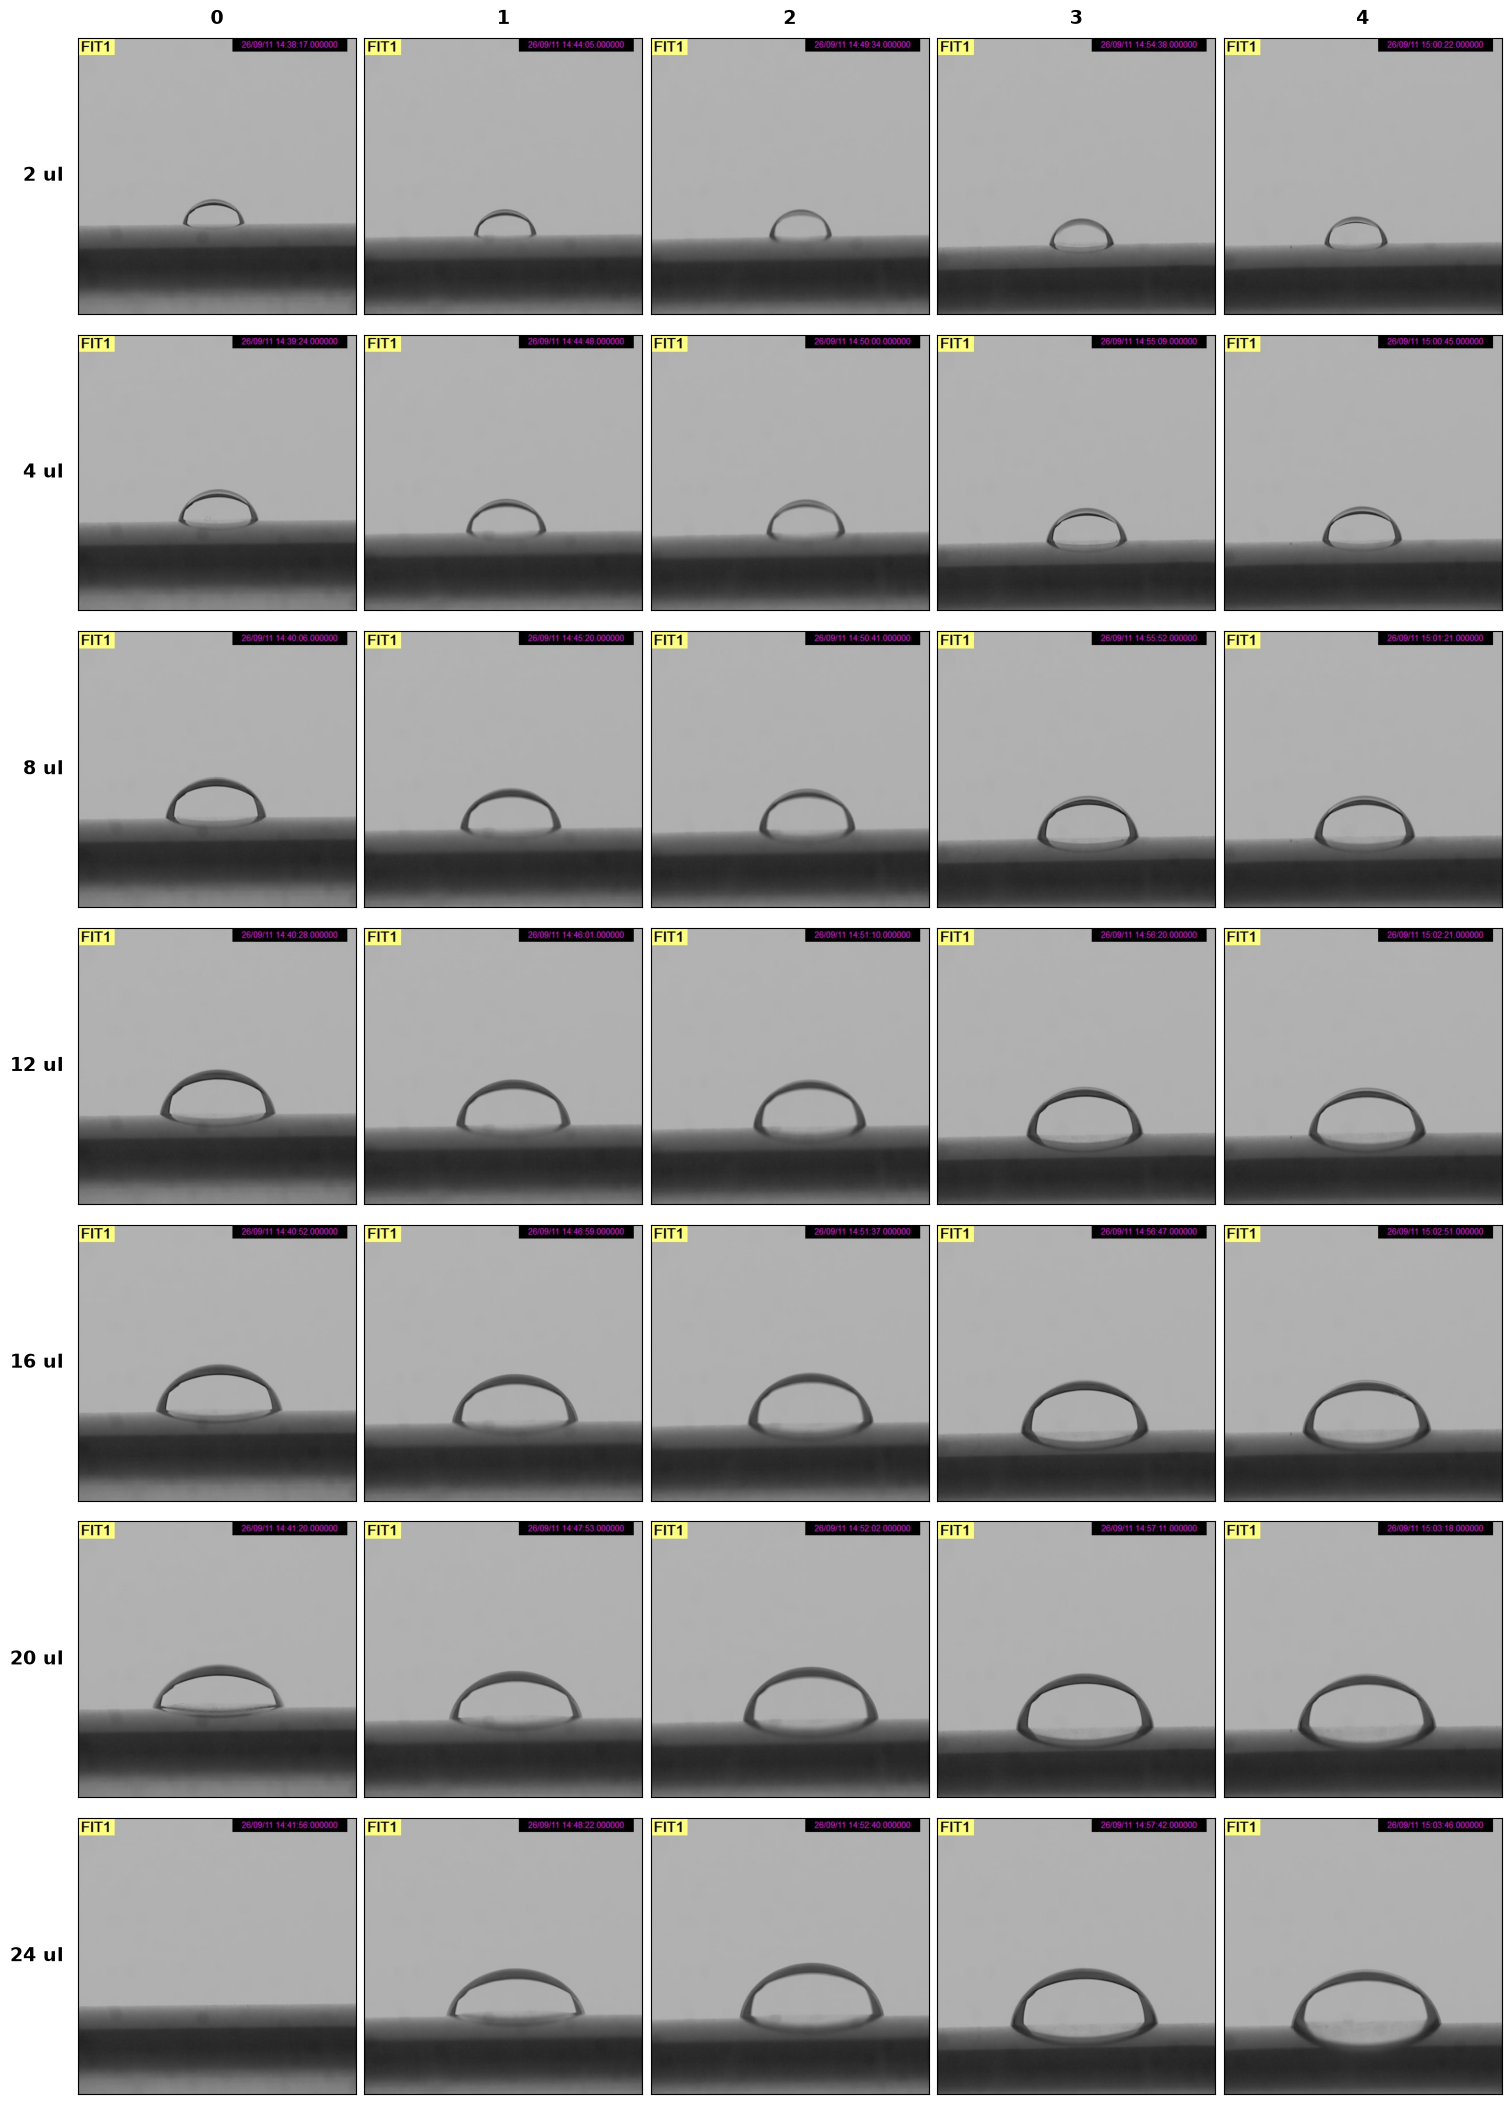
\includegraphics[width=0.95\linewidth]{../Collages/collage_PET_2-24ul_10mm_side.png}
        \caption{Measurements on the \SI{10}{\milli\meter} PET cylinder from the side perspective.}
    \end{figure}

    \begin{figure}[H]
        \centering
        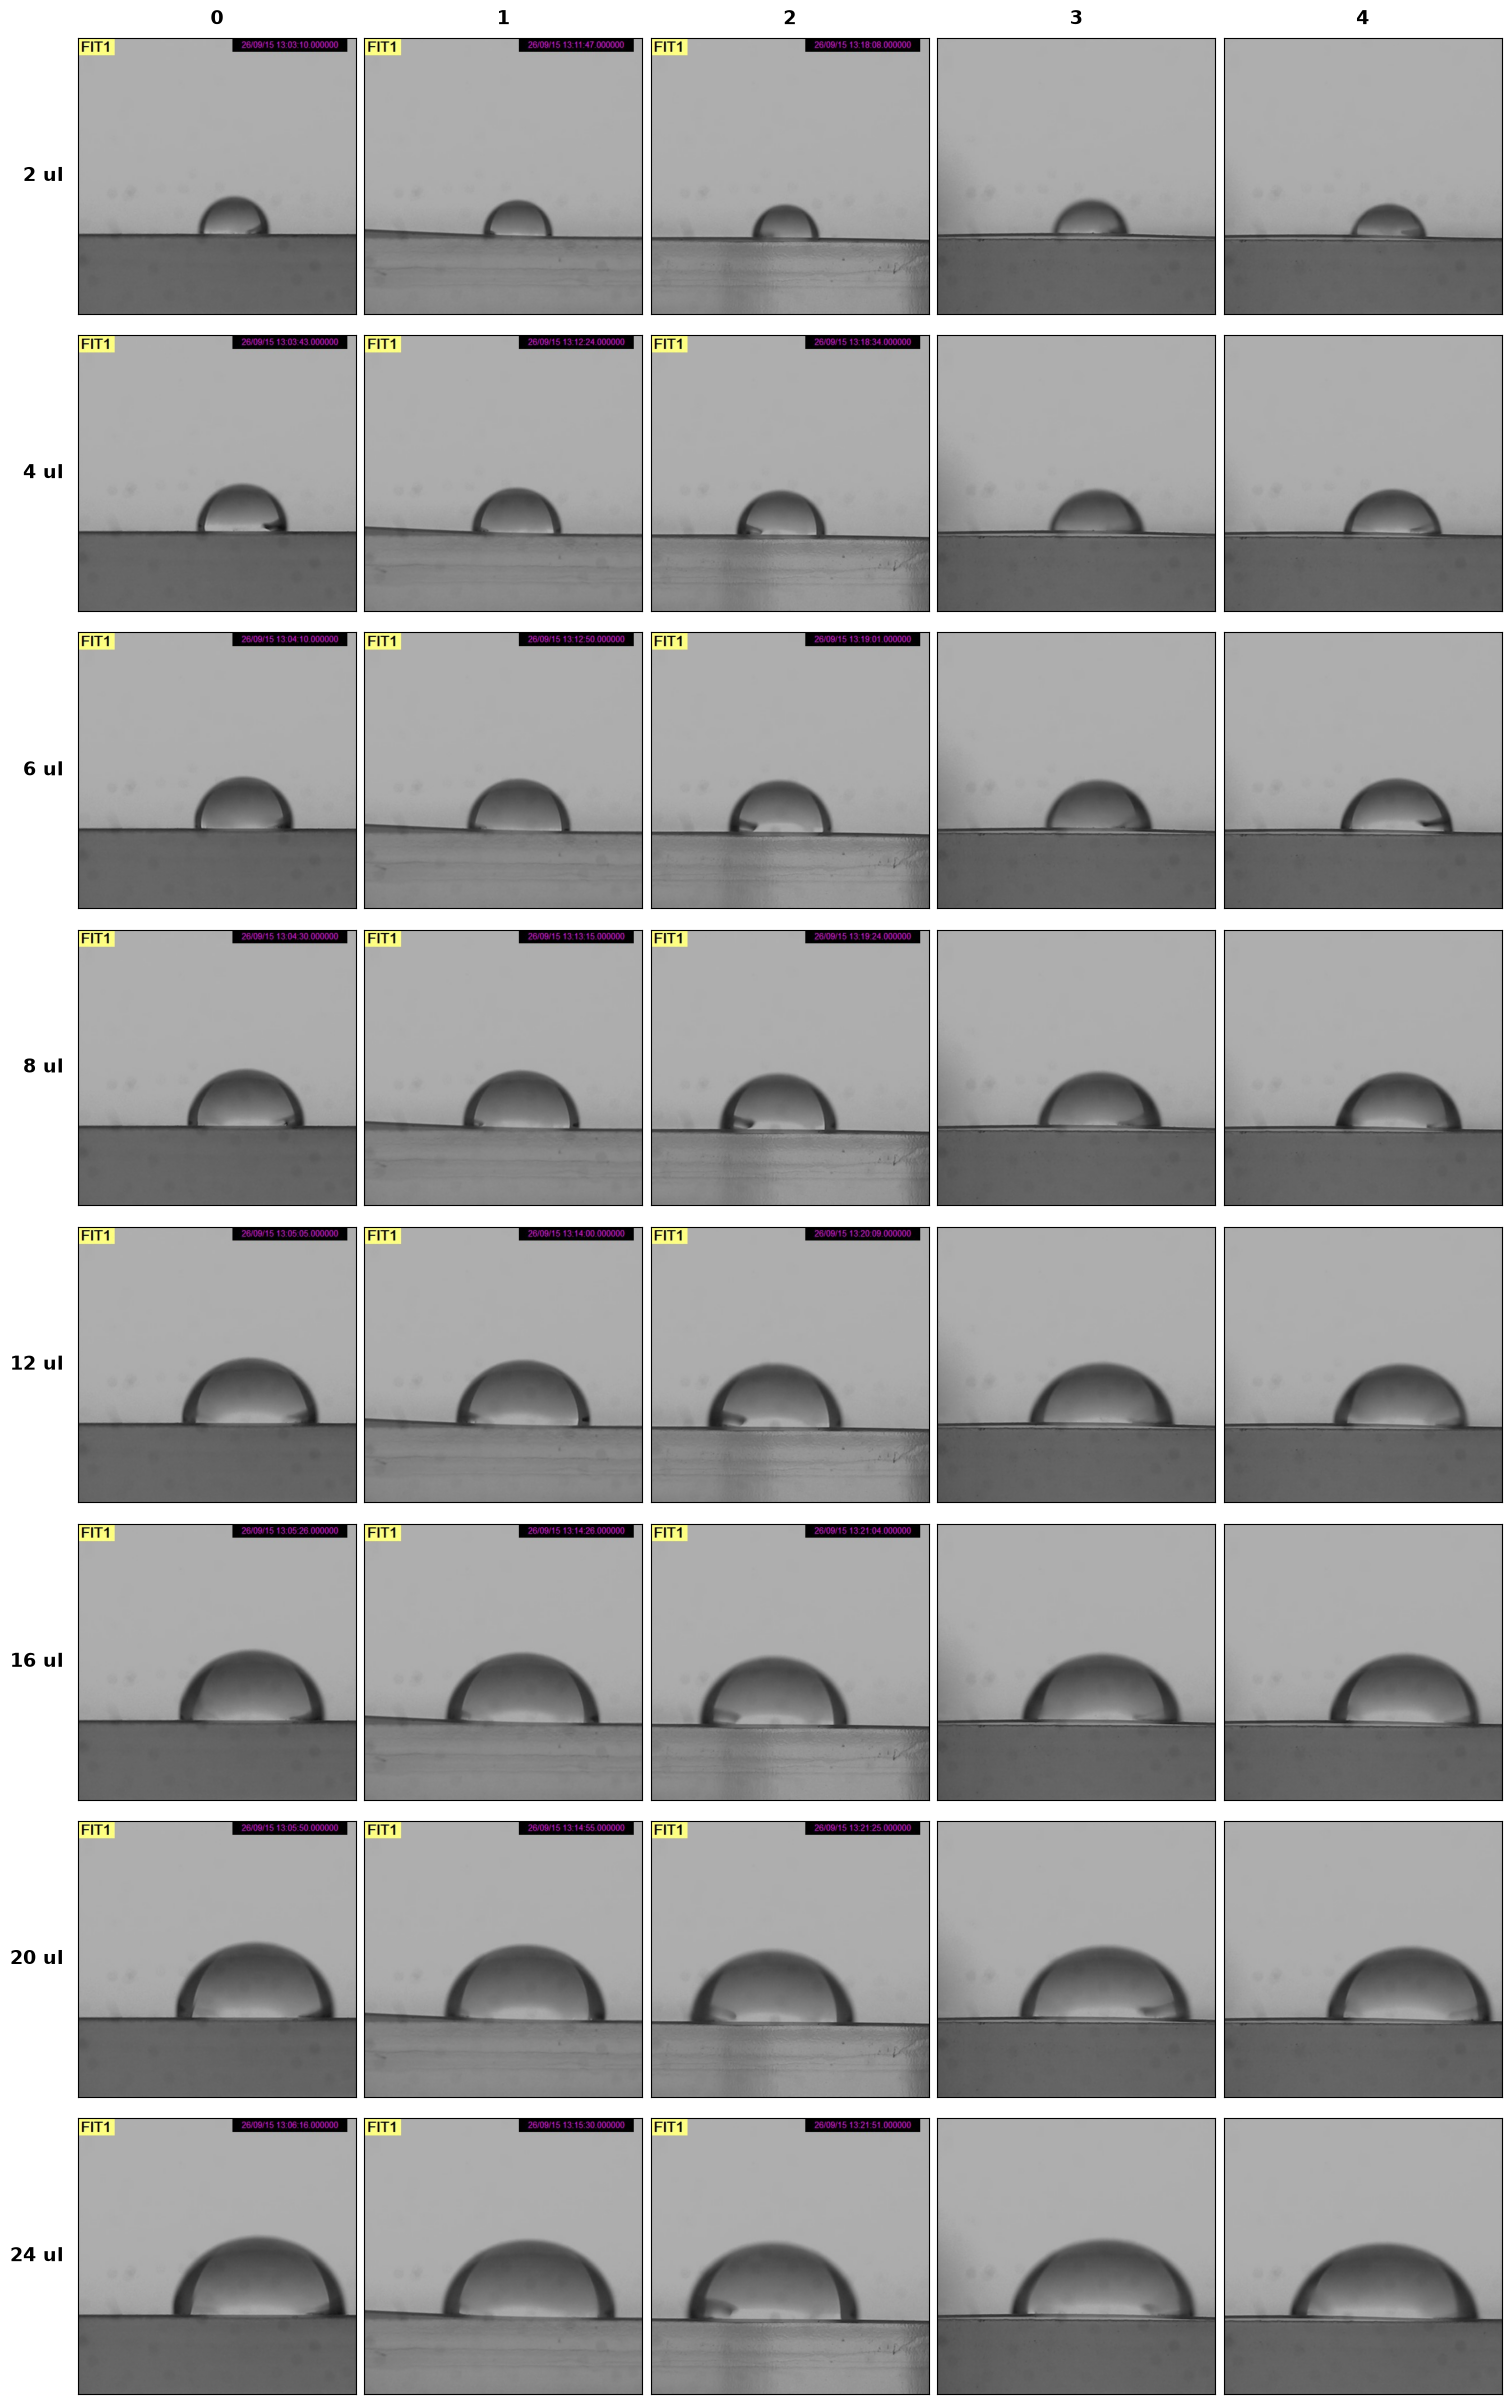
\includegraphics[width=0.85\linewidth]{../Collages/collage_PET_2-24ul_00mm_PET.png}
        \caption{Measurements on the flat PET substrate.}
    \end{figure}

